\documentclass[aspectratio=169,xcolor=dvipsnames,,table,compress]{beamer}
\usepackage{datetime}
\usepackage{tikz}
\usepackage{nicefrac}
\usepackage{multirow}
\usepackage{pgf}
\usetikzlibrary{arrows,automata,positioning}
\usepackage{amssymb,amsmath}
\usepackage{slashed}
\usepackage{bm}
\usepackage{graphicx}
\usepackage[percent]{overpic}
\usepackage{color}
% \usepackage{appendixnumberbeamer}
\usepackage{listings}
\usepackage{hyperref}
% \usepackage[table]{xcolor}% http://ctan.org/pkg/xcolor
\usepackage{hhline}
\usepackage{caption}
\usepackage[normalem]{ulem}
\usepackage[export]{adjustbox}
\usepackage{soul}
% \usepackage{subcaption}
\newcommand{\thus}{$\Rightarrow$~}
\newcommand{\ttbar}{\ensuremath{t\bar{t}}~}
\newcommand{\sgn}{\text{sign}}
\newcommand{\p}{\hat{p}}
\newcommand{\q}{\mathbf{q}}
\newcommand{\tv}{\tilde{\ve}}
\newcommand{\proj}{\text{\proj}}
\newcommand{\Z}{\mathbb{Z}}
\newcommand{\Q}{\mathbb{Q}}
\newcommand{\C}{\mathbb{C}}
\newcommand{\R}{\mathbb{R}}
\newcommand{\ov}{\overline}
\newcommand{\tr}{\text{Tr}}
\newcommand{\spane}{\text{span}}
\newcommand{\pp}[2]{\dfrac{\partial #1}{\partial #2}}
\newcommand{\dd}[2]{\dfrac{d #1}{d #2}}
\newcommand{\ddt}[2]{\dfrac{\partial^2 #1}{\partial #2^2}}
\newcommand{\dre}{\dot{\re}}
\newcommand{\met}{ E_\text{T}^\text{miss}}
\newcommand{\ptmiss}{ p_\text{T}^\text{miss}}
\newcommand{\pt}{ p_\text{T}}
\newcommand{\metphi}{\phi_{\slashed E_T}}
\newcommand{\qbar}{\bar{q}}
\newcommand{\bbar}{\bar{b}}
\newcommand{\metsig}{\slashed E_{T,\text{sig}}}
\newcommand{\bness}{b\text{ness}}
\newcommand{\F}{\mathbf{F}}
\newcommand{\E}{\mathbf{E}}
\newcommand{\out}{\mathbf{o}}
\newcommand{\inp}{\mathbf{i}}
\newcommand{\w}{\mathbf{w}}
\newcommand{\Xn}[1]{{x}^{(#1)}}
\newcommand{\yn}[1]{y^{(#1)}}
\newcommand{\z}{{z}}
\newcommand{\zn}[1]{z^{(#1)}}
\newcommand{\esig}{\epsilon_\text{sig}}
\newcommand{\ebg}{\epsilon_\text{bg}}
\newcommand{\gev}{\text{GeV}}
\newcommand{\tev}{\text{TeV}}
\newcommand{\gevp}{\text{GeV}/c}
\newcommand{\gevm}{\text{GeV}/c^2}
\newcommand{\tbar}{\bar{t}}
\newcommand{\D}{\mathcal{D}}
\newcommand{\mlink}[1]{\textcolor{maroon}{\bf {#1}}}
\newcommand{\mlinkmath}[1]{$\textcolor{maroon}{\bm {#1}}$}
\newcommand{\mlinksmall}[1]{#1}
\newcommand{\fns}{\footnotesize}
\newcommand{\msd}{m_\text{SD}}
\newcommand{\fb}{\text{fb}}
\newcommand{\mlc}[2][c]{%
  \begin{tabular}[#1]{@{}c@{}}#2\end{tabular}}
\newcommand{\secpage}[1]{\begin{frame}[t]
\frametitle{~}
\vspace{15mm}
\begin{center}
  \LARGE{#1}
\end{center}
\end{frame}
}
\newcommand{\X}{\mlink{X}}
\newcommand{\rc}{\cellcolor{maroon!75}}
\newcommand{\drc}{\cellcolor{maroon}}
\newcommand{\gc}{\cellcolor{mygrey}}
\newcommand{\N}{\mlink{N}}
\newcommand{\monojet}{mono-\mlink{jet}}
\newcommand{\ttdm}{$\textcolor{maroon}{\bm{\ttbar}}\mathrm{+DM}$}

\newcommand{\backupbegin}{
   \newcounter{finalframe}
   \setcounter{finalframe}{\value{framenumber}}
}
\newcommand{\backupend}{
   \setcounter{framenumber}{\value{finalframe}}
}
\newcommand{\bmu}{\textcolor{maroon}{\bm{\mu}}}
\newcommand{\bR}{\textcolor{maroon}{\bm{R}}}

\newdateformat{dmy}{\twodigit{\THEDAY}/\twodigit{\THEMONTH}/\THEYEAR}
\newdateformat{ymd}{\twodigit{\THEYEAR}/\twodigit{\THEMONTH}/\twodigit{\THEDAY}}

\usefonttheme{serif}


\DeclareMathOperator{\diag}{\text{diag}}
\DeclareMathOperator{\NN}{\text{NN}}
\DeclareMathOperator{\NLL}{\text{NLL}}
\usetheme{default}
\setbeamertemplate{navigation symbols}{}
\useoutertheme{infolines}

\addtobeamertemplate{frametitle}{}{%
  \begin{tikzpicture}[remember picture,overlay]
    \node[anchor=north east,yshift=0pt] at (current page.north east) {
      
\includegraphics[width=0.05\textwidth]{../figures/common/CMS_logo_bw.pdf}\hspace{.1mm}
      
\includegraphics[width=0.095\textwidth]{../figures/common/MIT-logo-black-red.pdf}
    };
  \end{tikzpicture}
}
\definecolor{maroon}{rgb}{0.64, 0.12, 0.20}
\definecolor{mygrey}{rgb}{0.4, 0.4, 0.4}
\usecolortheme{dove}
\setbeamercolor{enumerate item}{fg=black,bg=white}
\setbeamercolor{enumerate subitem}{fg=black,bg=white}
\setbeamercolor{itemize subitem}{fg=black,bg=white}
\setbeamercolor{itemize item}{fg=black,bg=white}
\setbeamercolor{item projected}{fg=white,bg=TAMIU}
\useoutertheme{infolines}
\setbeamertemplate{headline}{}
\useinnertheme{default}
\lstset{%
  language=C++,
%  backgroundcolor=\color{mygrey!25},
  basicstyle=\ttfamily,
  breaklines=true,
  columns=fullflexible
}

\newcommand{\mycite}[1]{{\tiny[#1]}}

\newcommand{\references}{
 \begin{frame}[t] \frametitle{References}
   \fns{
     [1] \url{https://en.wikipedia.org/wiki/Galaxy_rotation_curve}

     [2] \url{arXiv:astro-ph/9909252}

     [3] \url{hubblesite.org/image/1276/news\_release/2003-01}

     [4] \url{chandra.harvard.edu/photo/2006/1e0657/more.html}

     [5] 	\url{arXiv:astro-ph/1202.0090}

     [6] \url{https://kipac.stanford.edu/highlights/let-there-be-light-upon-dark-digging-deeper-dark-matter-lux}

     [7] \url{https://fermi.gsfc.nasa.gov/science/eteu/dm/}

     [8] \url{https://cms-docdb.cern.ch/cgi-bin/PublicDocDB/ShowDocument?docid=4172}

     [6] \url{physik.uzh.ch/en/researcharea/lhcb/outreach/StandardModel.html}

     [7] \url{arXiv:hep-ph/0802.1189}

     [8] \url{arXiv:hep-ph/1609.07473}
  }
 \end{frame}
}


\title[Ph.D. Thesis Defense]{Searching for Dark Matter Using Jets and Jet Substructure at the Large Hadron Collider}
\author[S. Narayanan]{
                      {
                       \href{mailto:sidn@mit.edu}{{Siddharth\,Narayanan}}
                       }
}
\date[\ymd\today]{Ph.D. Thesis Defense - \ymd\today}
\institute[MIT]{
                
\includegraphics[width=0.097\textwidth]{../figures/common/CMS_logo_bw.pdf}~
                
\includegraphics[width=0.185\textwidth]{../figures/common/MIT-logo-black-red.pdf}
                }

\begin{document}
{
  \usebackgroundtemplate{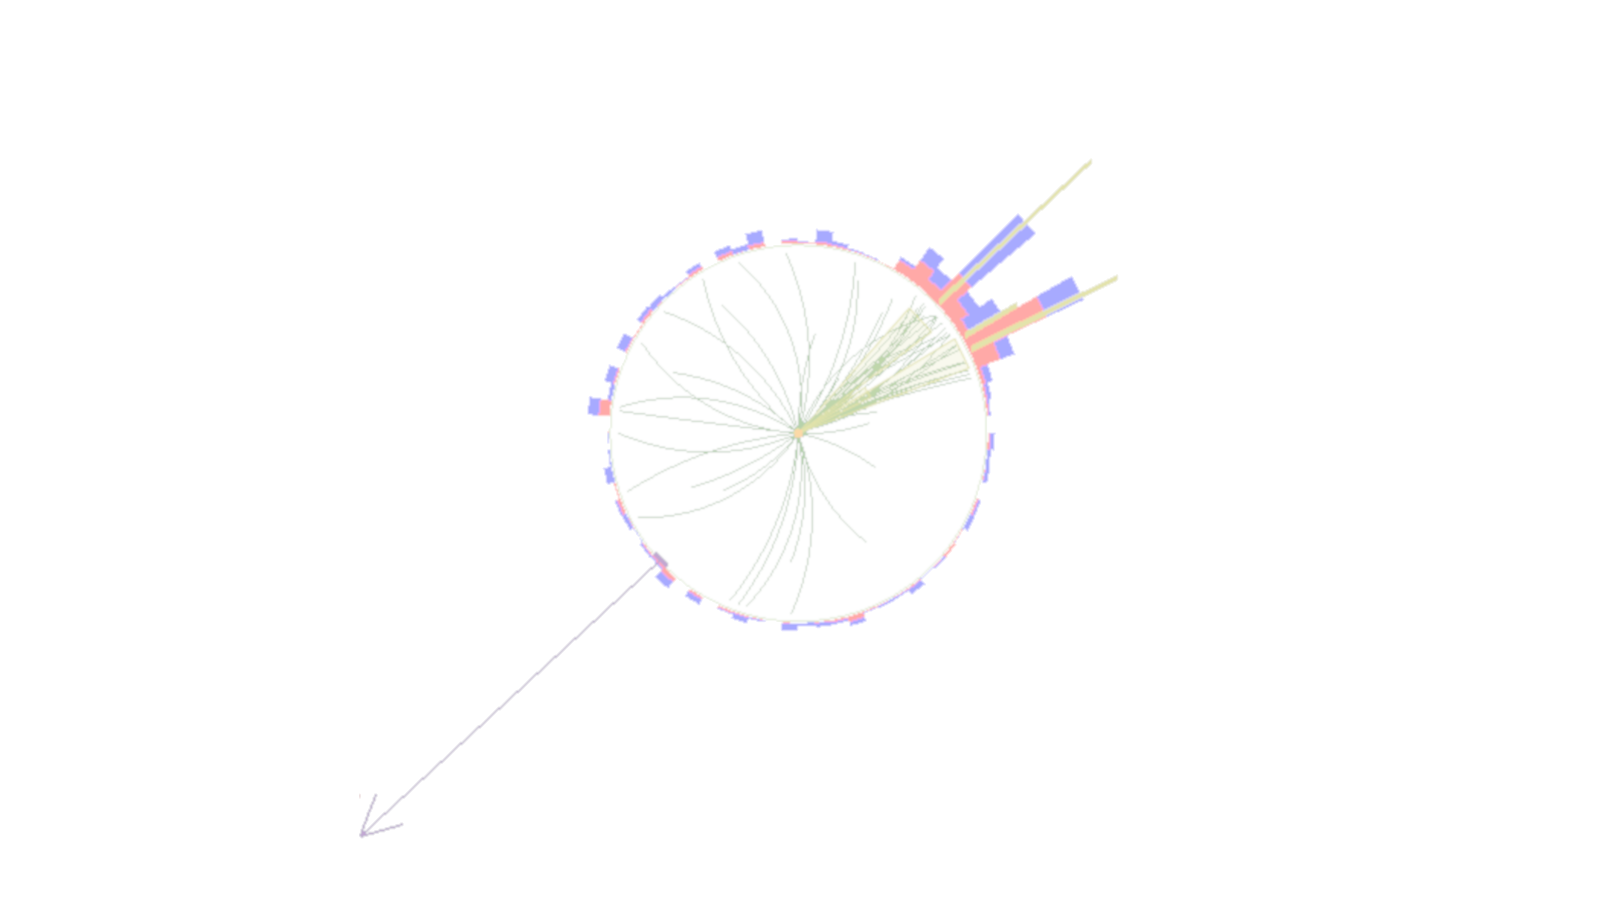
\includegraphics[height=\paperheight]{../figures/talk/1275337_634520340_334_RhoPhi3.png}}
  \begin{frame}
  \titlepage
  \end{frame}
}

\begin{frame}  \frametitle{Dark matter - in space}
  \vspace{-7mm}
  \begin{columns}[T]
    \begin{column}{0.5\textwidth}
      \begin{center}  
        { Strong astrophysical evidence for DM:} \\ 
        \vspace{3mm}
        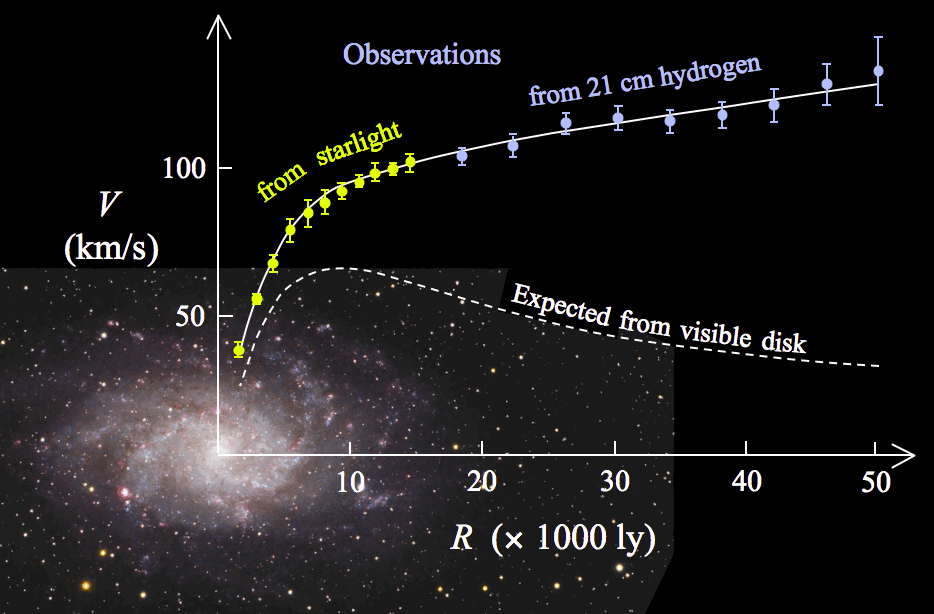
\includegraphics[width=0.7\textwidth]{../figures/talk/rotation.png} \mycite{1,2}
        \begin{columns}[T]
          \begin{column}{0.33\textwidth}
            \centering
            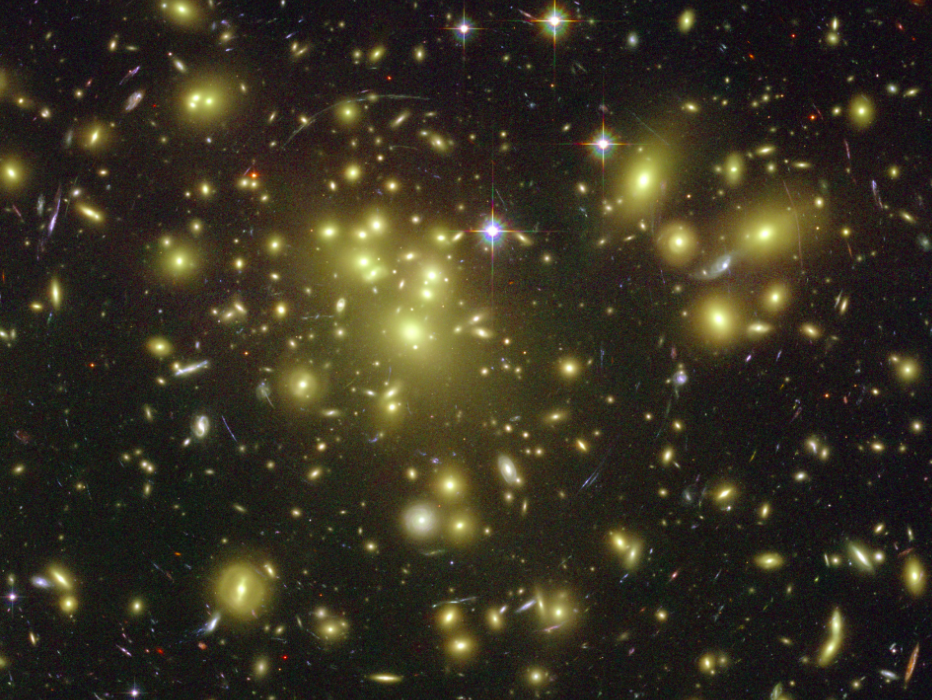
\includegraphics[width=\textwidth]{../figures/talk/lensing.png} \mycite{3}
          \end{column}
          \begin{column}{0.33\textwidth}
            \centering
            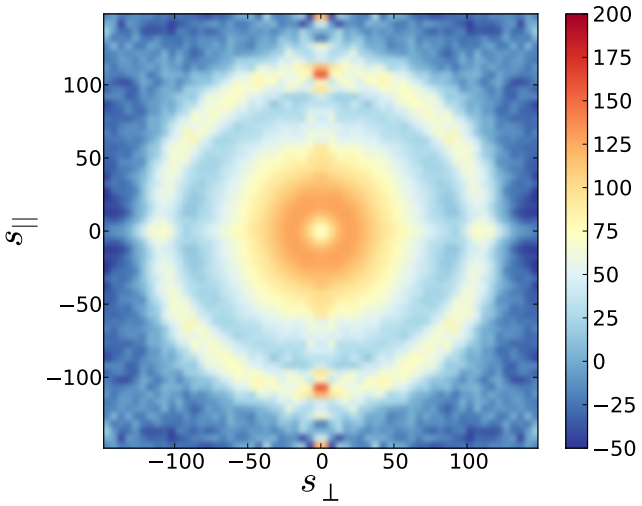
\includegraphics[width=\textwidth]{../figures/talk/cmb.png} \mycite{4}
          \end{column}
          \begin{column}{0.33\textwidth}
            \centering
            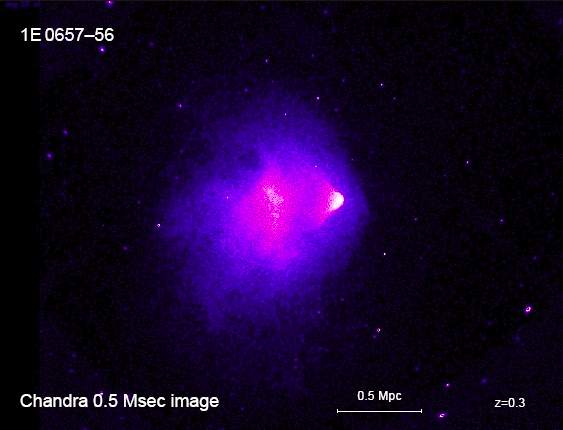
\includegraphics[width=\textwidth]{../figures/talk/bullet.png} \mycite{5}
          \end{column}
        \end{columns}
      \end{center}
      \pause 
    \end{column}
    \begin{column}{0.5\textwidth}
      \begin{center}
        {Weakly Interacting Massive Particles}
      \end{center}
      \begin{itemize}
        \item Weakly: DM-SM coupling $g_\chi \sim g$ 
        \item Massive: mass $m_\chi \sim 100$ GeV
        \item The ``WIMP miracle'':
          \[\Omega \propto  \frac{\rho}{\rho_{c}} \propto \frac{1}{\langle \sigma v \rangle} \]
          \[\Omega_\mathrm{meas.} = 0.12, \quad \Omega_\chi \sim 0.1\]
        \item Almost any DM model probed by a collider has a WIMP 
        \item Many other models exist (axions, MACHOs, \dots)
      \end{itemize}
    \end{column}
  \end{columns}
\end{frame}

\begin{frame} \frametitle{Dark matter - in a laboratory}
  \vspace{-7mm}
  \begin{columns}[T]
    \begin{column}{0.5\textwidth}
      \begin{center}  
        \only<1>{ 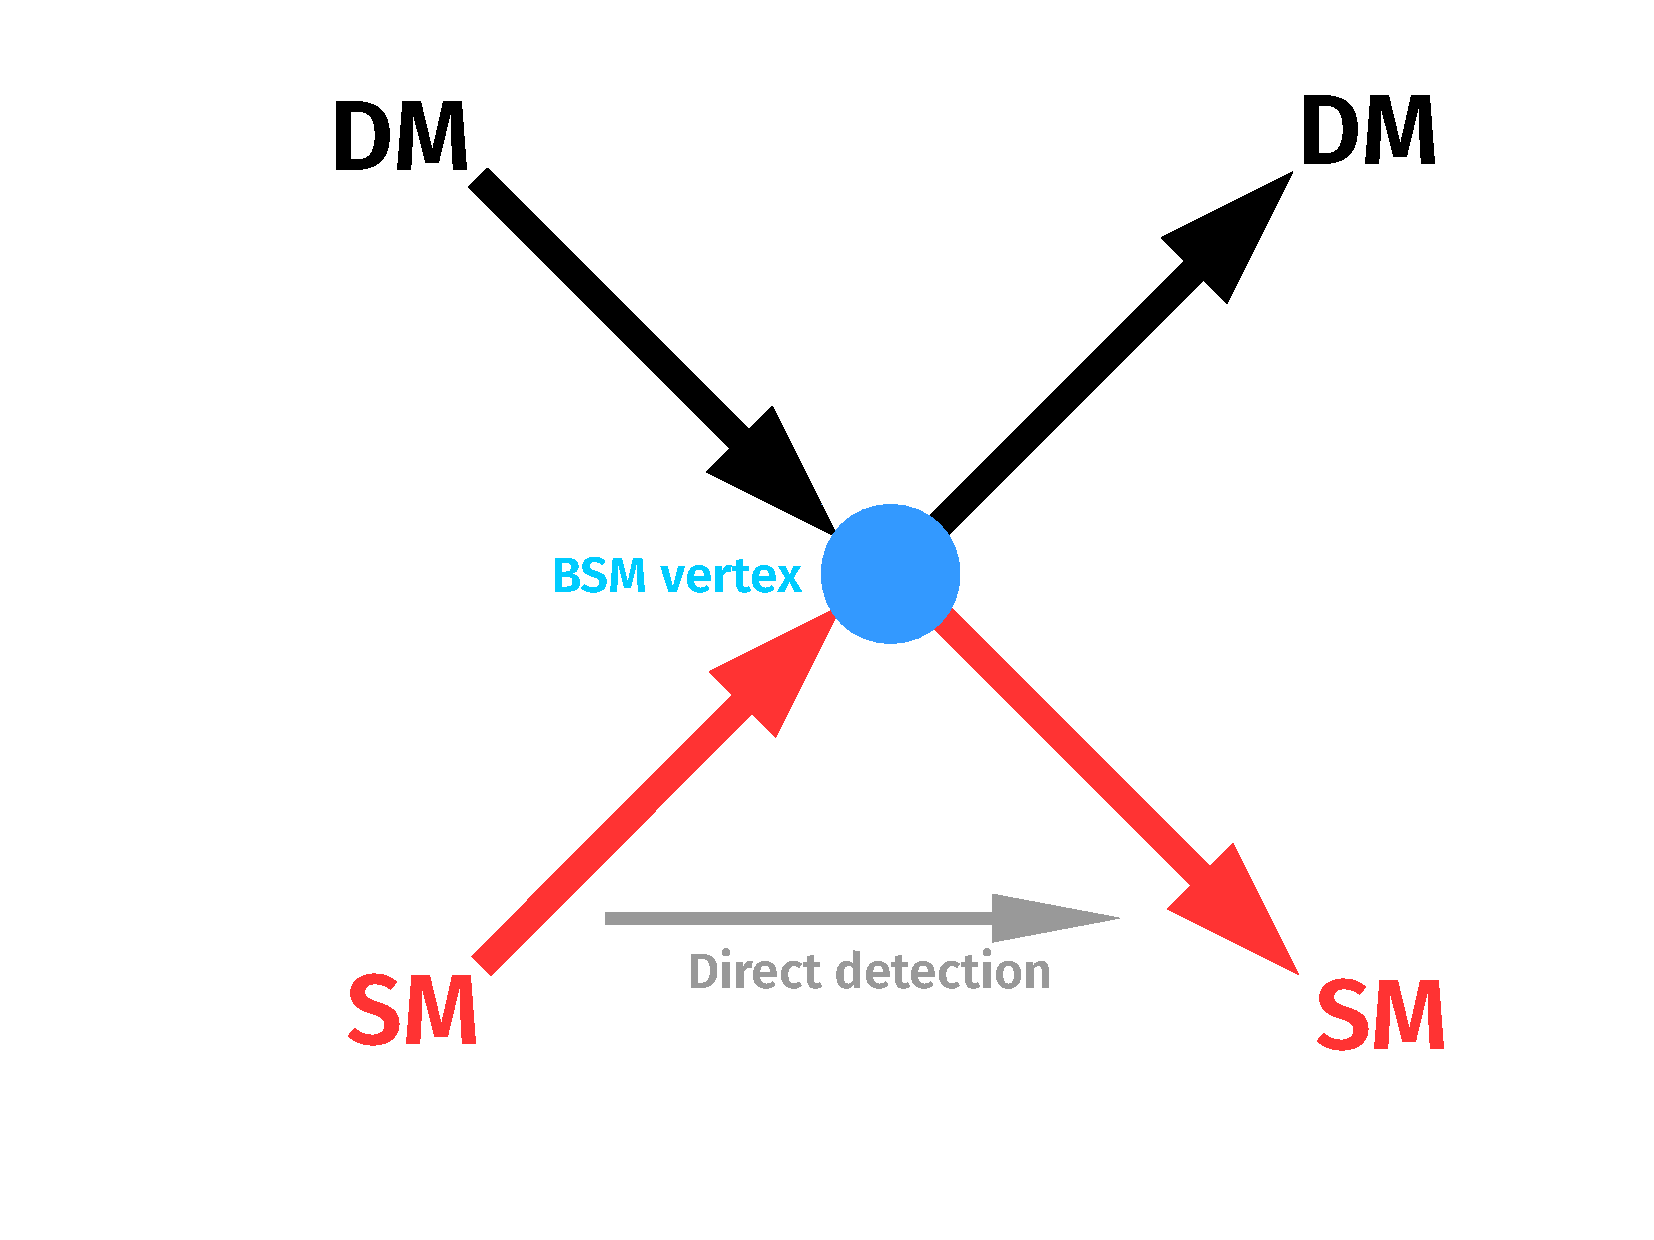
\includegraphics[width=\textwidth]{../figures/talk/dd.pdf} \\ 
                  Search for DM-SM interactions as Earth moves through DM halo
                 }
        \only<2>{ 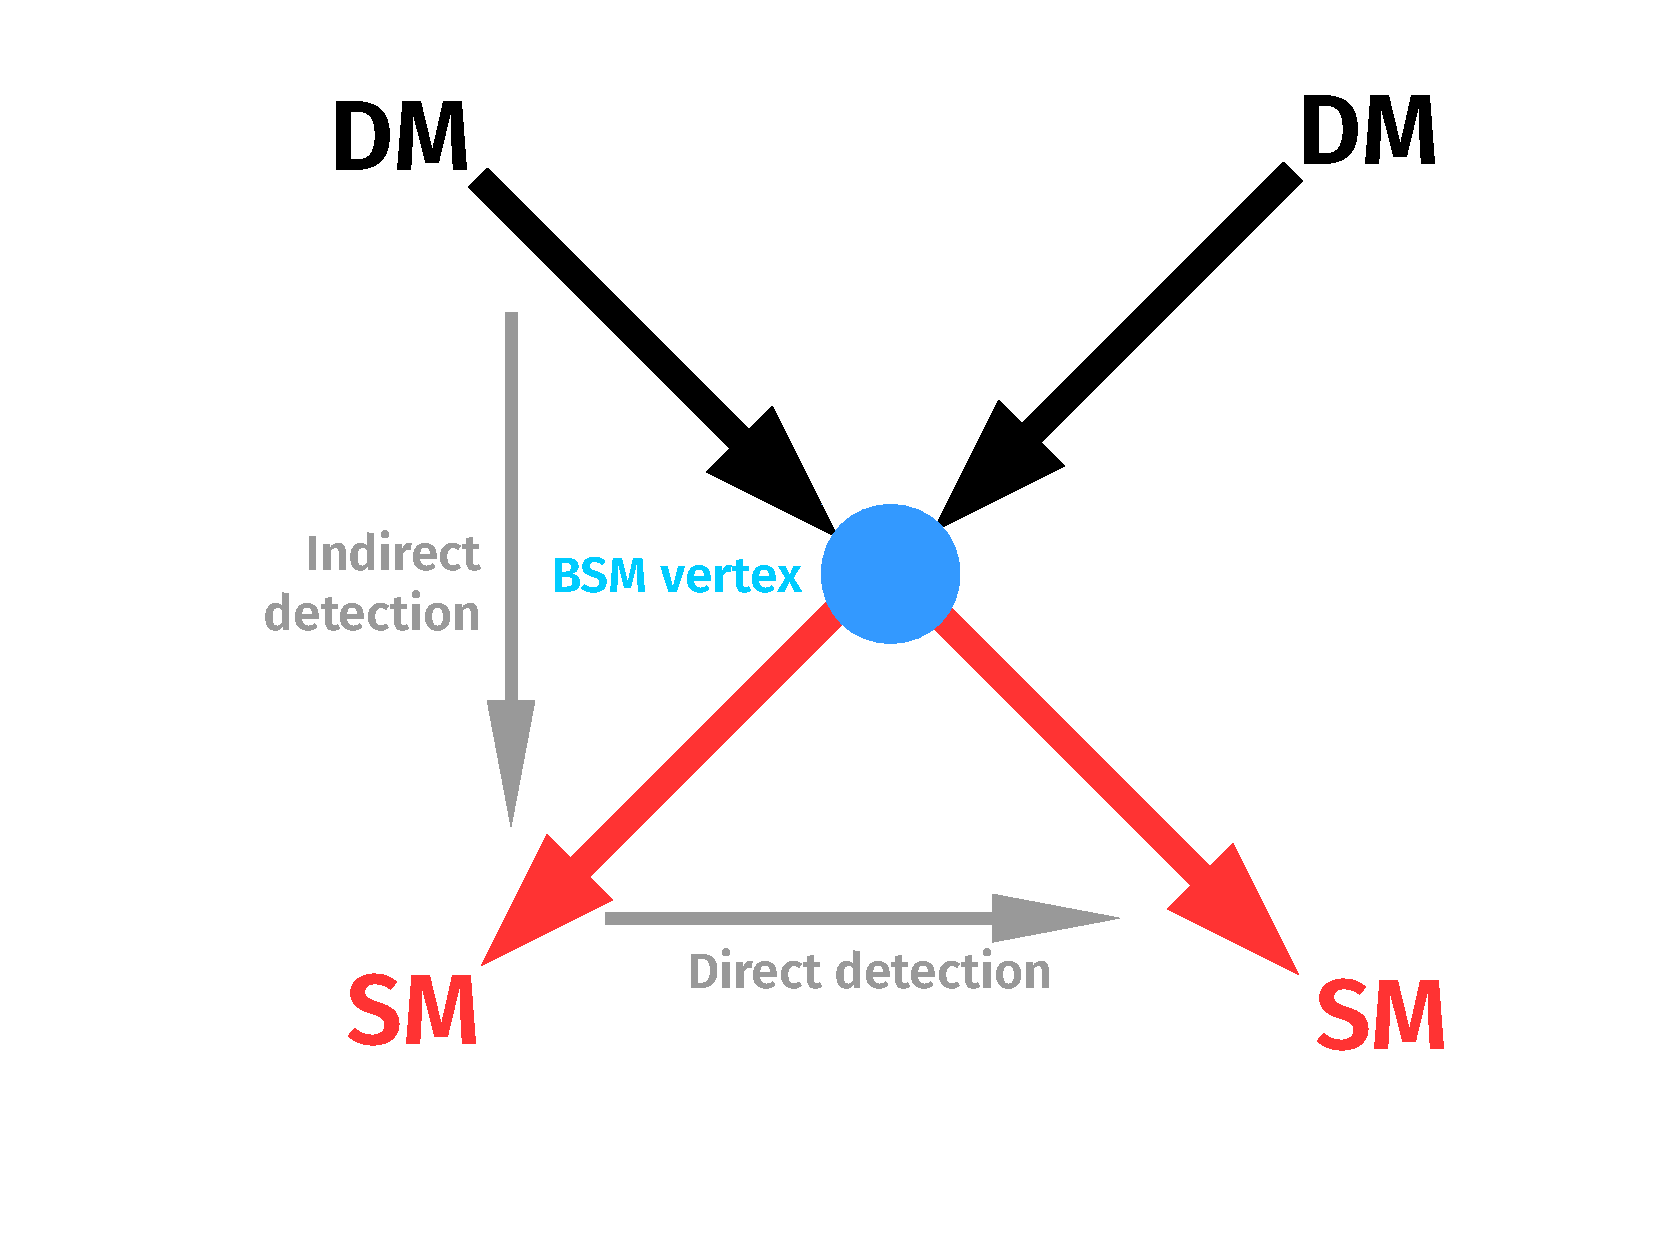
\includegraphics[width=\textwidth]{../figures/talk/id.pdf} \\ 
                  Look for SM remnants of DM-DM annihilation in space }
        \only<3>{ 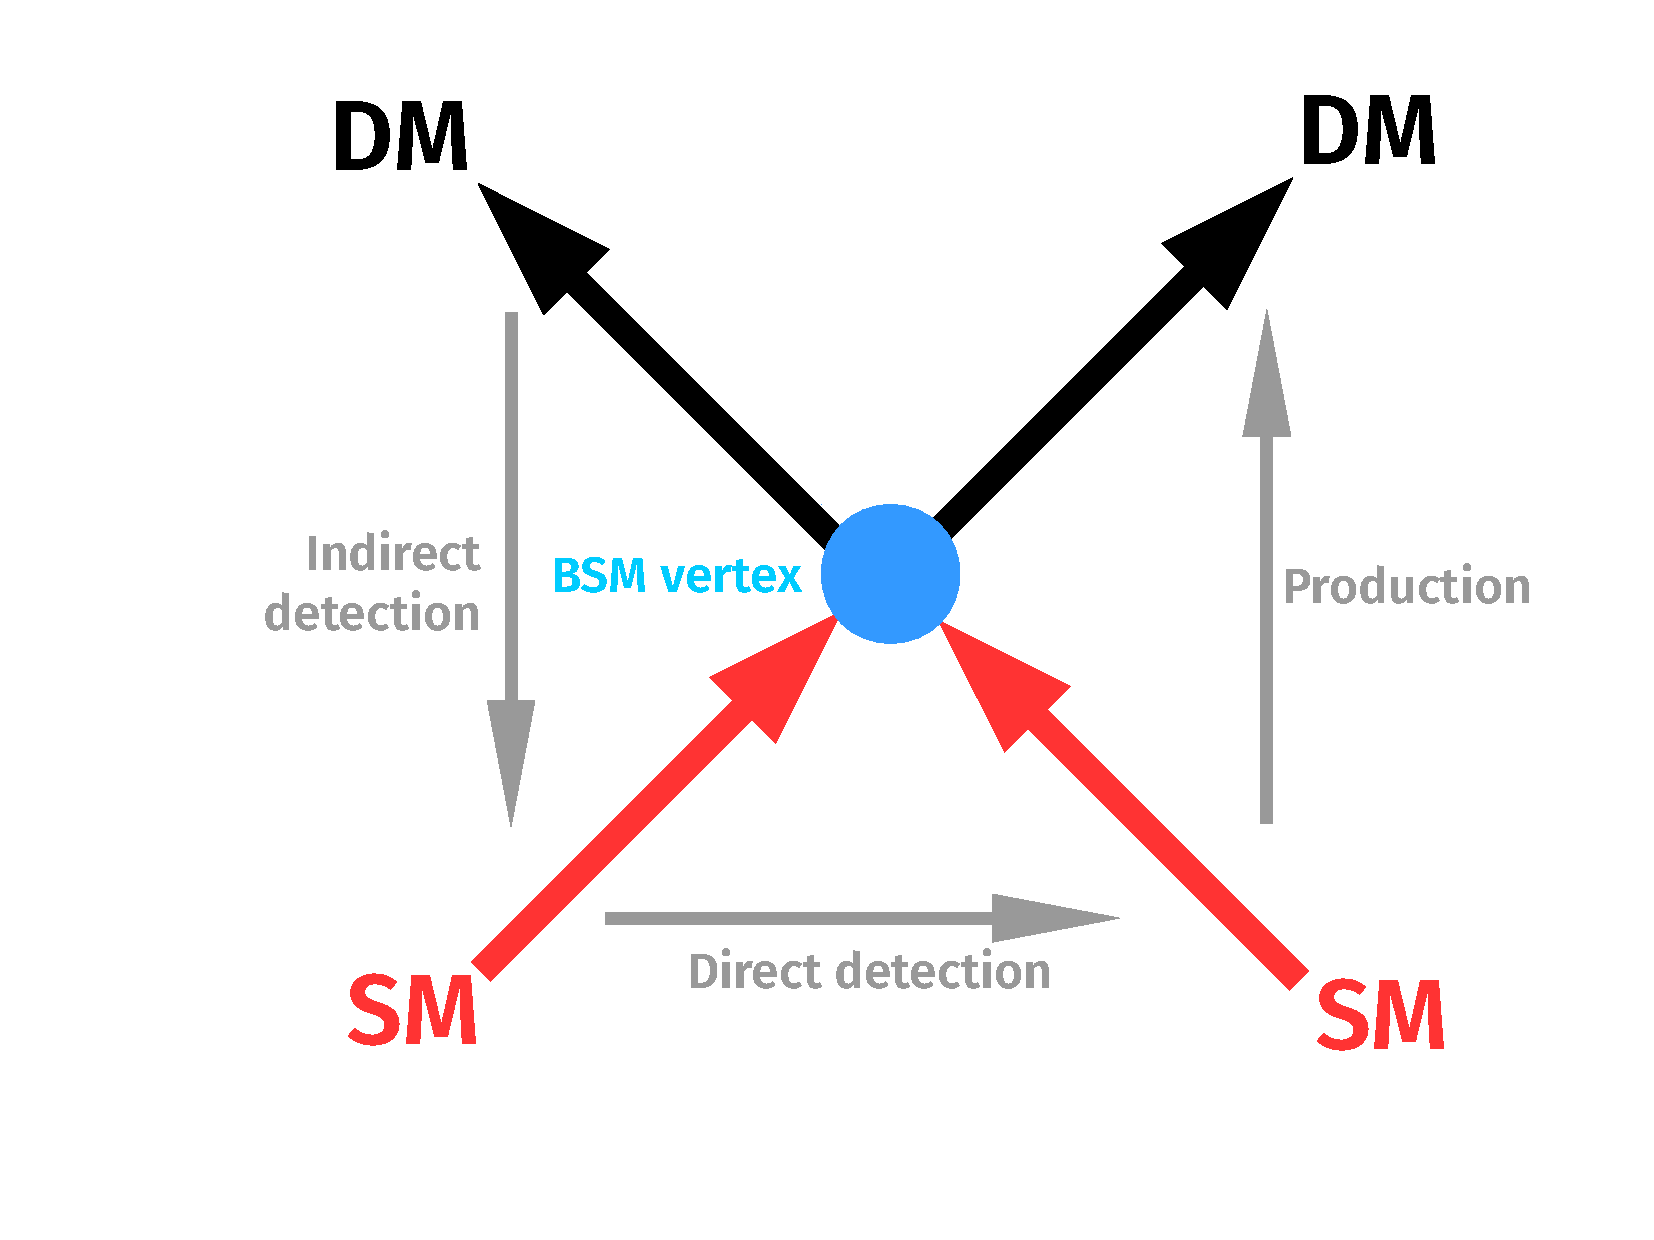
\includegraphics[width=\textwidth]{../figures/talk/lhc.pdf} \\ 
                  Exploit DM-SM interaction to produce DM in a laboratory }
      \end{center}
    \end{column}
    \begin{column}{0.5\textwidth}
      \begin{center}
        \only<1>{ 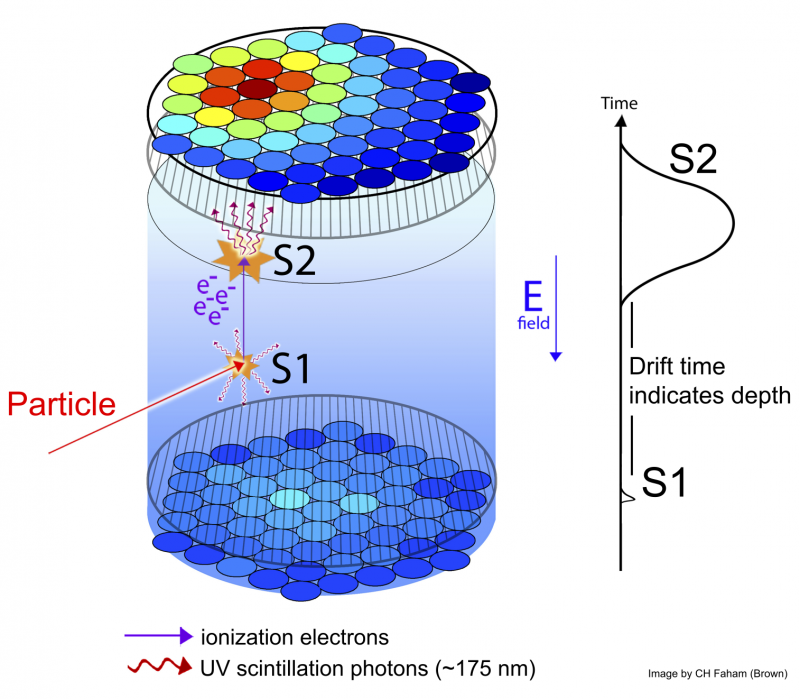
\includegraphics[width=0.9\textwidth]{../figures/talk/lux.png} \mycite{6} \\ 
                  LUX (shown), PandaX, CDMS, Xenon1T,\dots}
        \only<2>{ 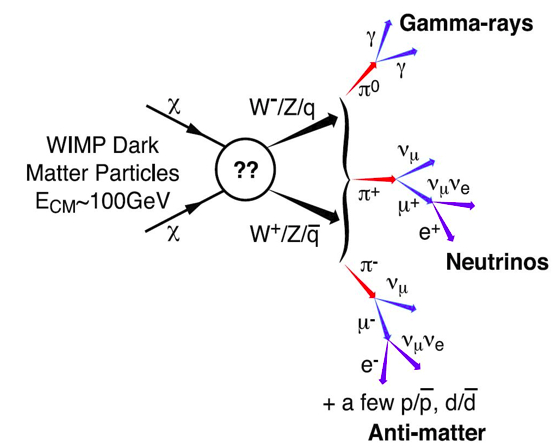
\includegraphics[width=0.9\textwidth]{../figures/talk/fermilat1.png} \mycite{7} \\
                   FermiLAT, AMS}
        \only<3>{ 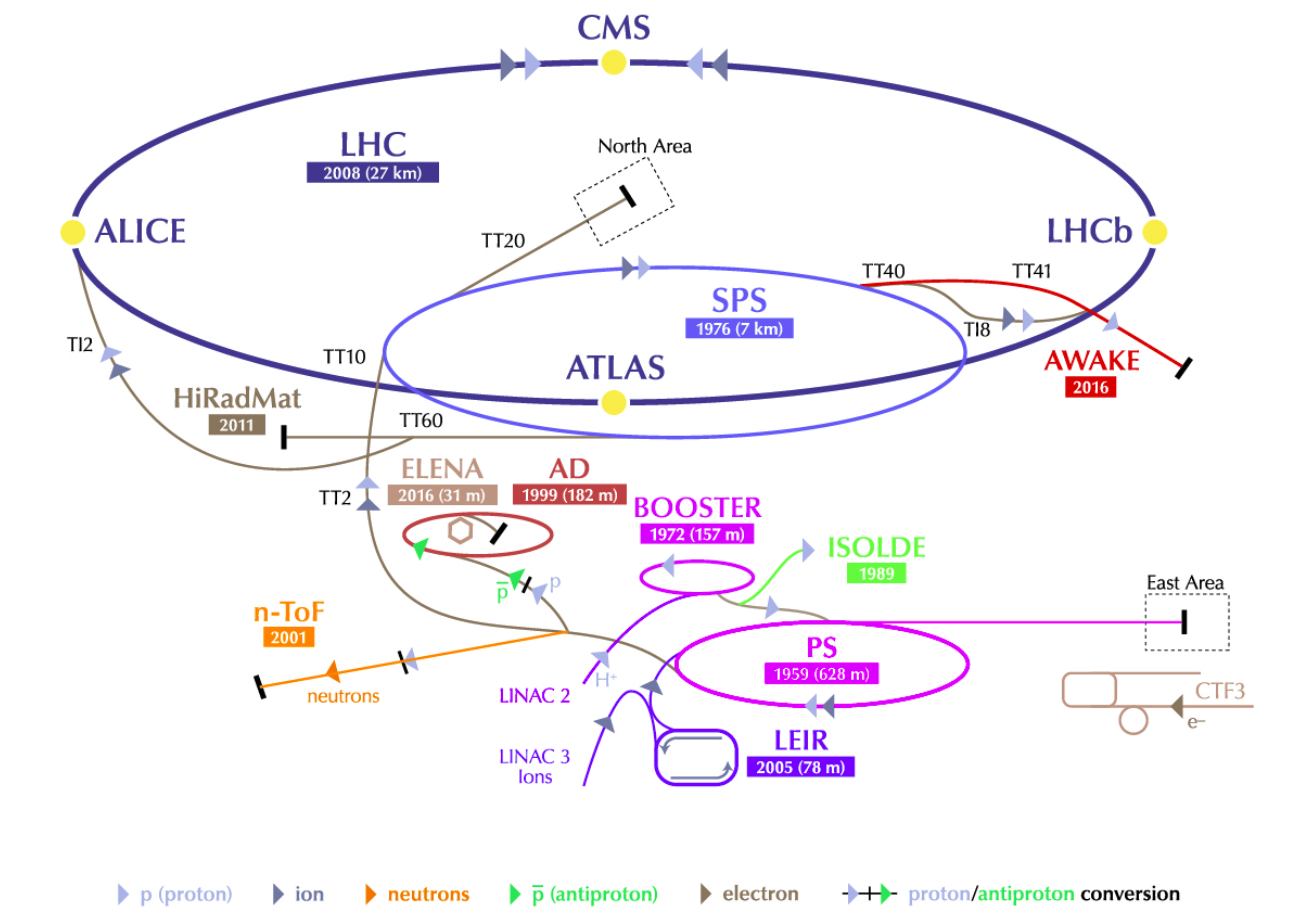
\includegraphics[width=\textwidth]{../figures/cms/lhc.png} }
      \end{center}
    \end{column}
  \end{columns}
\end{frame}

\begin{frame} \frametitle{Production of WIMPs at a hadron collider}
  \vspace{-5mm}
  \centering 
     Effective coupling to quarks/gluons $\gtrsim 10^{-4}$ \hspace{20mm}
    Masses $\lesssim \sqrt{s}$ \\ 
    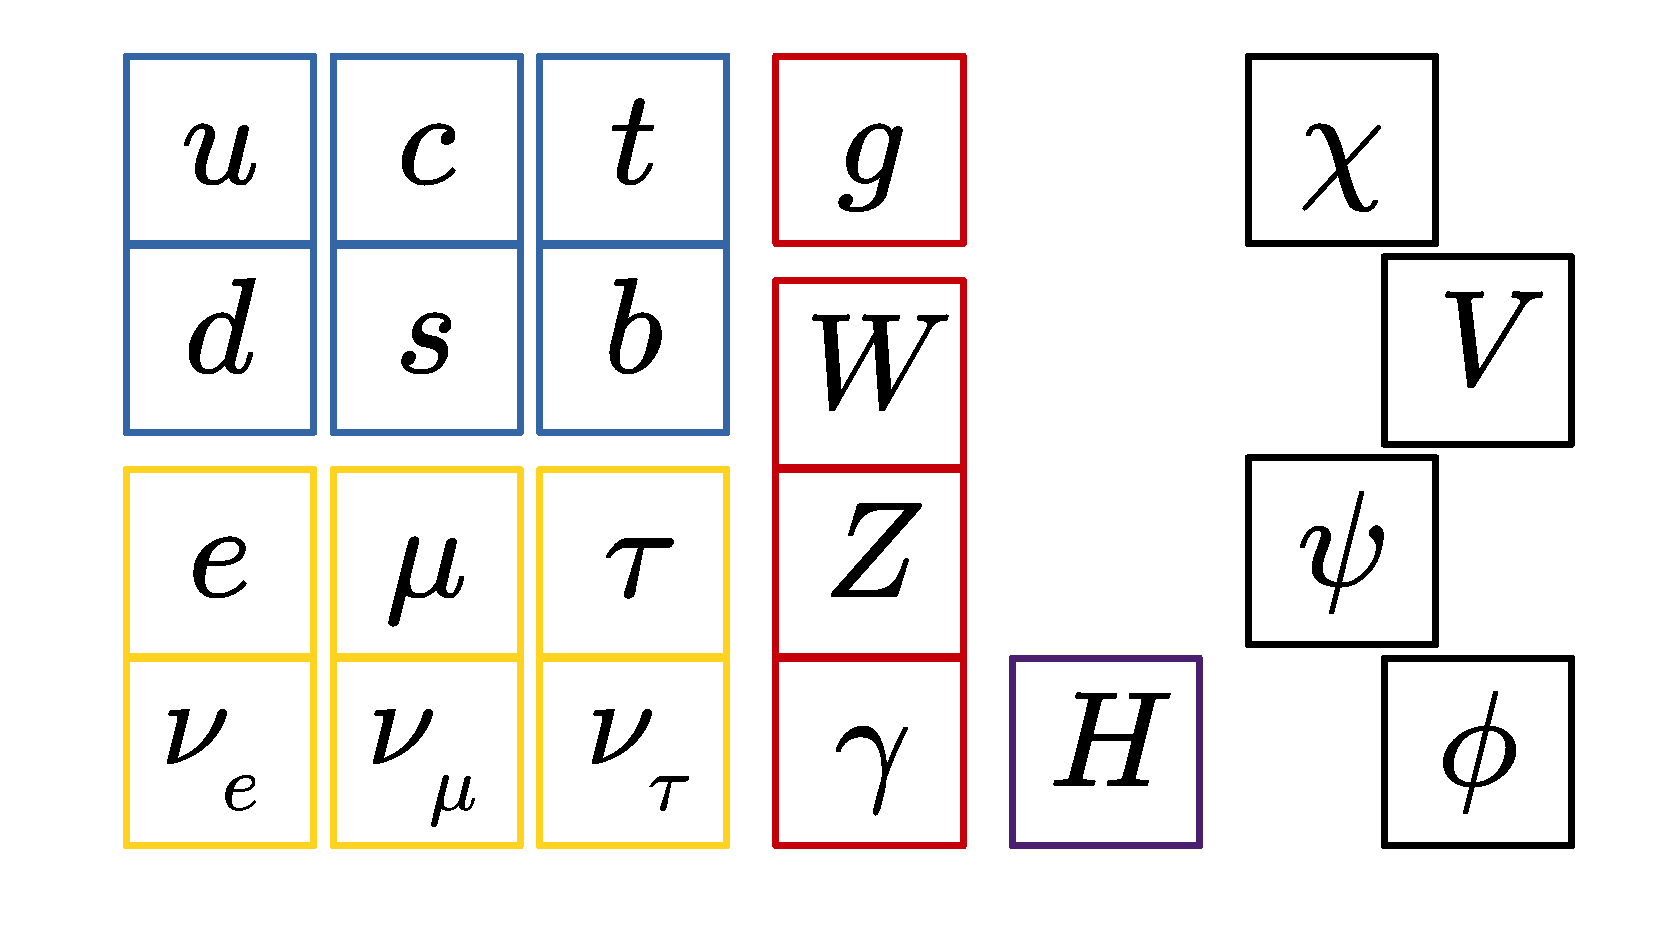
\includegraphics[width=0.8\textwidth]{../figures/talk/dm_fields.pdf}
\end{frame}

\begin{frame} \frametitle{Seeing the invisible at a hadron collider}
  \vspace{-5mm}
  \begin{columns}[T]
    \begin{column}{0.7\textwidth}
    \begin{itemize}
      \item By definition, DM will not interact with a detector 
      \item Look for production of DM with SM particle(s)
      \item Key observable is transverse momentum imbalance
    \end{itemize}
    \end{column}
    \begin{column}{0.3\textwidth}
      \centering
        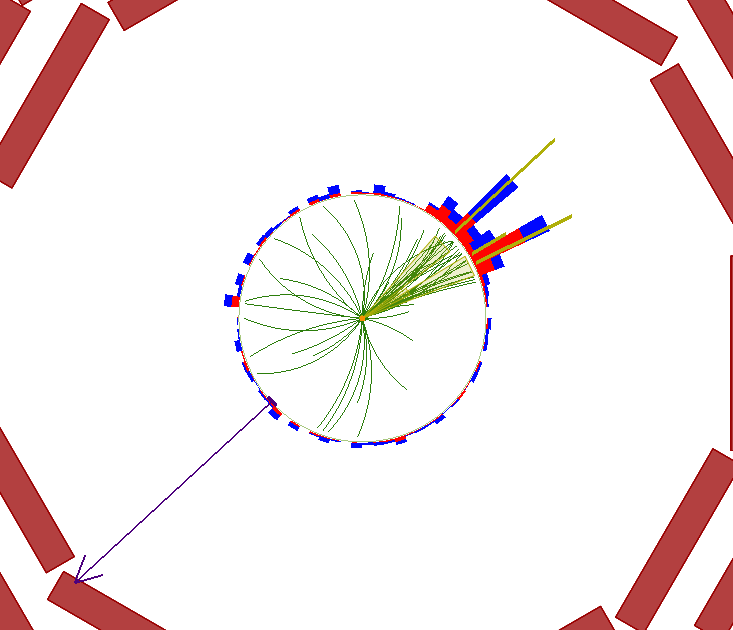
\includegraphics[width=0.8\textwidth]{../figures/talk/1275337_634520340_334_RhoPhi.png}
    \end{column}
  \end{columns}
  \begin{columns}
    \begin{column}{0.6\textwidth}
      \vspace{-10mm}
      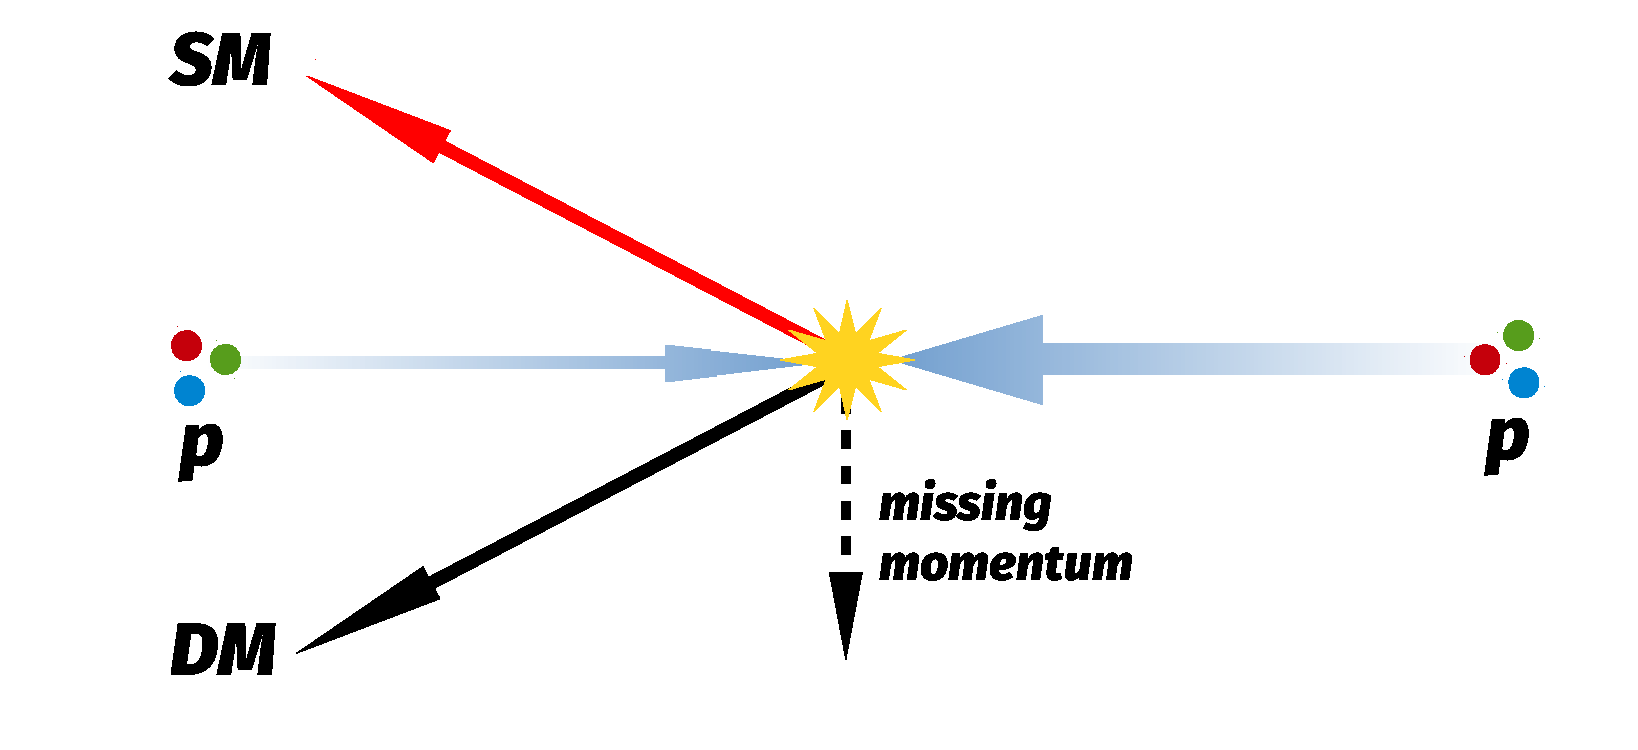
\includegraphics[width=\textwidth]{../figures/talk/ptmiss3.pdf}
    \end{column}
    \begin{column}{0.4\textwidth}
      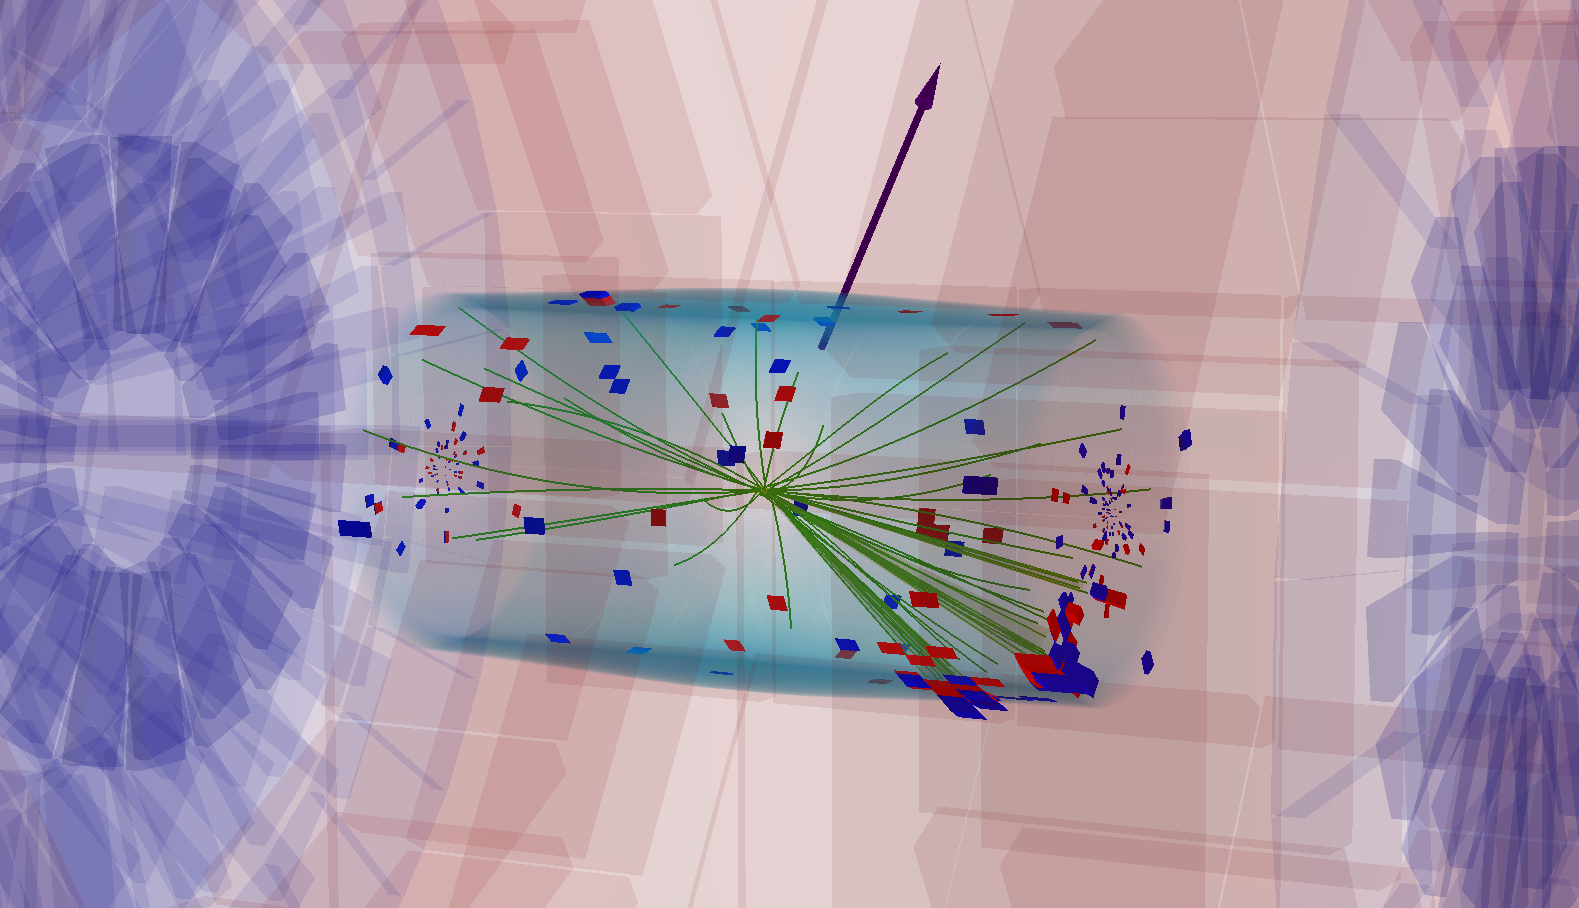
\includegraphics[width=\textwidth]{../figures/talk/1275337_634520340_334_3DTower2.png}
    \end{column}
  \end{columns}
\end{frame}

\begin{frame}[t]   \frametitle{Which SM particle(s)?}
  \vspace{-3mm}
  \centering
  Many to choose from. SM particle choice $\Leftrightarrow$ type of DM you can look for\\
  \vspace{3mm}
  \begin{tabular}{r|c||c|c|c|c|c}
                    & SM particle & \mlc{Minimal\\extension} & \mlc{Higgs-\\like} & \mlc{Extra\\dimensions}    & \mlc{Extended\\Higgs sector} & \mlc{Flavor\\violation}\\
     \hline
     \hline
    \multirow{5}{*}{Quarks} &
    $q(g)$          &  \rc                    &     \rc                 &   \rc                     &                        &  \\
  &    $t$             &  \drc                    &                         &                           &                    &    \drc    \\
  &    $qq'$           &                         &     \drc                 &                           &                      &      \\
  &    $t\bar{t}$      &                         &     \rc                 &                           &                       &     \\
  &    $b/b\bar{b}$    &                         &     \rc                 &                           &                        & \rc   \\ \hline
  \multirow{3}{*}{Gauge bosons} &
    $\gamma$        &  \rc                    &                         &  \rc                      &                      &      \\
  &$V\rightarrow q\bar{q}'$
                    &  \rc                    &     \rc                 &                           &                     &     \\
  &  $Z\rightarrow\ell^+\ell^-$
                    &  \rc                    &     \rc                 & \rc                       &                       &     \\ \hline
  Higgs & $H\rightarrow x\bar{x}$
                    &                         &                         &                           & \rc                    &   \\
  \end{tabular}
\end{frame}


\begin{frame}[t]  \frametitle{$\ptmiss$ at the LHC}
  \vspace{-7mm}
  \begin{columns}[T]
  \begin{column}{0.4\textwidth}
    \begin{itemize}
      \item CMS records collisions from the LHC
      \begin{itemize}
        \item Today: $\sqrt{s}=13$\,TeV $pp$ collision data from 2016
      \end{itemize}
    \item Missing momentum:
        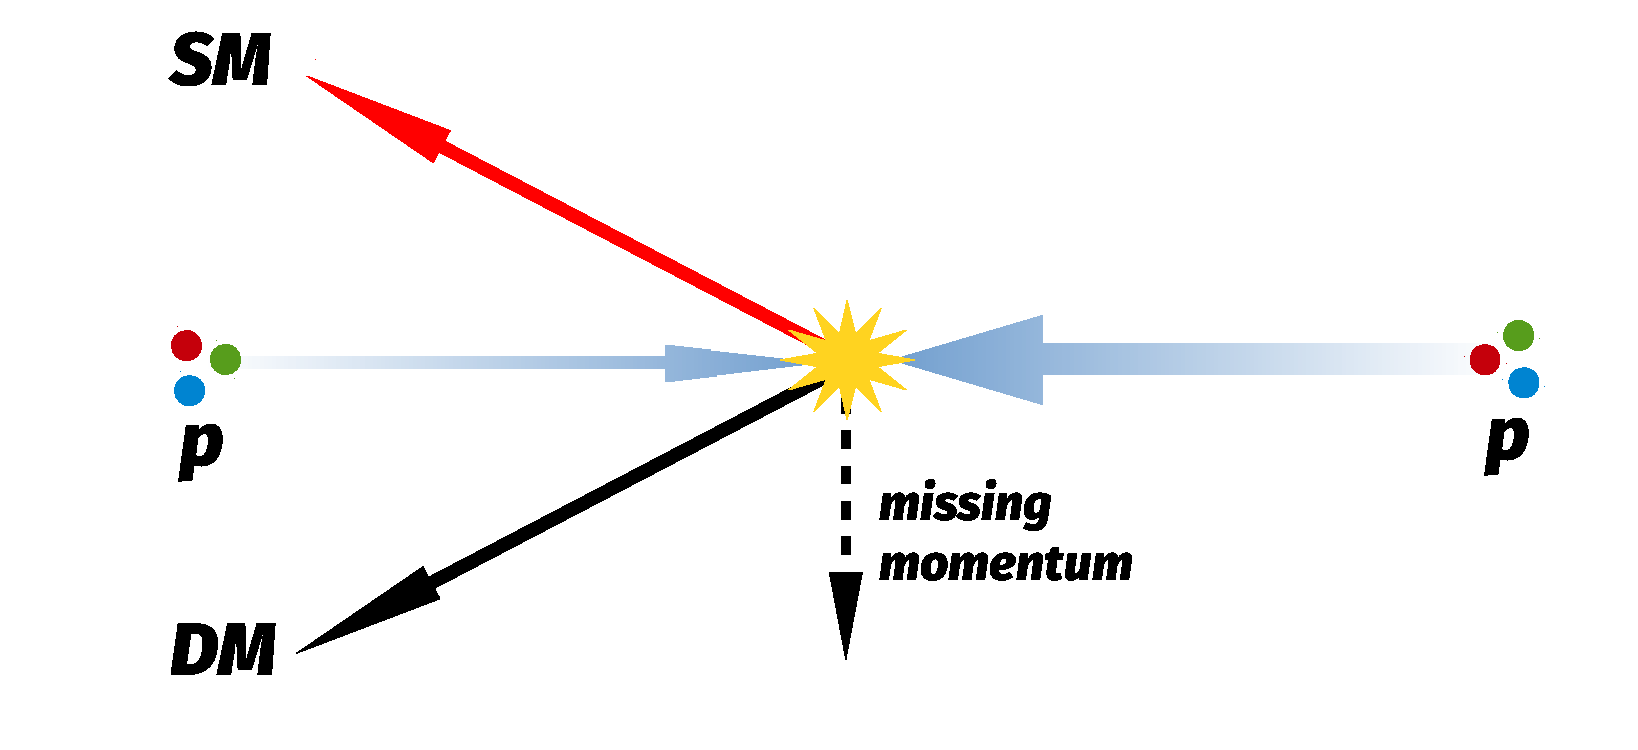
\includegraphics[width=0.8\textwidth]{../figures/talk/ptmiss3.pdf}
      \uncover<2->{
      \item turns into:
        \[\vec{p}_\mathrm{T}^\mathrm{\,miss} = -\sum_{i\in\mathrm{particles}} \vec{p}_{\mathrm{T},i}\]
      }
    \end{itemize}
  \end{column}
  \begin{column}{0.6\textwidth}
    \centering
    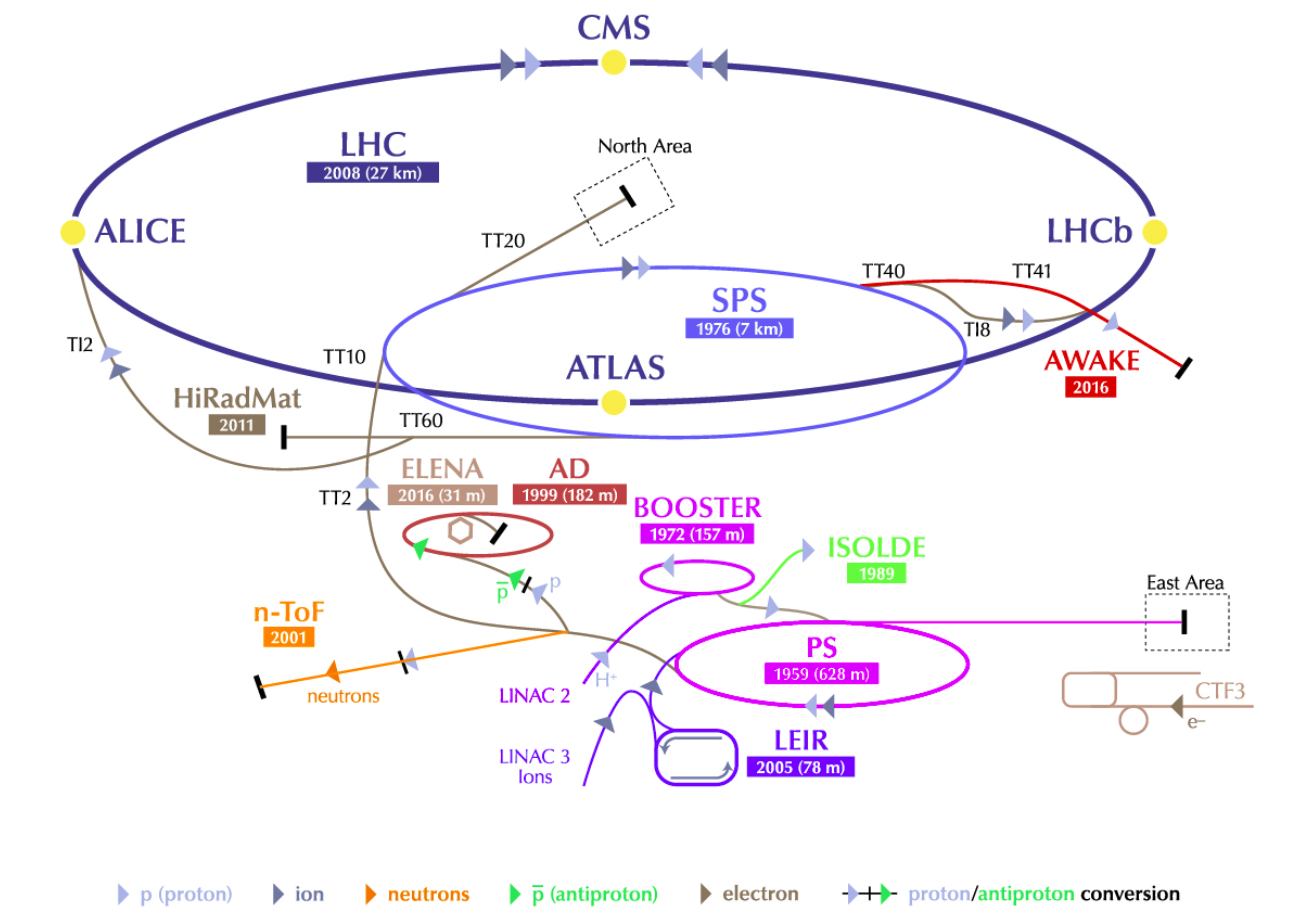
\includegraphics[width=\textwidth]{../figures/cms/lhc.png} \\
    \vspace{-35mm}\hspace{10mm}
    \uncover<2->{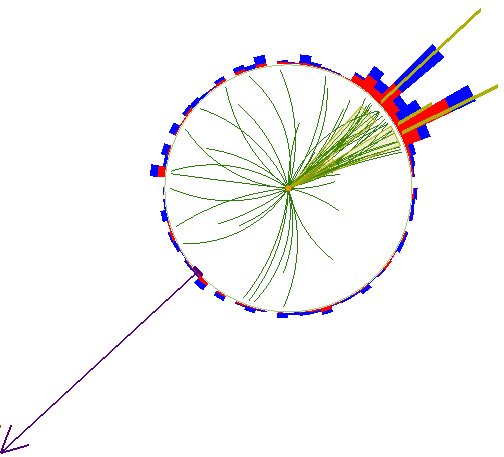
\includegraphics[width=0.6\textwidth]{../figures/talk/1275337_634520340_334_RhoPhi2.png}}
  \end{column}
  \end{columns}
\end{frame}

\begin{frame} \frametitle{Proton collisions}
  \vspace{-5mm}
  \begin{columns}
    \begin{column}{0.4\textwidth}
      \begin{itemize}
        \item Two 6.5 TeV proton beams
        \item $\sim 10^{11}$ protons per bunch
        \item Average collision has 10-25 pile-up interactions 
      \end{itemize}
      \centering 
      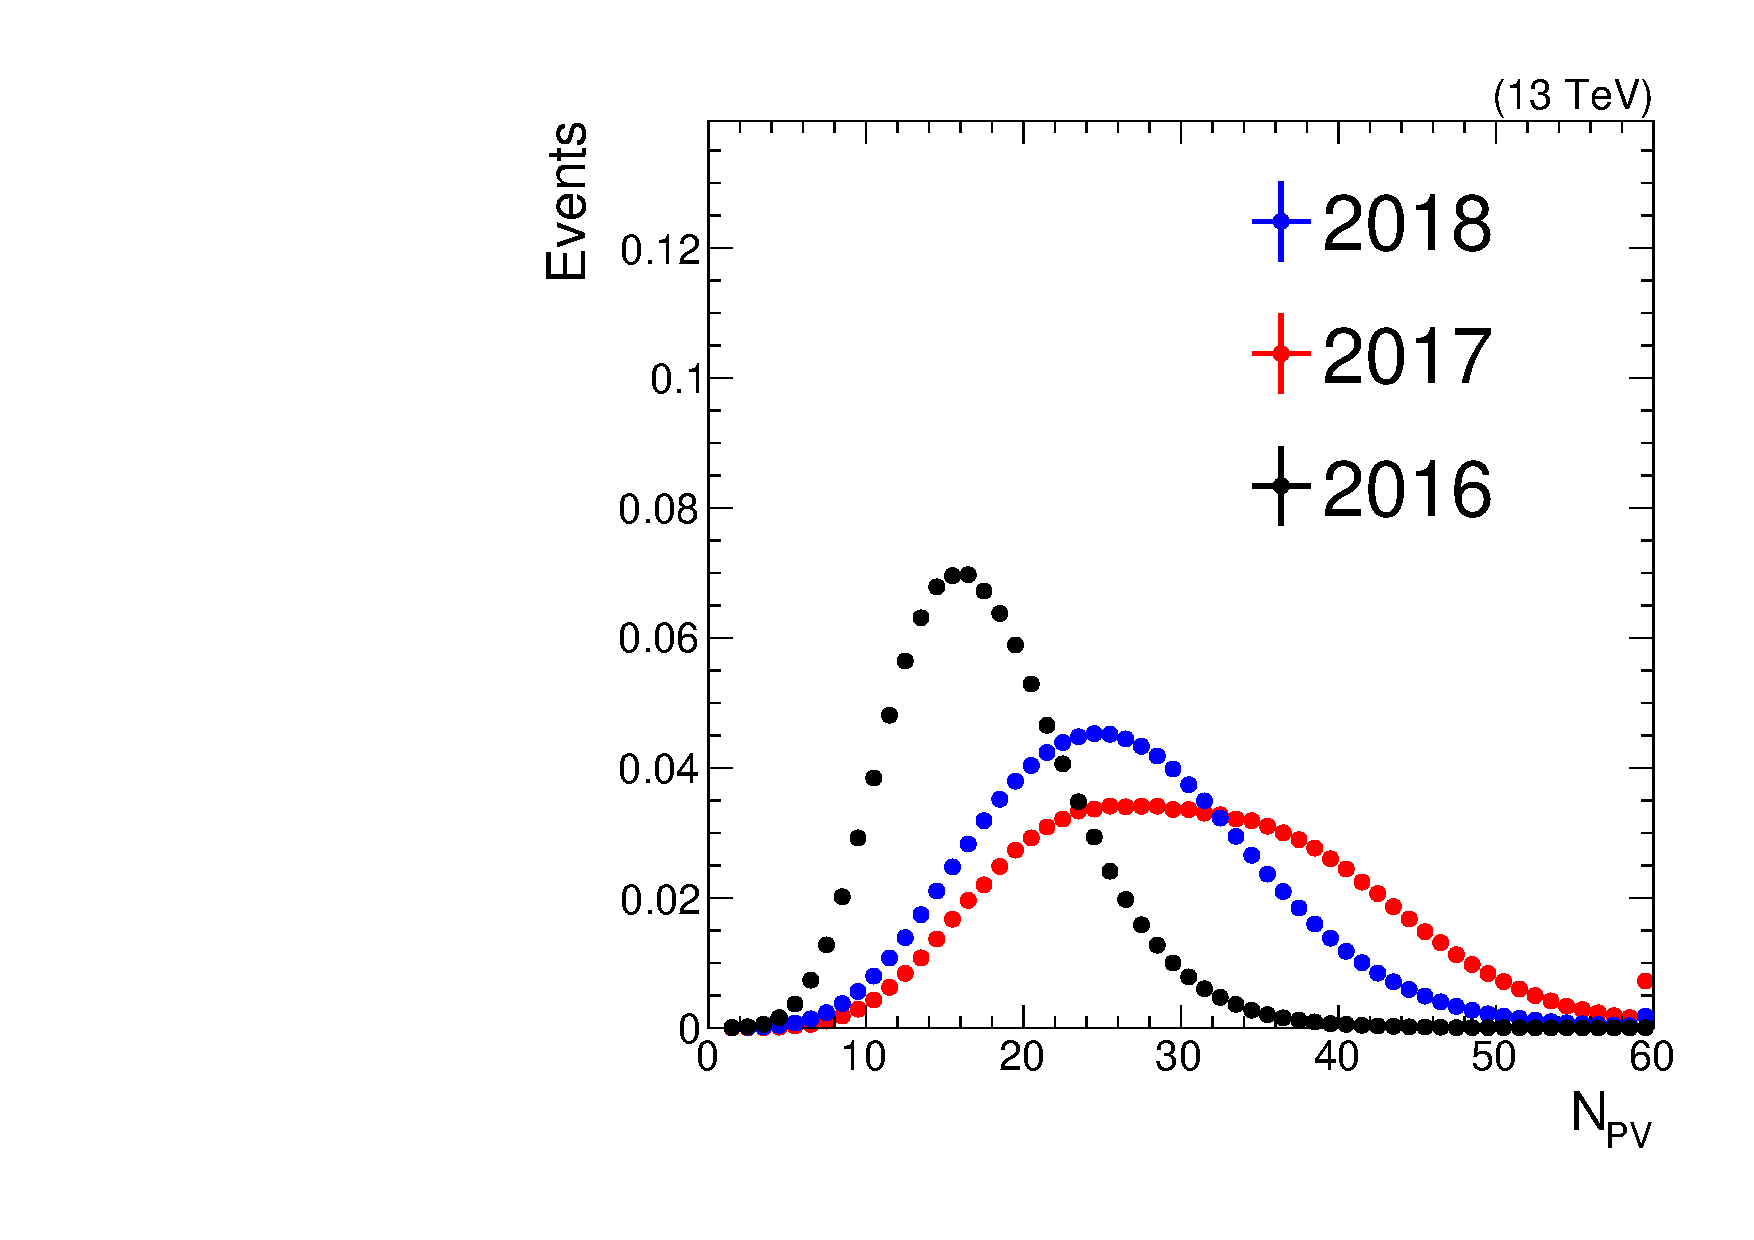
\includegraphics[width=0.75\textwidth]{../figures/cms/comparison_npv.pdf}
    \end{column}
    \begin{column}{0.6\textwidth}
      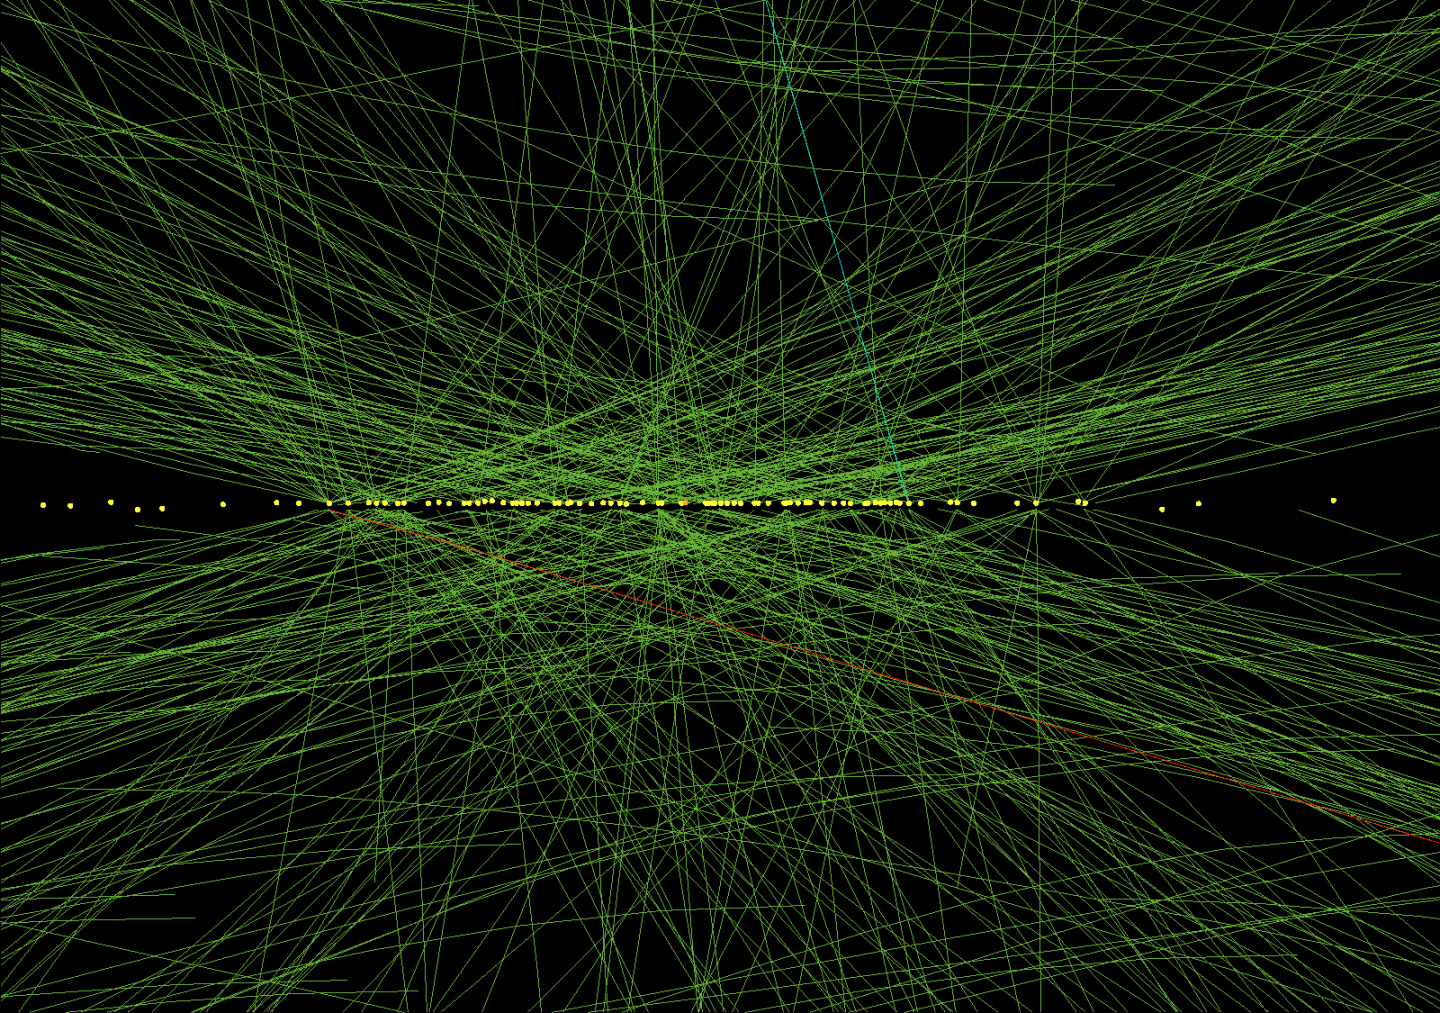
\includegraphics[width=\textwidth]{../figures/talk/vertices.png}
    \end{column}
  \end{columns}
\end{frame}

\begin{frame}[t]   \frametitle{Compact Muon Solenoid}
  \vspace{-5mm}
  \begin{columns}[T]
  \begin{column}{0.4\textwidth}
    All particles in sum $\Rightarrow$ \\
    all subdetectors help measure $\ptmiss$!
  \vspace{-3mm}
  \begin{itemize}
        \item Solenoidal magnet
        \begin{itemize}
          \item $3.8\,$T B field
        \end{itemize}
        \item Silicon tracker
        \begin{itemize}
          \item Charged particles' $\vec{p}$
          \item Track vertices
        \end{itemize}
        \item Calorimeters
        \begin{itemize}
          \item EM and hadronic
          \item Good energy resolution
          \item Large coverage
        \end{itemize}
        \item Muon chambers
        \begin{itemize}
          \item ID muons
          \item Help measure $\vec{p}$
        \end{itemize}
  \end{itemize}
  \end{column}
  \begin{column}{0.6\textwidth}
    \centering
    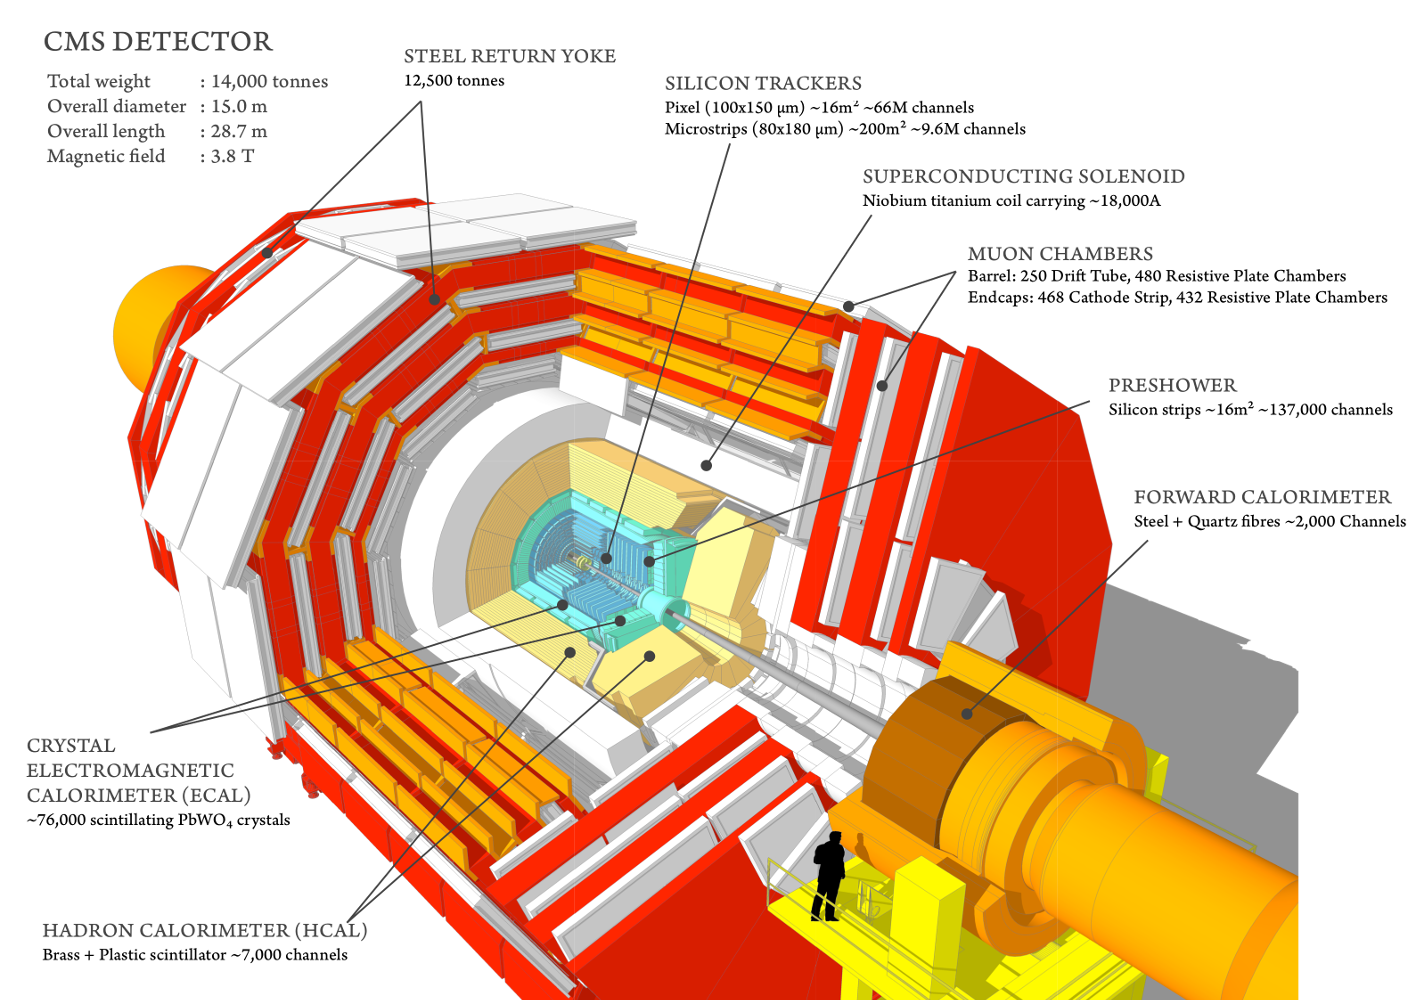
\includegraphics[width=\textwidth]{../figures/talk/cms.png}
  \end{column}
  \end{columns}
\end{frame}

\begin{frame} \frametitle{Particle reconstruction}
  \vspace{-7mm}
  \centering 
  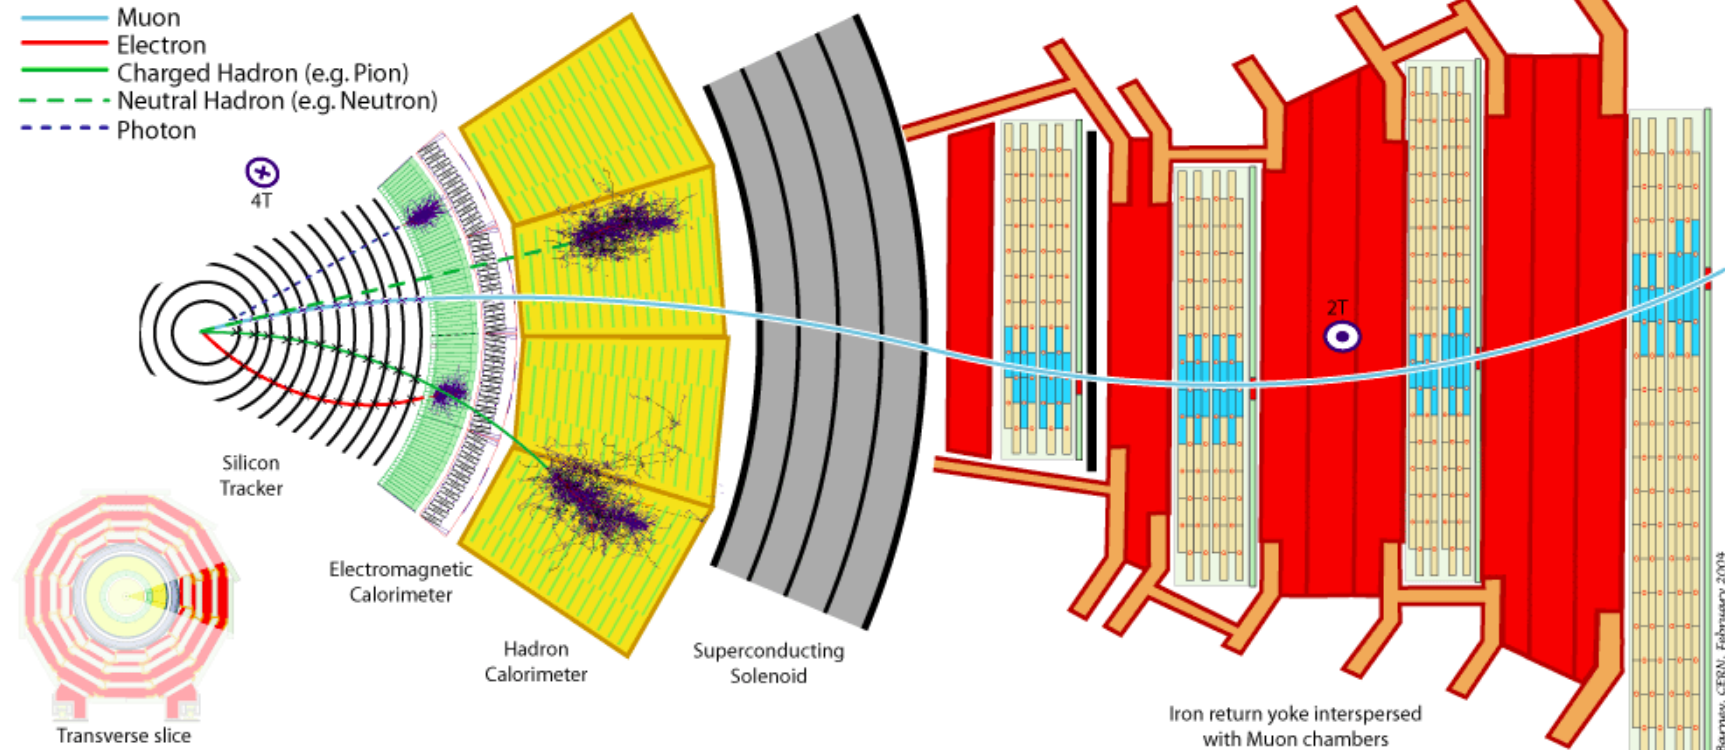
\includegraphics[width=0.8\textwidth]{../figures/talk/cms_transverse.png}\mycite{8} \\ 
  \begin{tabular}{c|c|c|c}
    Tracker & ECAL & HCAL & Muon \\ 
     \hline 
     \hline 
     $|\eta|<2.5$ & $|\eta| <3$ & $|\eta|<5$ & $|\eta|<2.4$ \\ 
     $\frac{0.015\%\cdot\pt}{\mathrm{GeV}} \oplus 0.5\%$ &
     $\frac{3\%}{\sqrt{\nicefrac{E}{\mathrm{GeV}}}} \oplus \frac{12\%}{E/\mathrm{GeV}} \oplus 0.3\%$ & 
     $\frac{85\%}{\sqrt{\nicefrac{E}{\mathrm{GeV}}}} \oplus 7.4\%$ &
     $3\%$ at 100 GeV \\ 
  \end{tabular}
\end{frame}


\begin{frame}  \frametitle{Outline of this talk}
  \vspace{-5mm}
  \begin{columns}[T]
    \begin{column}{0.5\textwidth}
      \centering
      \mlink{DM production mode}
    \end{column}
    \begin{column}{0.5\textwidth}
      \centering
      \mlink{Highlights}
    \end{column}
  \end{columns}
  \begin{columns}
    \begin{column}{0.5\textwidth}
      \begin{center}
        Top quark + DM \\ 
        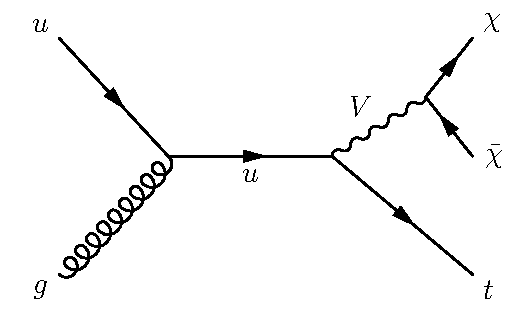
\includegraphics[width=0.49\textwidth]{../figures/monotop/diagrams/fcncb.pdf}
        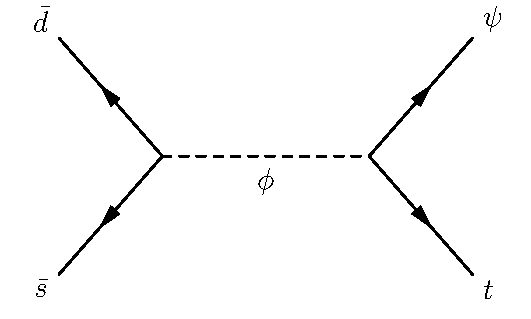
\includegraphics[width=0.49\textwidth]{../figures/monotop/diagrams/resonant.pdf}
      \end{center}
      \pause
    \end{column}
    \begin{column}{0.5\textwidth}
      \centering
      Jet substructure
      \\ Invisible background estimation
    \end{column}
  \end{columns}
  \pause
  \begin{columns}
    \begin{column}{0.5\textwidth}
      \begin{center}
        Higgs $\rightarrow$ DM \\ 
        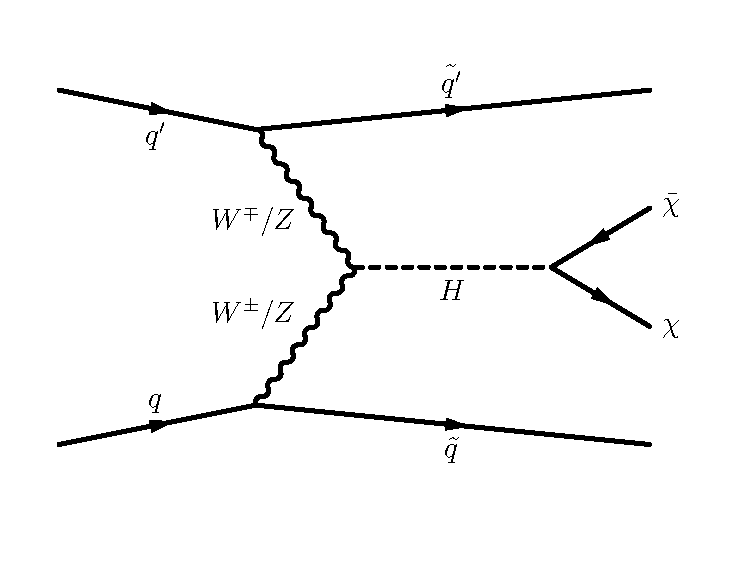
\includegraphics[width=0.49\textwidth]{../figures/vbf/diagrams/vbf_hinv.pdf}
      \end{center}
      \pause
    \end{column}
    \begin{column}{0.5\textwidth}
      \centering
      Forward jets \\
      Electroweak SM backgrounds 
    \end{column}
  \end{columns}
\end{frame}

\secpage{Mono-Top}

\begin{frame}[t]  \frametitle{Hallmarks of top quark$+\ptmiss$}
  \vspace{-5mm}
  \begin{columns}[T]
  \begin{column}{0.65\textwidth}
  \begin{itemize}
    \uncover<1->{
      \item Final state violates flavor conservation
      \begin{itemize}
        \item { SM will have $b$ quark in the final state}
      \end{itemize}
      \item { Excess mono-top production $\Rightarrow$ flavor-changing BSM }
    }
    \uncover<2->{
      \item Leading SM process: 0.14 pb $\Rightarrow$ 5000 events in 36/fb 
    }
  \end{itemize}
    \uncover<2->{
      \begin{center}
        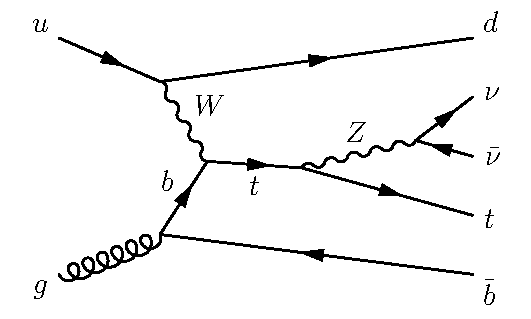
\includegraphics[width=0.5\textwidth]{../figures/monotop/diagrams/tzq.pdf}
      \end{center}
    }
  \end{column}
  \begin{column}{0.35\textwidth}
    \uncover<3->{
        \centering
        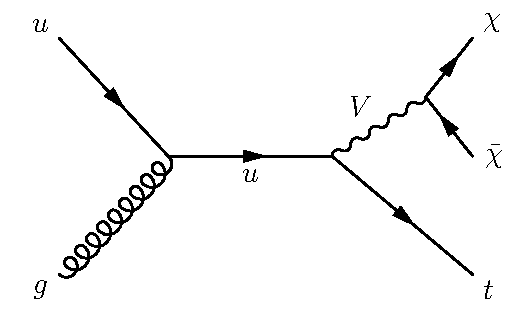
\includegraphics[width=\textwidth]{../figures/monotop/diagrams/fcncb.pdf} \\
        % \vspace{5mm}
        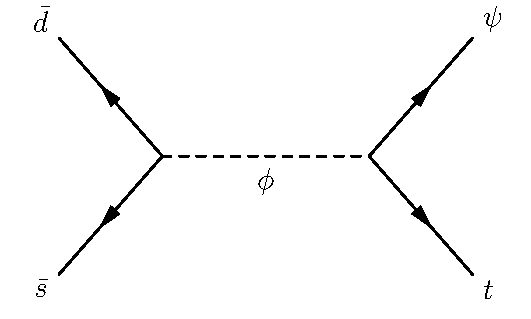
\includegraphics[width=\textwidth]{../figures/monotop/diagrams/resonant.pdf} \\
      }
  \end{column}
  \end{columns}
\end{frame}

\begin{frame}[t] \frametitle{Connection to other DM models}
  \vspace{-5mm}
  \begin{columns}[T]
	\begin{column}{0.5\textwidth}
      \centering 
        Flavor conserving: diagonal $g_u^V$ \\ 
        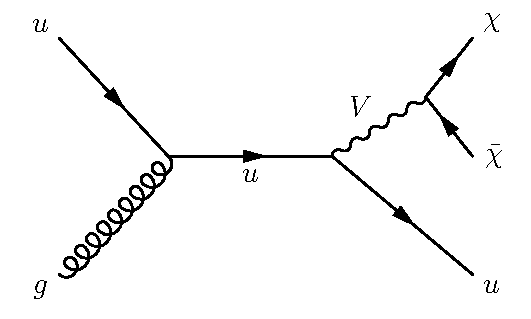
\includegraphics[width=0.6\textwidth]{../figures/monotop/diagrams/mj.pdf} \\ 
        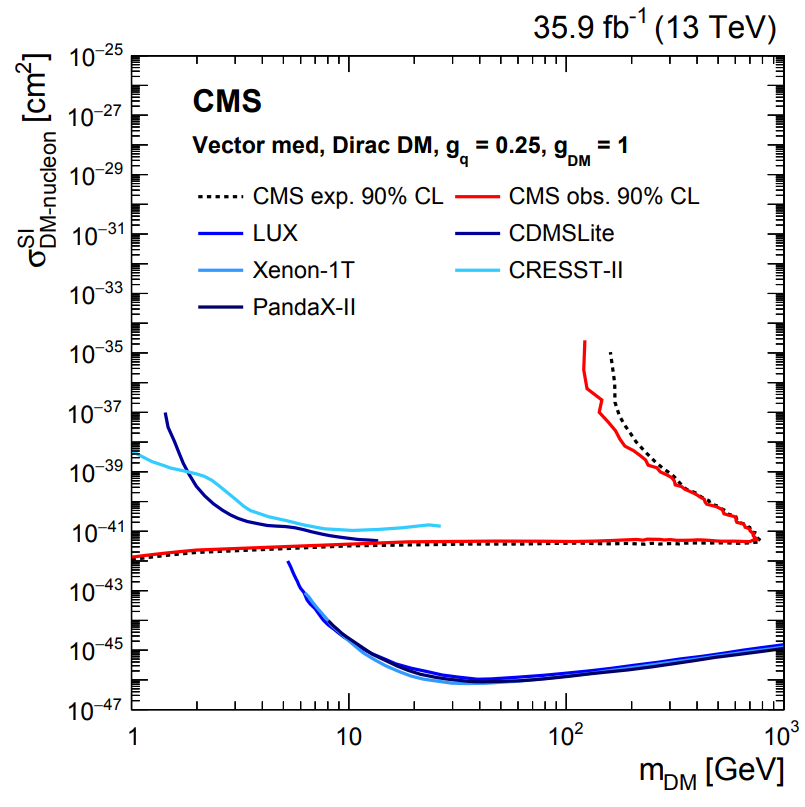
\includegraphics[width=0.45\textwidth]{../figures/talk/monojet.png}
        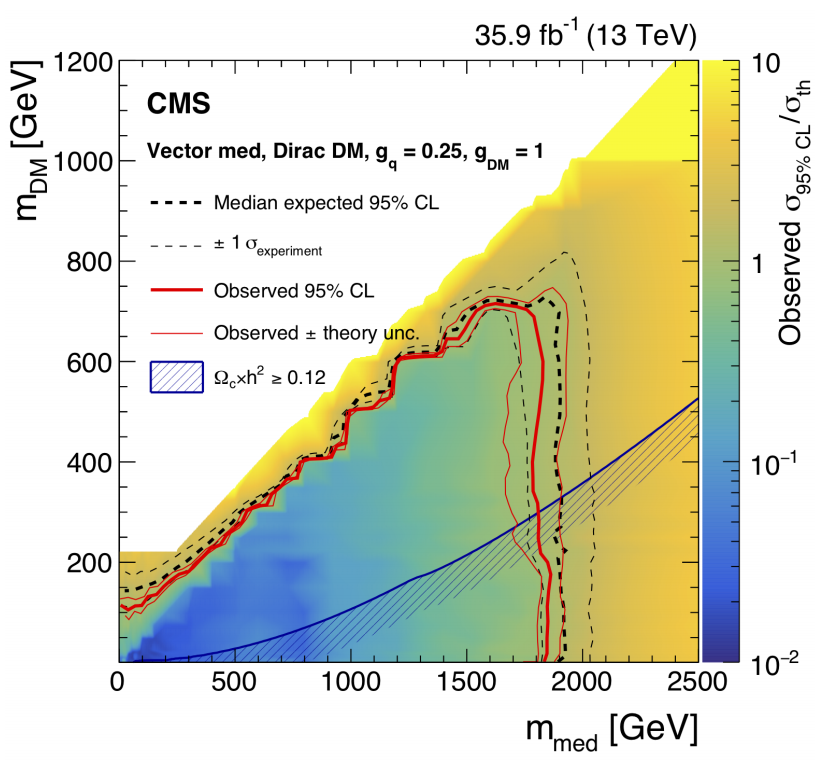
\includegraphics[width=0.5\textwidth]{../figures/talk/monojet2.png}
    \end{column}
	\begin{column}{0.5\textwidth}
      \centering 
        Flavor violating: off-diagonal $g_u^V$ \\ 
        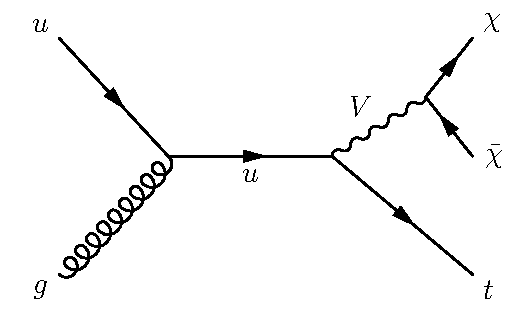
\includegraphics[width=0.6\textwidth]{../figures/monotop/diagrams/fcncb.pdf} \\ 
        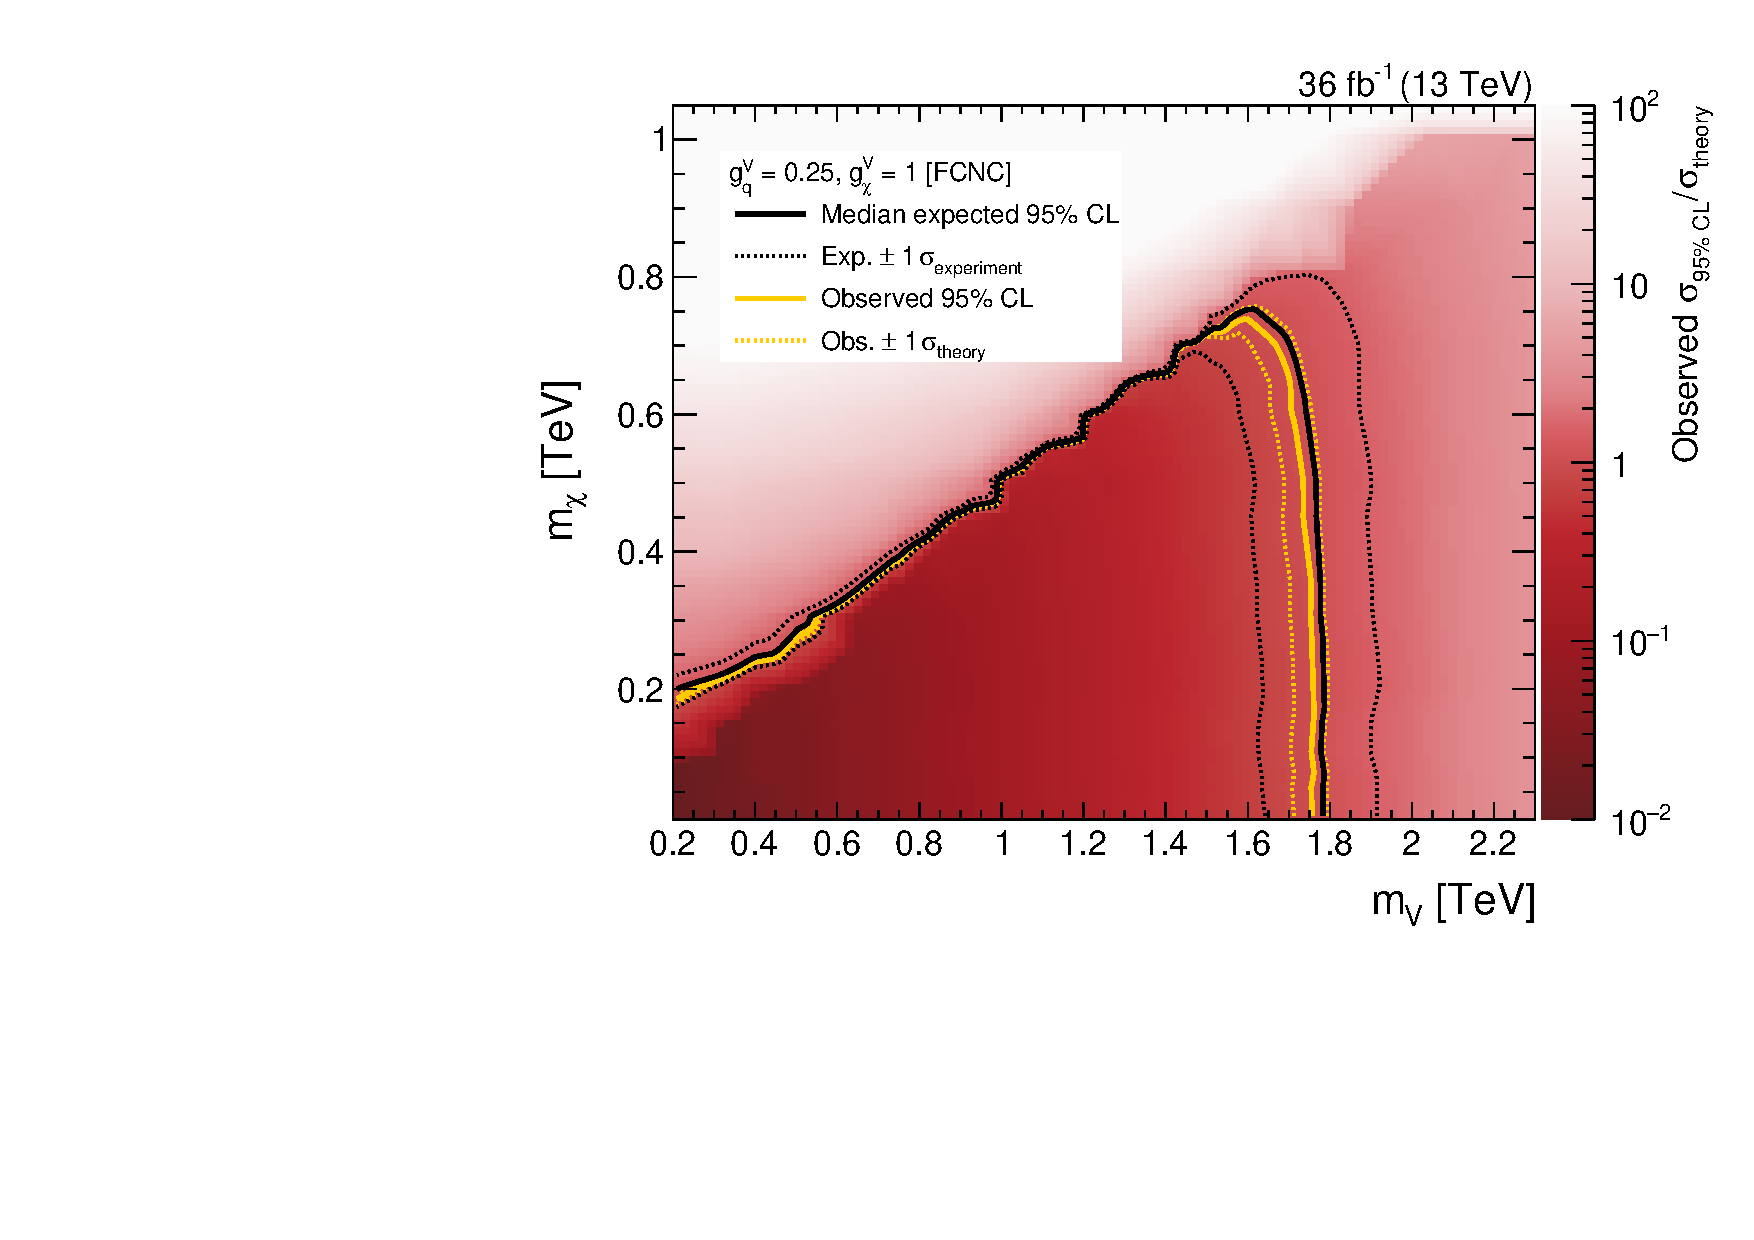
\includegraphics[width=0.6\textwidth]{../figures/monotop/results/fcnc2d_obs_vector.pdf}
    \end{column}
  \end{columns}
\end{frame}

\begin{frame}[t]  \frametitle{Anatomy of a mono-top event}
  \vspace{-7mm}
  \begin{columns}[T]
  \begin{column}{0.45\textwidth}
    \centering
    \only<1>{Hadronic decay $\Rightarrow$ larger $\mathcal{B}$, no $\ptmiss$\\
             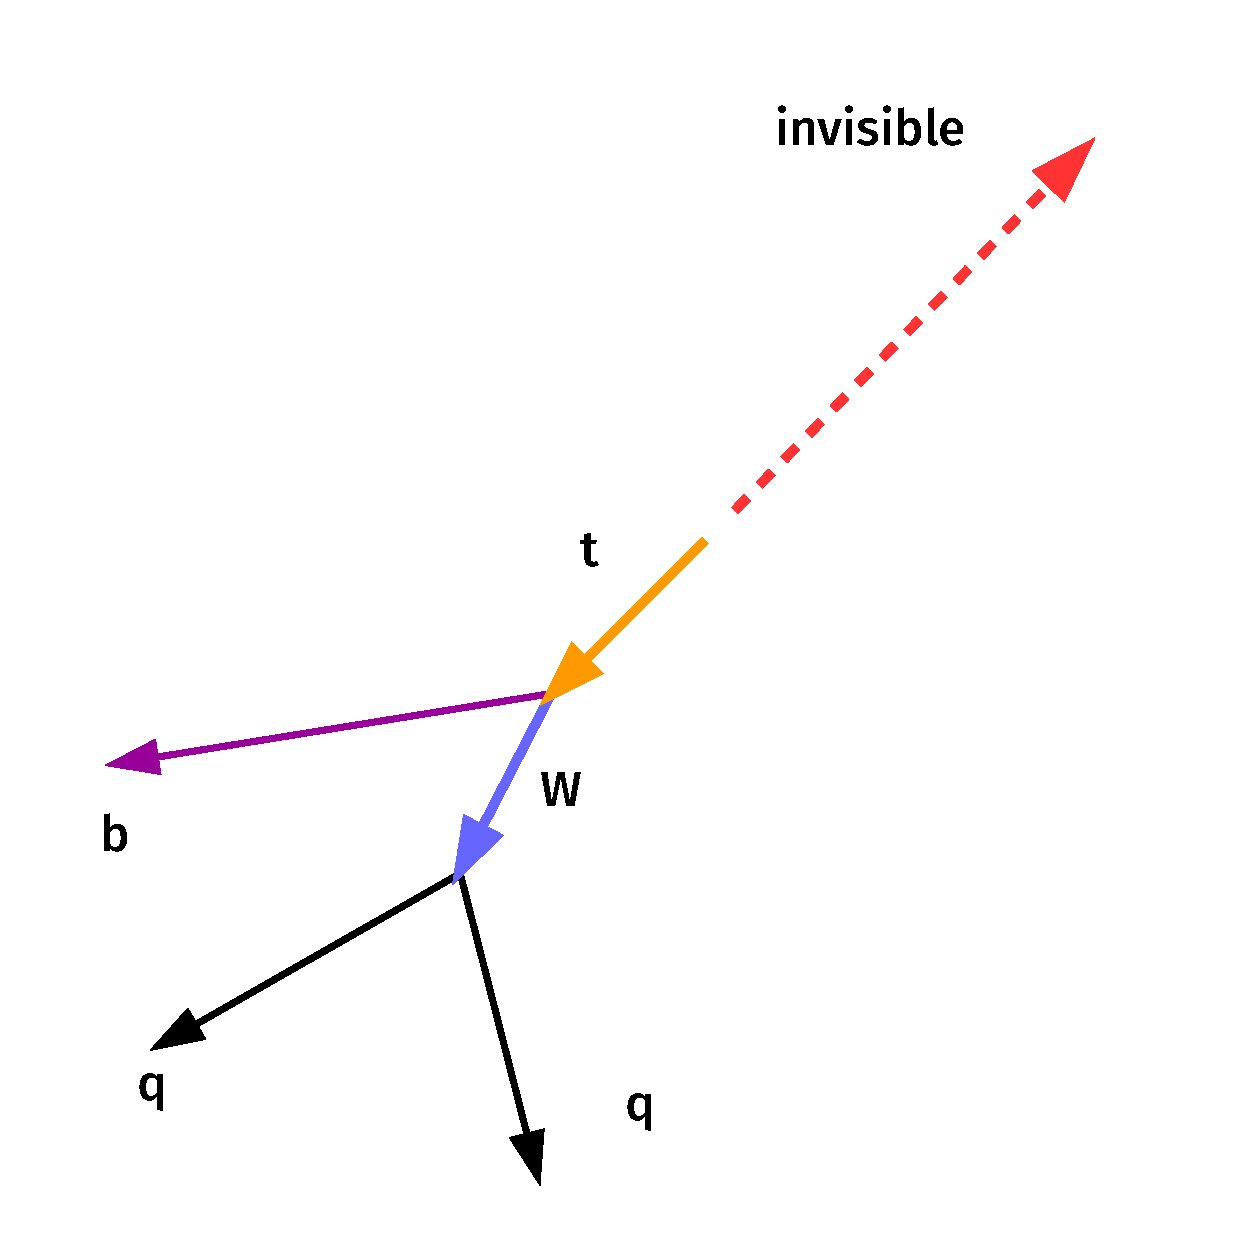
\includegraphics[width=\textwidth]{../figures/talk//parton_event.pdf}}
    \only<2-3>{Quarks shower and hadronize into jets \\
               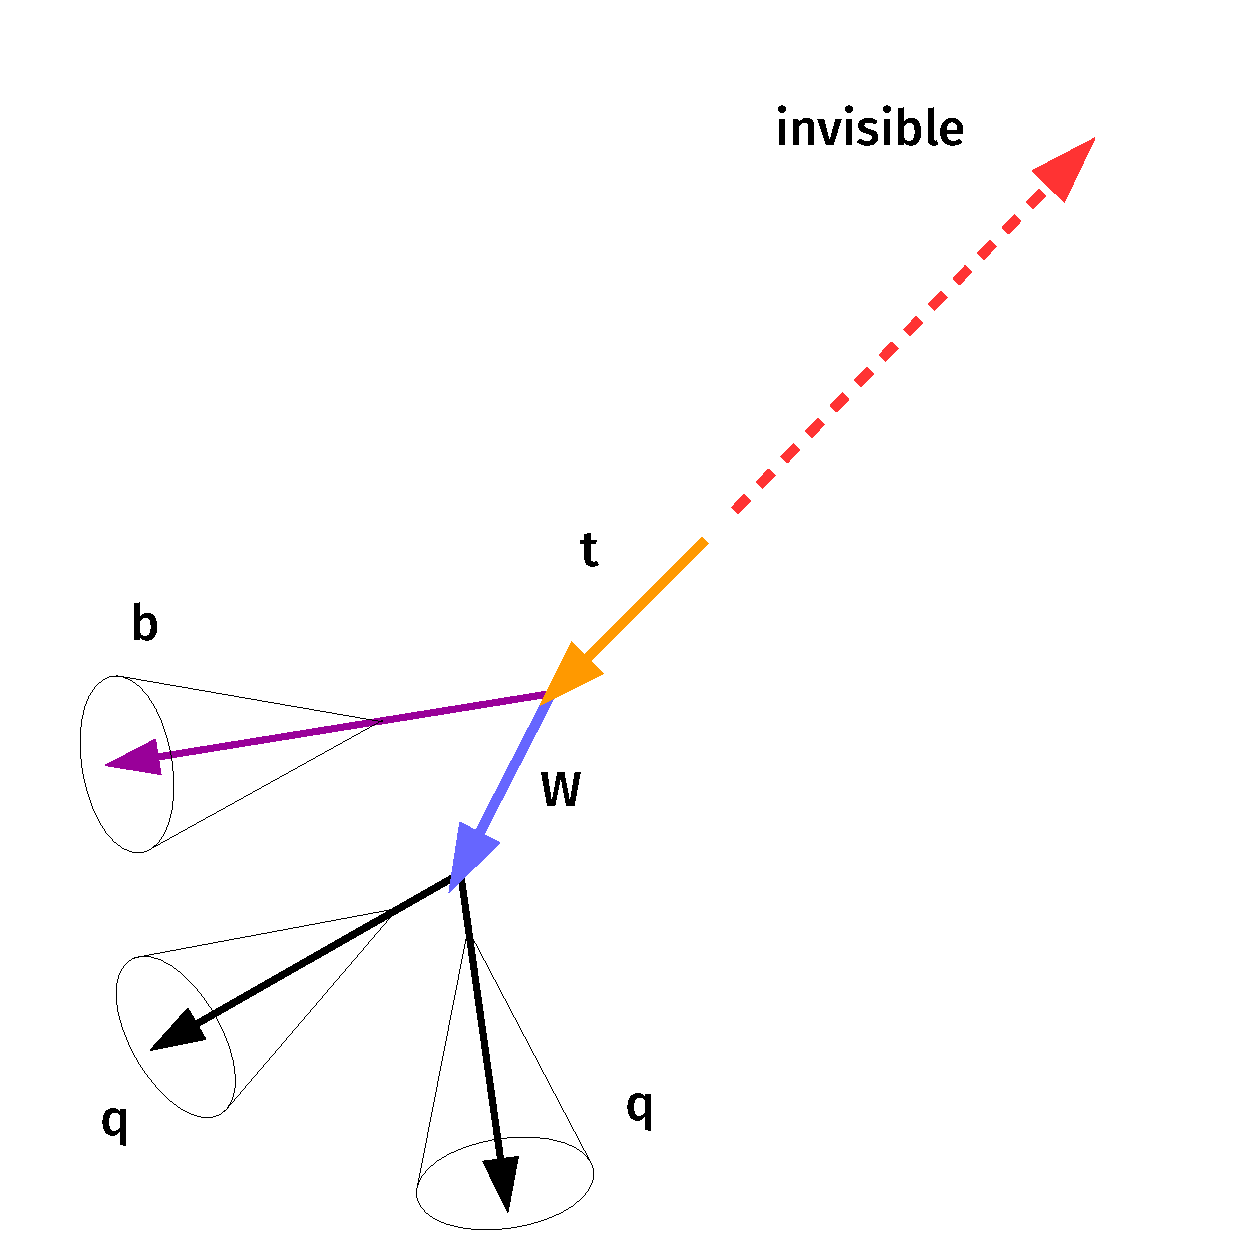
\includegraphics[width=\textwidth]{../figures/talk//resolved_event.pdf}}
    \only<4>{Decay products collimate
             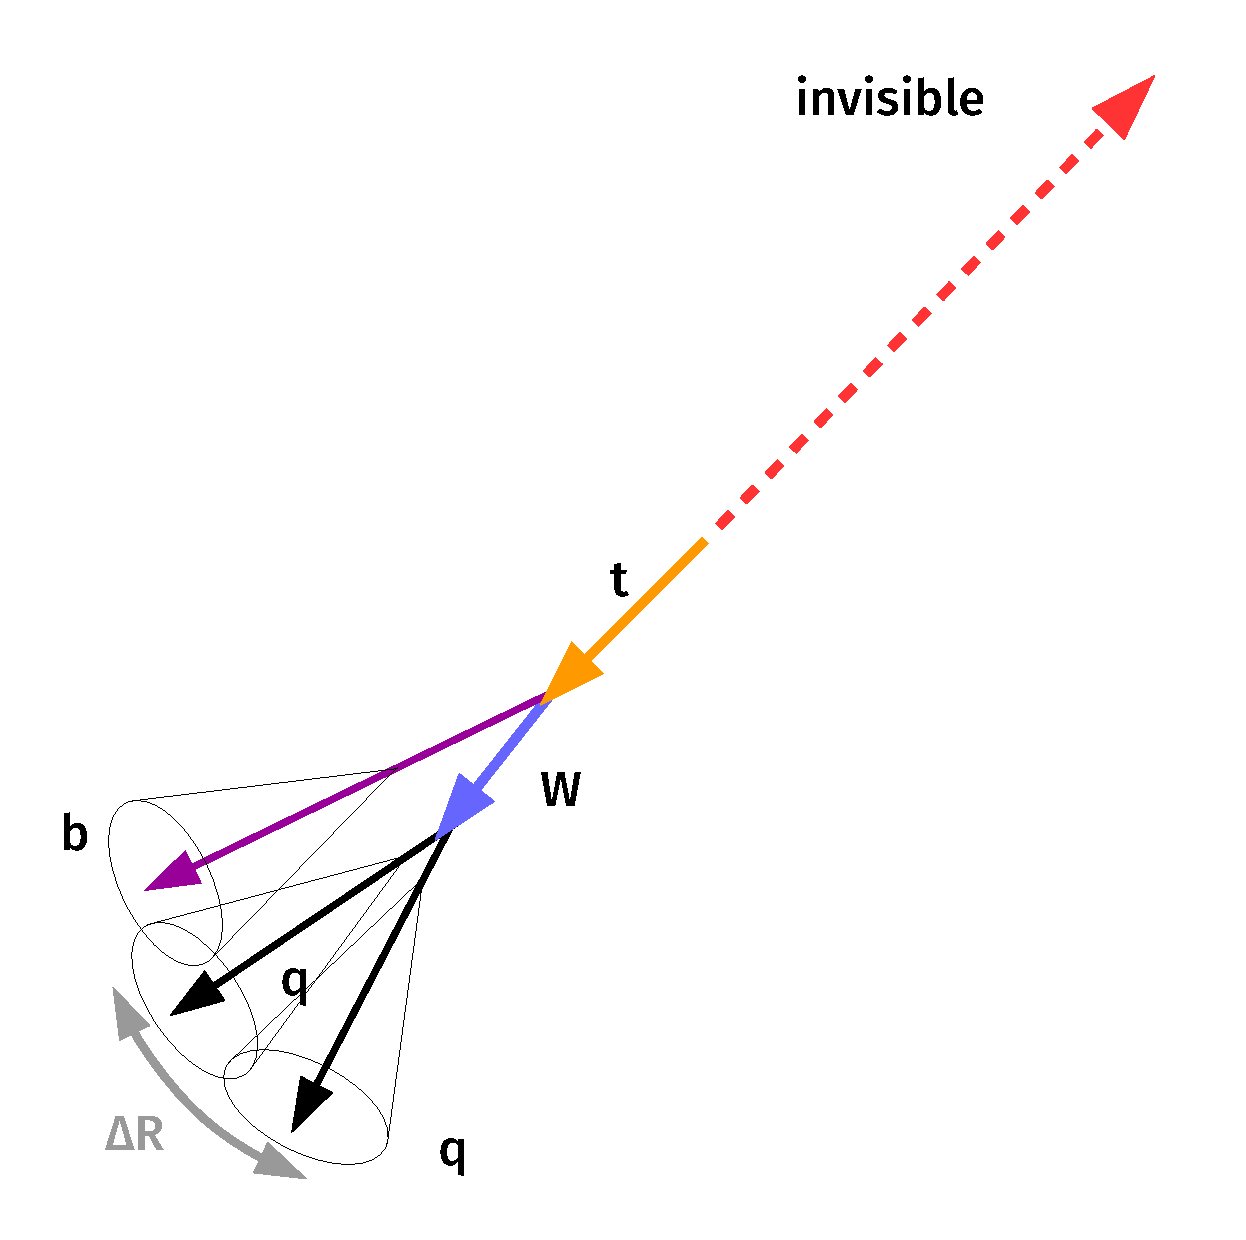
\includegraphics[width=\textwidth]{../figures/talk//boosted_event.pdf}}
  \end{column}
  \begin{column}{0.55\textwidth}
      \only<2>{
      \begin{itemize}
        \item Particles are clustered into jets based on a distance metric:
            \[d_{ij} = \min\{\pti^{2q}, \ptj^{2q}\} \frac{\Delta R(p_i^\mu, p_j^\mu)^2}{R}\]
        \item $q=-1$: anti-$k_\mathrm{T}$ (AK)
        \item $q=0$: Cambridge-Aachen (CA)
        \item Single-parton jet: AK $R=0.4$
      \end{itemize}
      \centering
        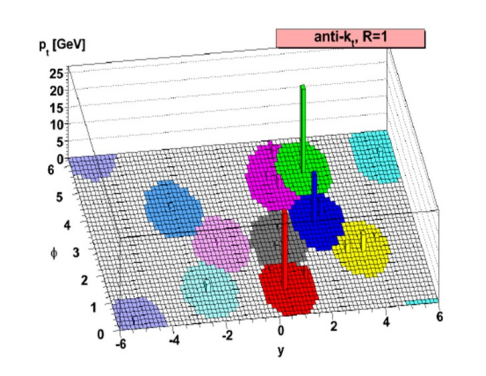
\includegraphics[width=0.4\textwidth]{../figures/talk/akt.png}
        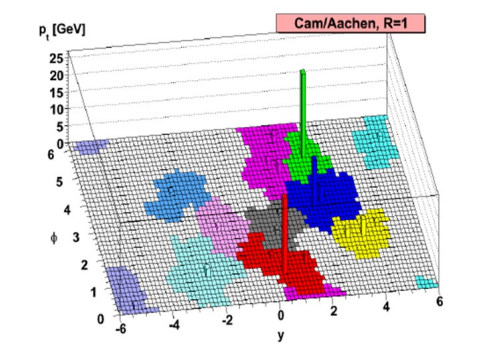
\includegraphics[width=0.4\textwidth]{../figures/talk/ca.png}
      }
      \uncover<3->{
      \vspace{-5mm}
            \begin{center}
              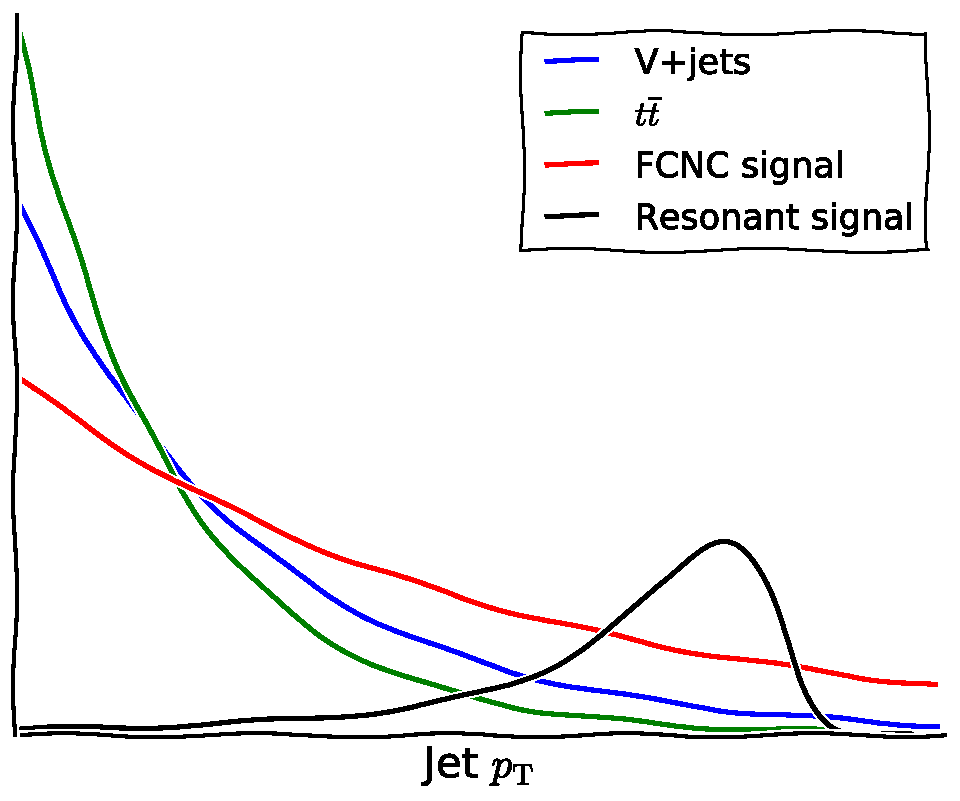
\includegraphics[width=0.6\textwidth]{../figures/talk/fatjetpt.pdf}
            \end{center}
      \vspace{-3mm}
        \begin{itemize}
            \item Signal more energetic than SM 
            \item Maximize S/B $\Rightarrow$ large jet $\pt$
      }
      \uncover<4->{
      \item Separation between jets: $\Delta R \sim 2 m_t /\pt $
      \begin{itemize}
        \item $\pt>250\,\gev$ $\Rightarrow$  jets ($R=0.4$) overlap
        \item $\Delta R = \sqrt{(\Delta\phi)^2 + (\Delta\eta)^2}$
      \end{itemize}
      }
      \uncover<3->{
      \end{itemize}
      }
  \end{column}
  \end{columns}
\end{frame}

\begin{frame}[t]   \frametitle{Reconstruction of top quark jet}
  \vspace{-5mm}
  \begin{columns}[T]
  \begin{column}{0.33\textwidth}
  \centering 
    Clustering 
    \begin{itemize}
      \item {\small Three AK $R=0.4$ jets $\rightarrow$ single CA $R=1.5$ jet}
    \end{itemize}
      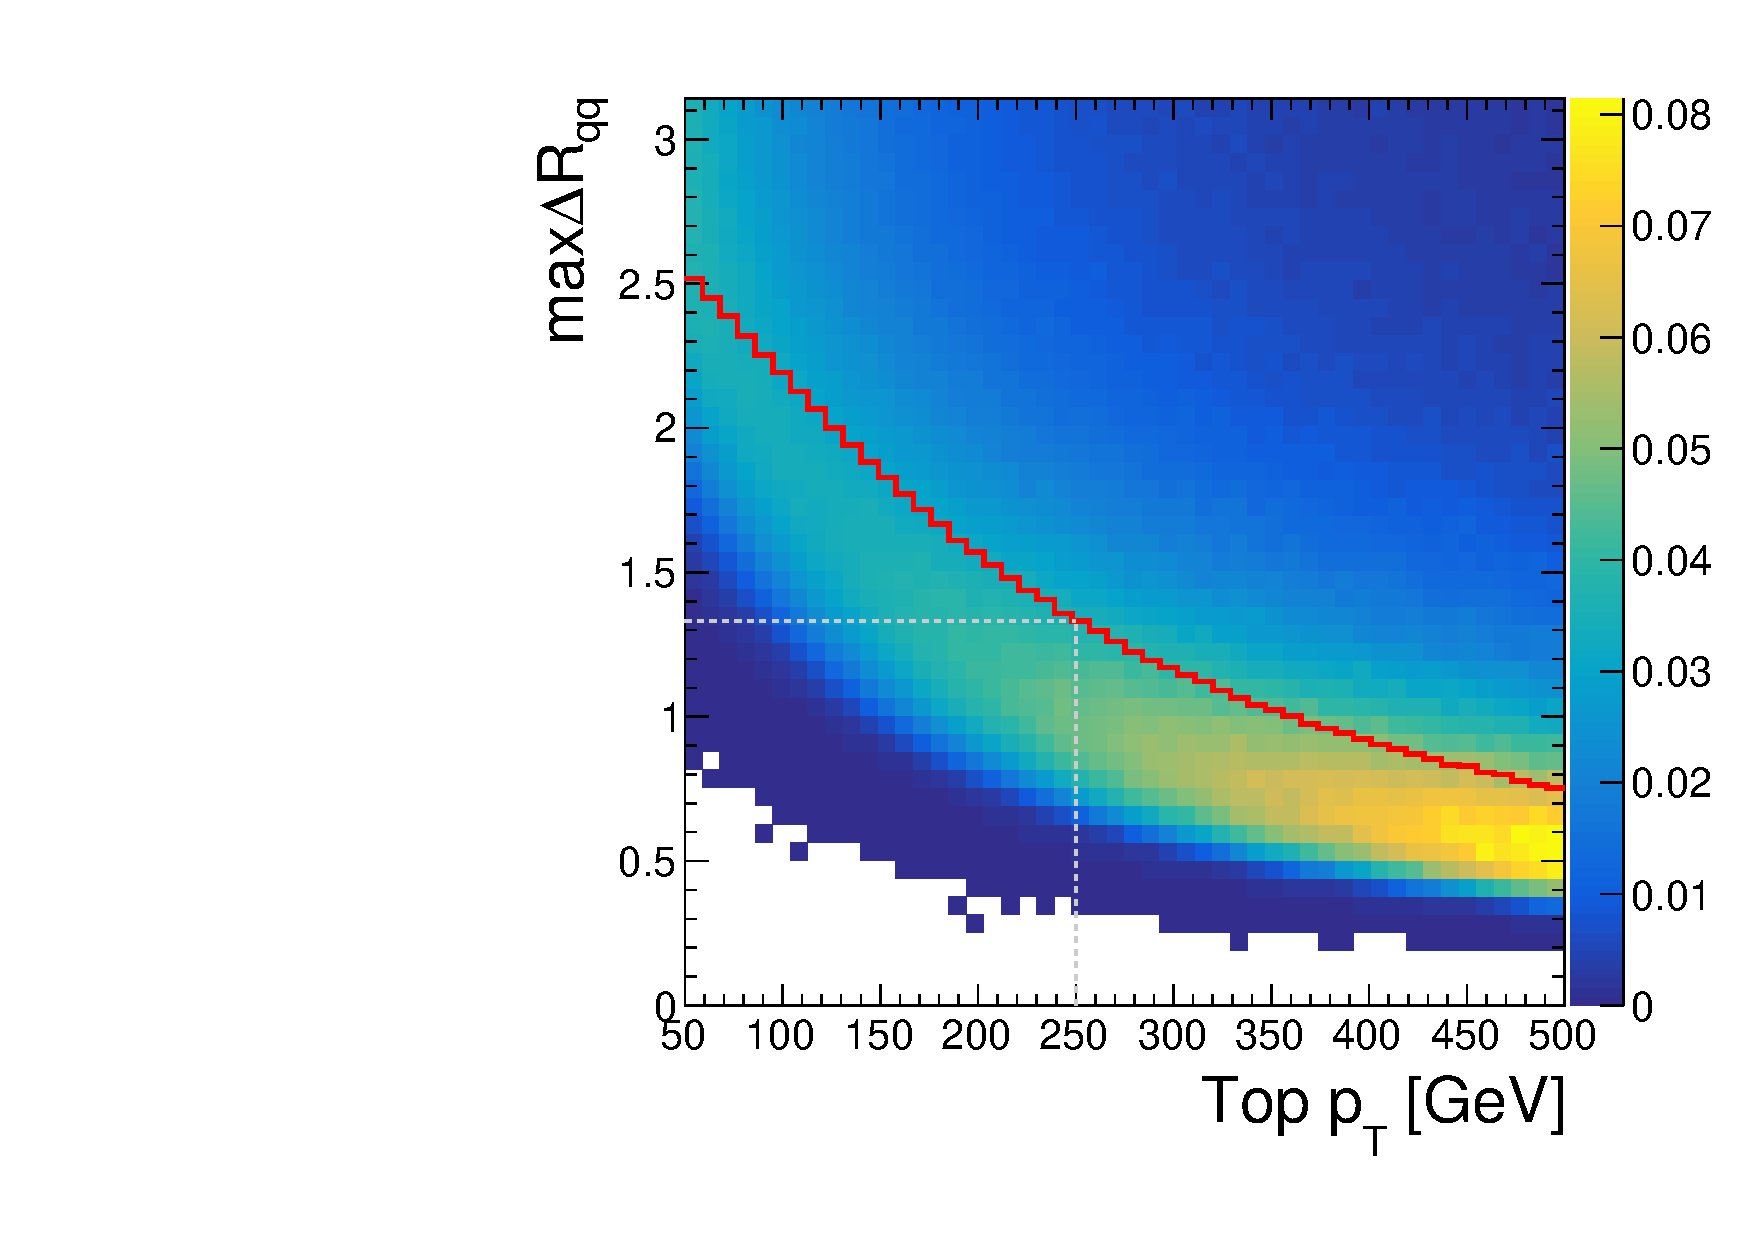
\includegraphics[width=0.8\textwidth]{../figures/toptagging/gen/ptdr.pdf}
      \vspace{-3mm}
    \begin{itemize}
      \item {\small These are huge jets: half the detector!}
      \item {\small Many extra particles}
    \end{itemize}
  \end{column}
  \pause 
  \begin{column}{0.33\textwidth}
  \centering 
    Pileup particles 
  \begin{itemize}
    \item {\small 10-25 vertices per collision}
    \item {\small PU particles are isotropic }
  \end{itemize}
      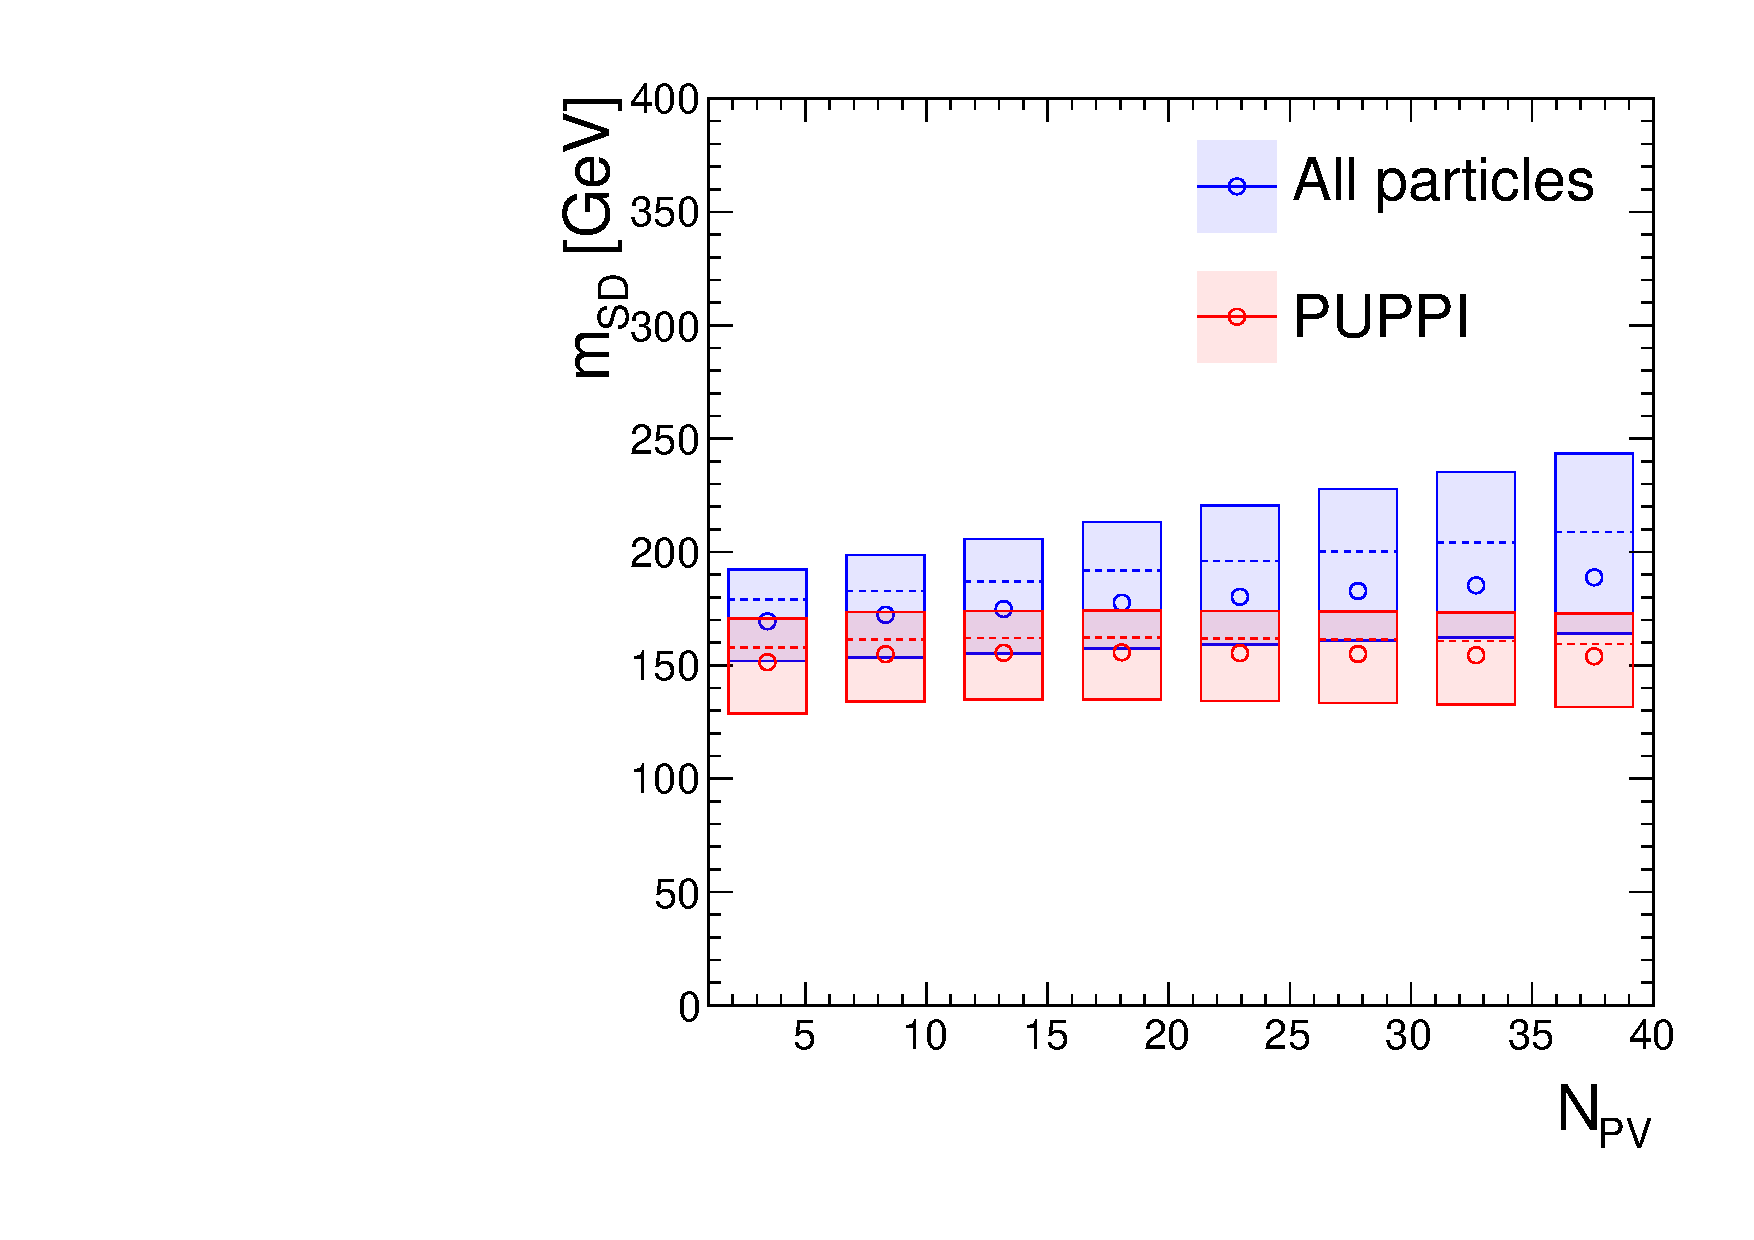
\includegraphics[width=0.8\textwidth]{../figures/toptagging/gen/npv_clf_MSD_ZpTT_lo.pdf}
      \vspace{-5mm}
  \begin{itemize}
    \item {\small \mlink{PUPPI} estimates $P(\mathrm{PU}|\pt,\eta,\phi)$ from proximity to PV particles}
  \end{itemize}
  \end{column}
  \pause 
  \begin{column}{0.33\textwidth}
    \centering 
    Non-PS radiation 
    \begin{itemize}
      \item {\small ISR, UE, MPI}
    \end{itemize}
      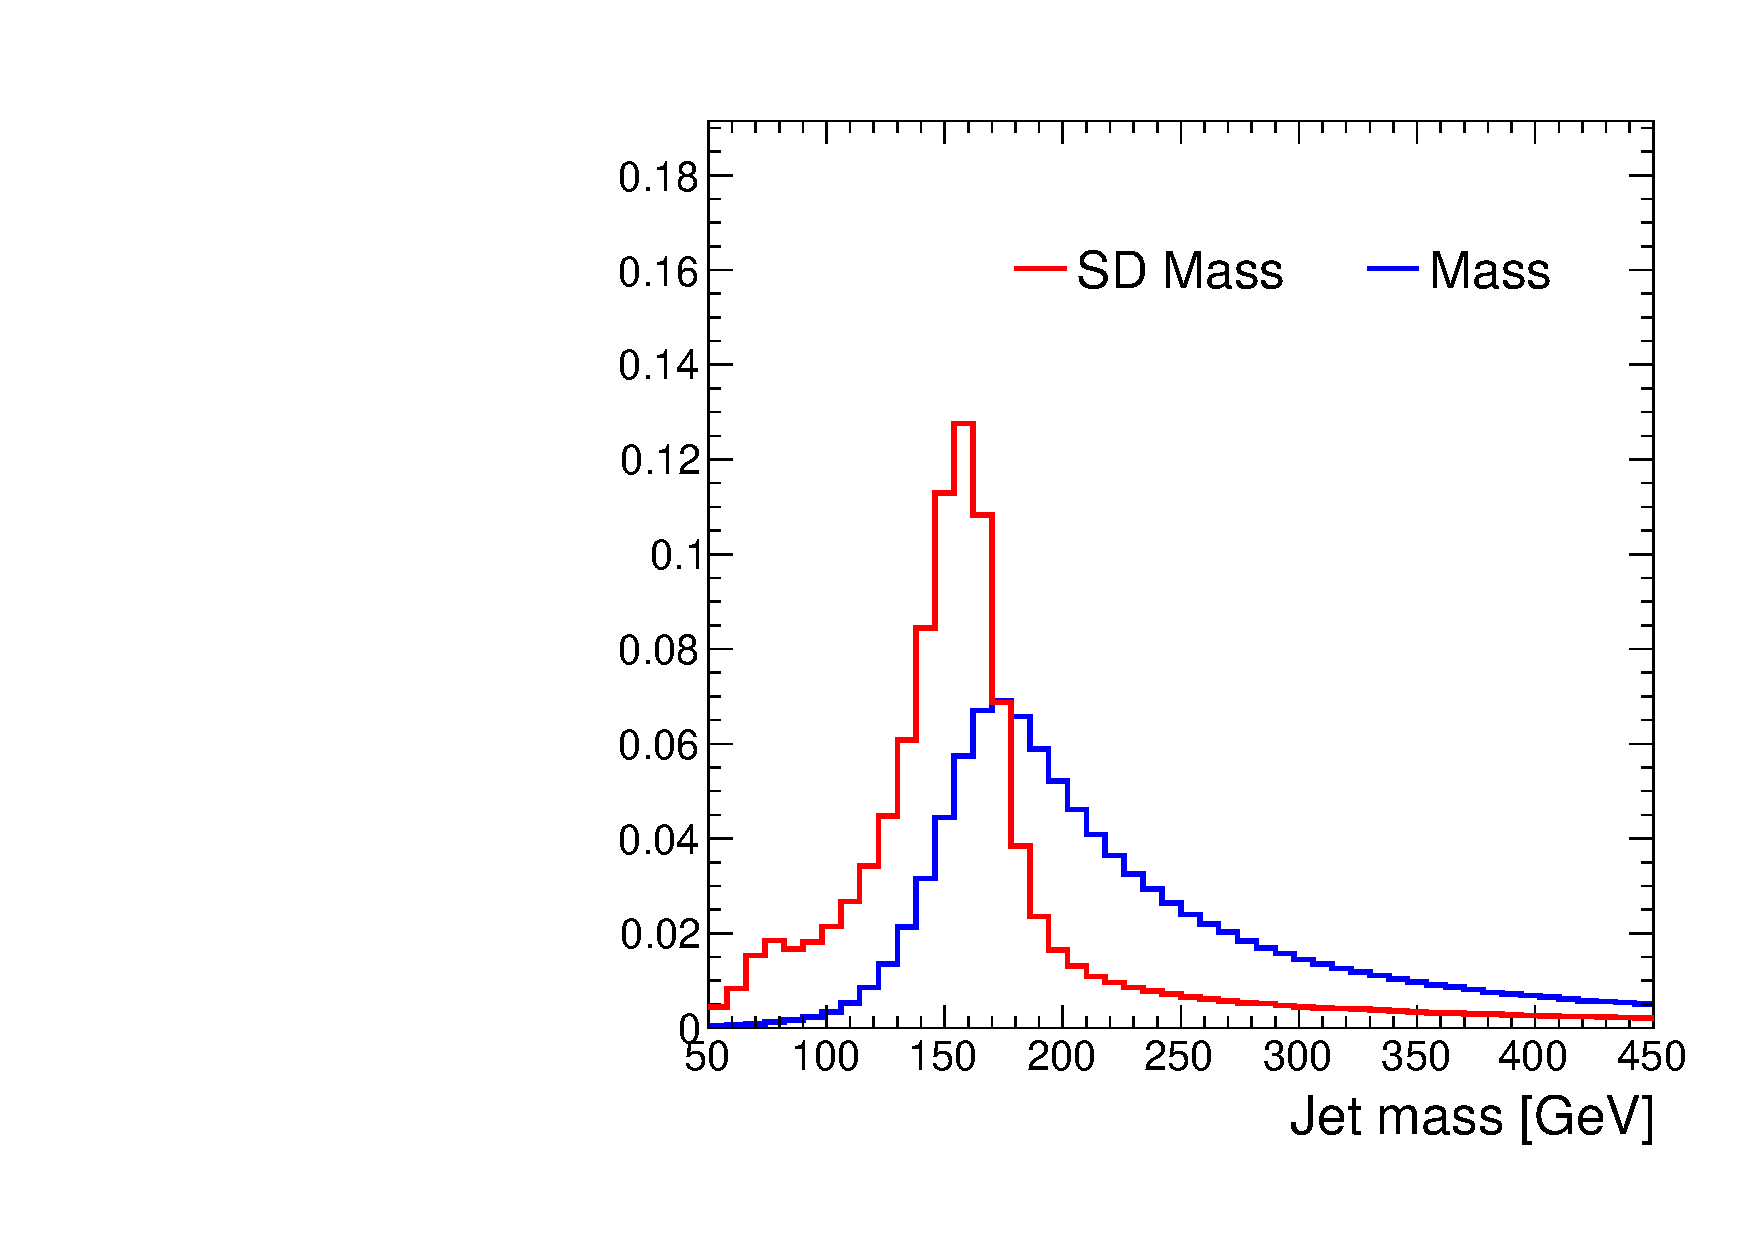
\includegraphics[width=0.8\textwidth]{../figures/toptagging/gen/compare_ZpTT_lo.pdf}
      \vspace{-3mm}
    \begin{itemize}
      \item {\small \mlink{Soft drop} removes wide-angle and soft radiation from jet}
    \end{itemize}
  \end{column}
  \end{columns}
\end{frame}

\begin{frame}[t]  \frametitle{Jet substructure}
  \begin{itemize}
    \item Top quark $\rightarrow$ 3q $\Rightarrow$ top jet has 3 ``prongs'': regions of correlated radiation
    \begin{center}
      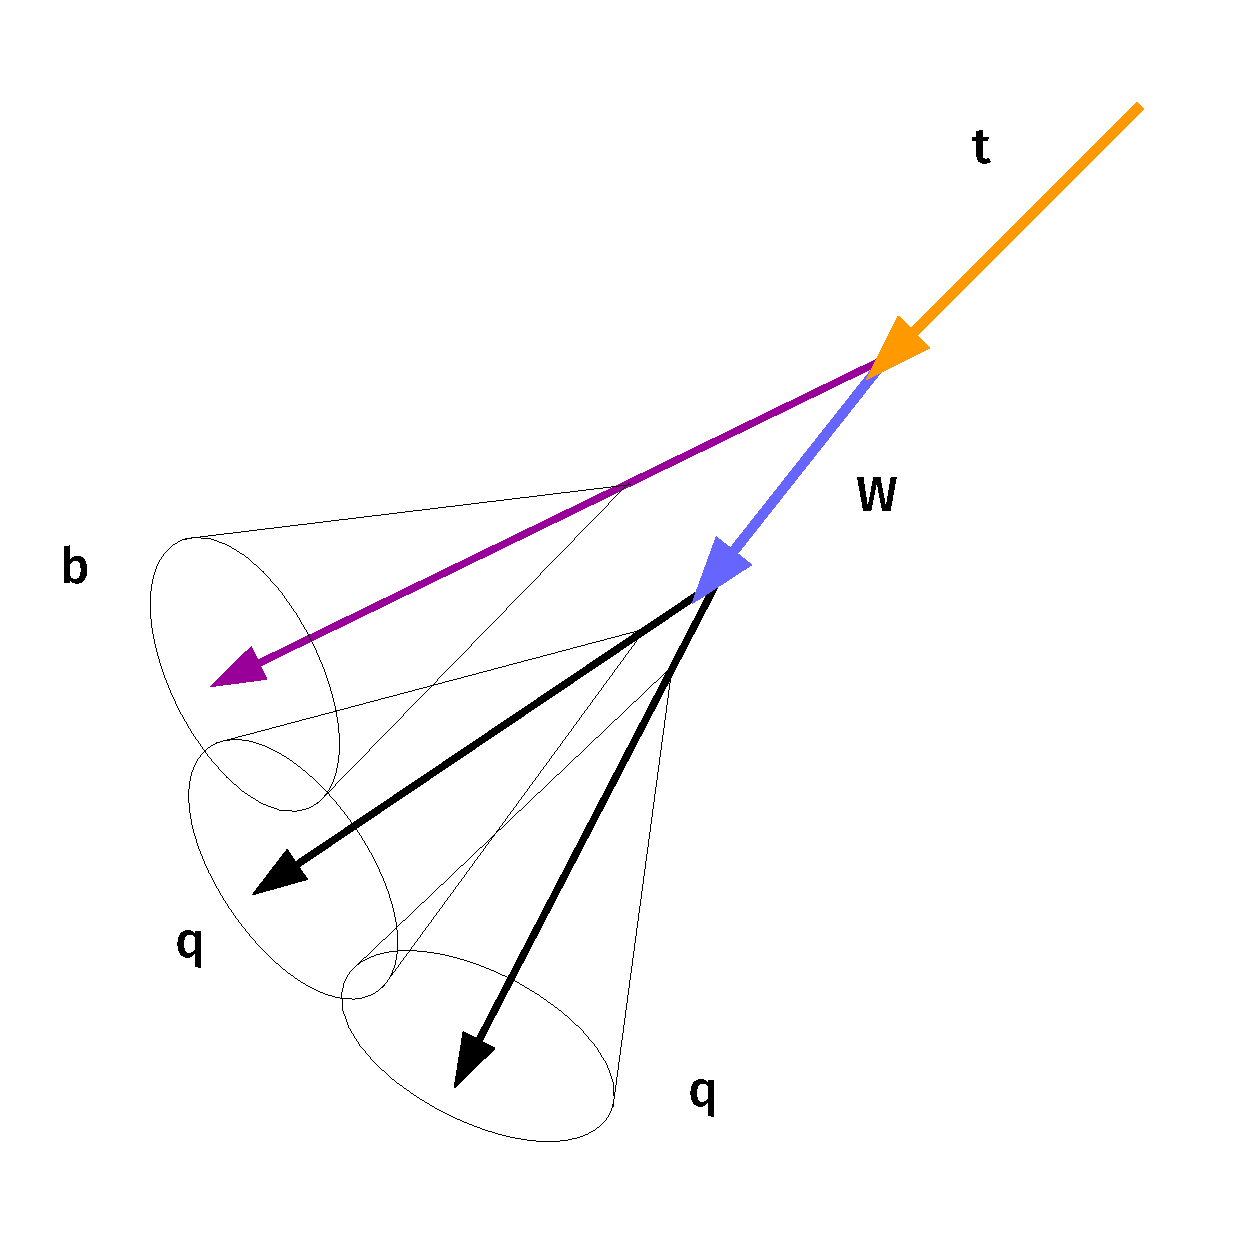
\includegraphics[width=0.3\textwidth]{../figures/talk/topjet.pdf} \hspace{10mm}
      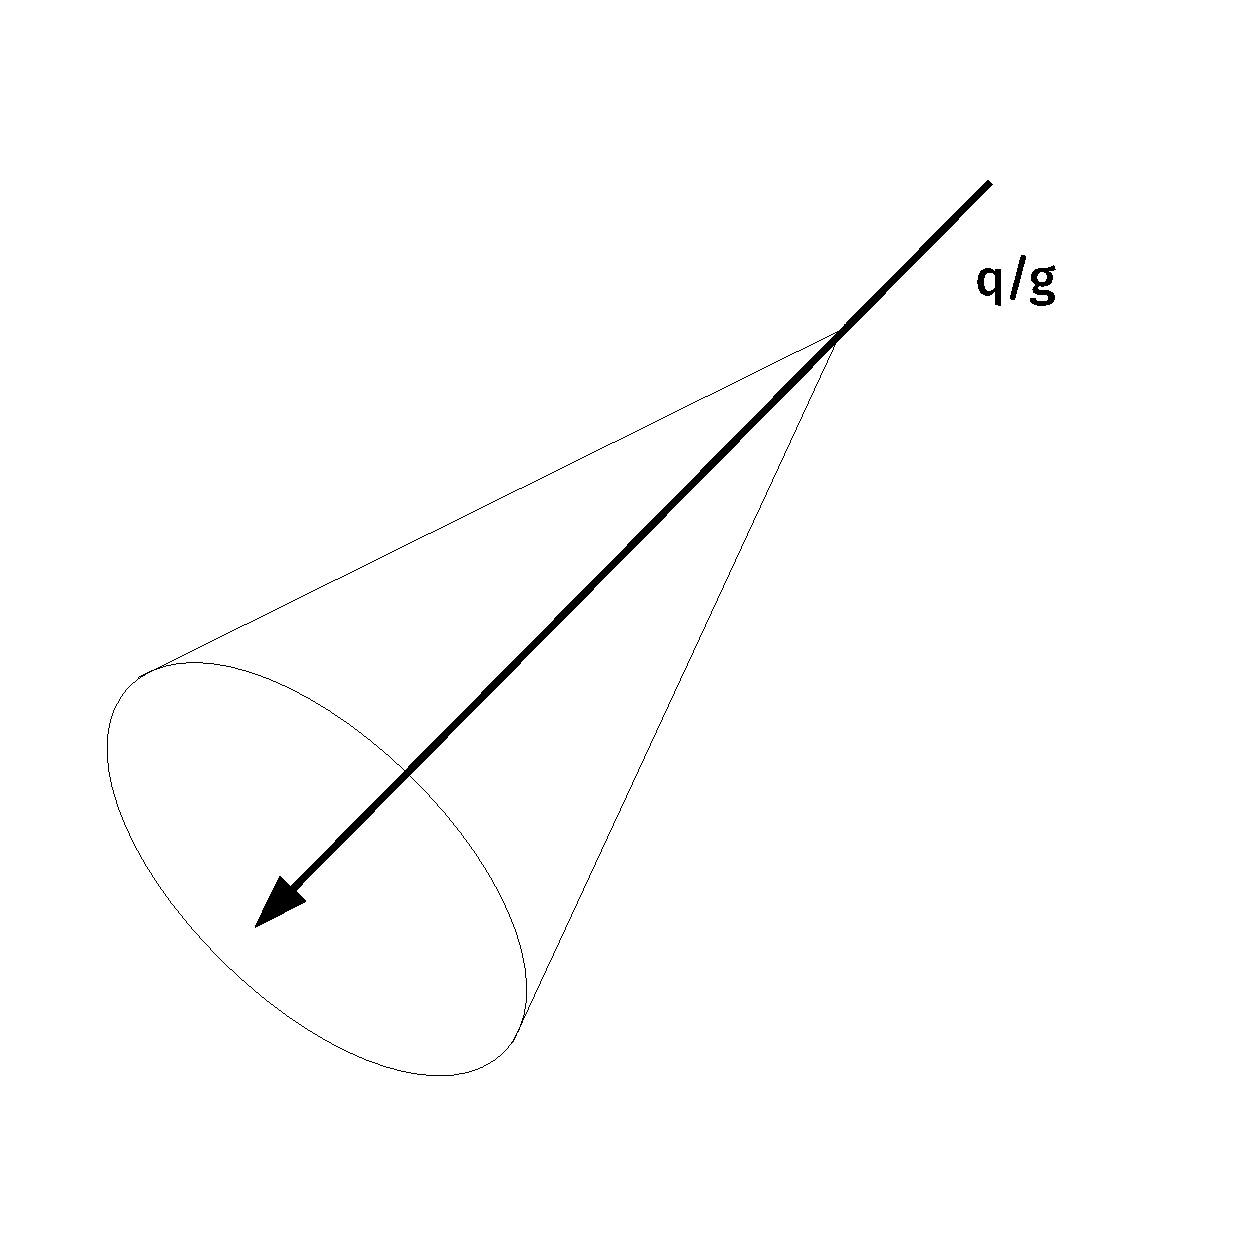
\includegraphics[width=0.3\textwidth]{../figures/talk/qgjet.pdf}
    \end{center}
    \item \mlink{Substructure} observables are sensitive to such features
    \begin{itemize}
      \item $N$-subjettiness, subjet algorithms, ECFs,\dots
    \end{itemize}
  \end{itemize}
\end{frame}

\begin{frame}[t]   \frametitle{Energy correlation functions}
  \vspace{-5mm}
  \centering
    ECFs are $\N$-point distance-weighted correlation functions among particles of the jet
    \vspace{3mm}
    \centering
    \begin{tabular}{ccccc}
      $e(a,\N,\alpha) \sim $ &
      $\displaystyle\sum _{\N \text{ particles }\in J}$ &
      $ \uncover<2->{\textcolor{mygrey}{ \left[\displaystyle\prod_{p\in \text{particles}} \dfrac{E_p}{{E_J}} \right]} $ &
      $\uncover<3->{\times} $ &
      $\uncover<3->{\textcolor{maroon}{\min\left\{\displaystyle\prod_{p,q \in \text{particles}}^a \theta(p,q) \right\}^\alpha}}} $ \\
      \\
      &
      sets of $\N$ particles &
      \uncover<2->{\textcolor{mygrey}{energy fractions}} &
      &
      \uncover<3->{\textcolor{maroon}{opening angle}}  \\
    \end{tabular}
    \begin{columns}
      \begin{column}{0.33\textwidth}
        \centering 
        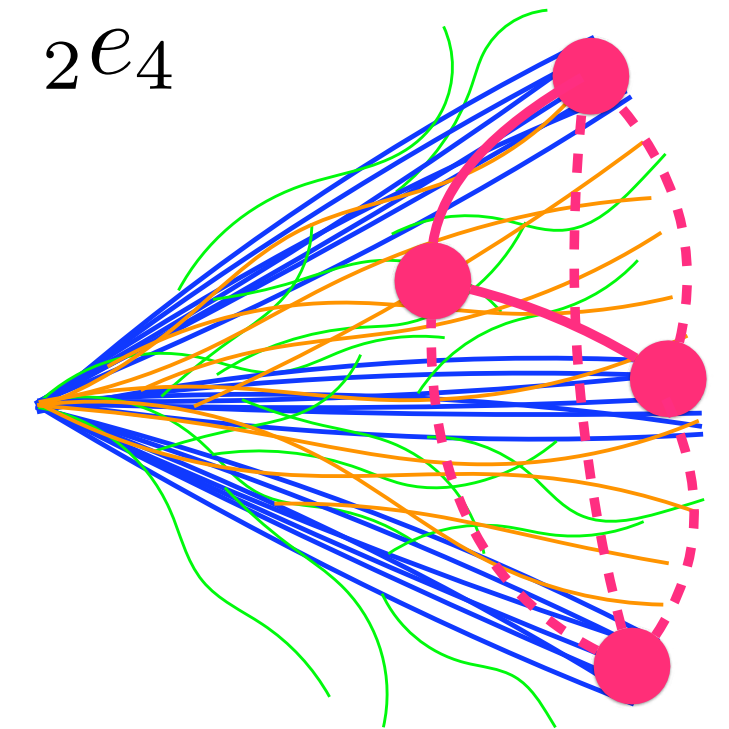
\includegraphics[width=0.67\textwidth]{../figures/talk/e4_3.png}\mycite{9}
      \end{column}
      \uncover<4->{
      \begin{column}{0.33\textwidth}
        \centering
        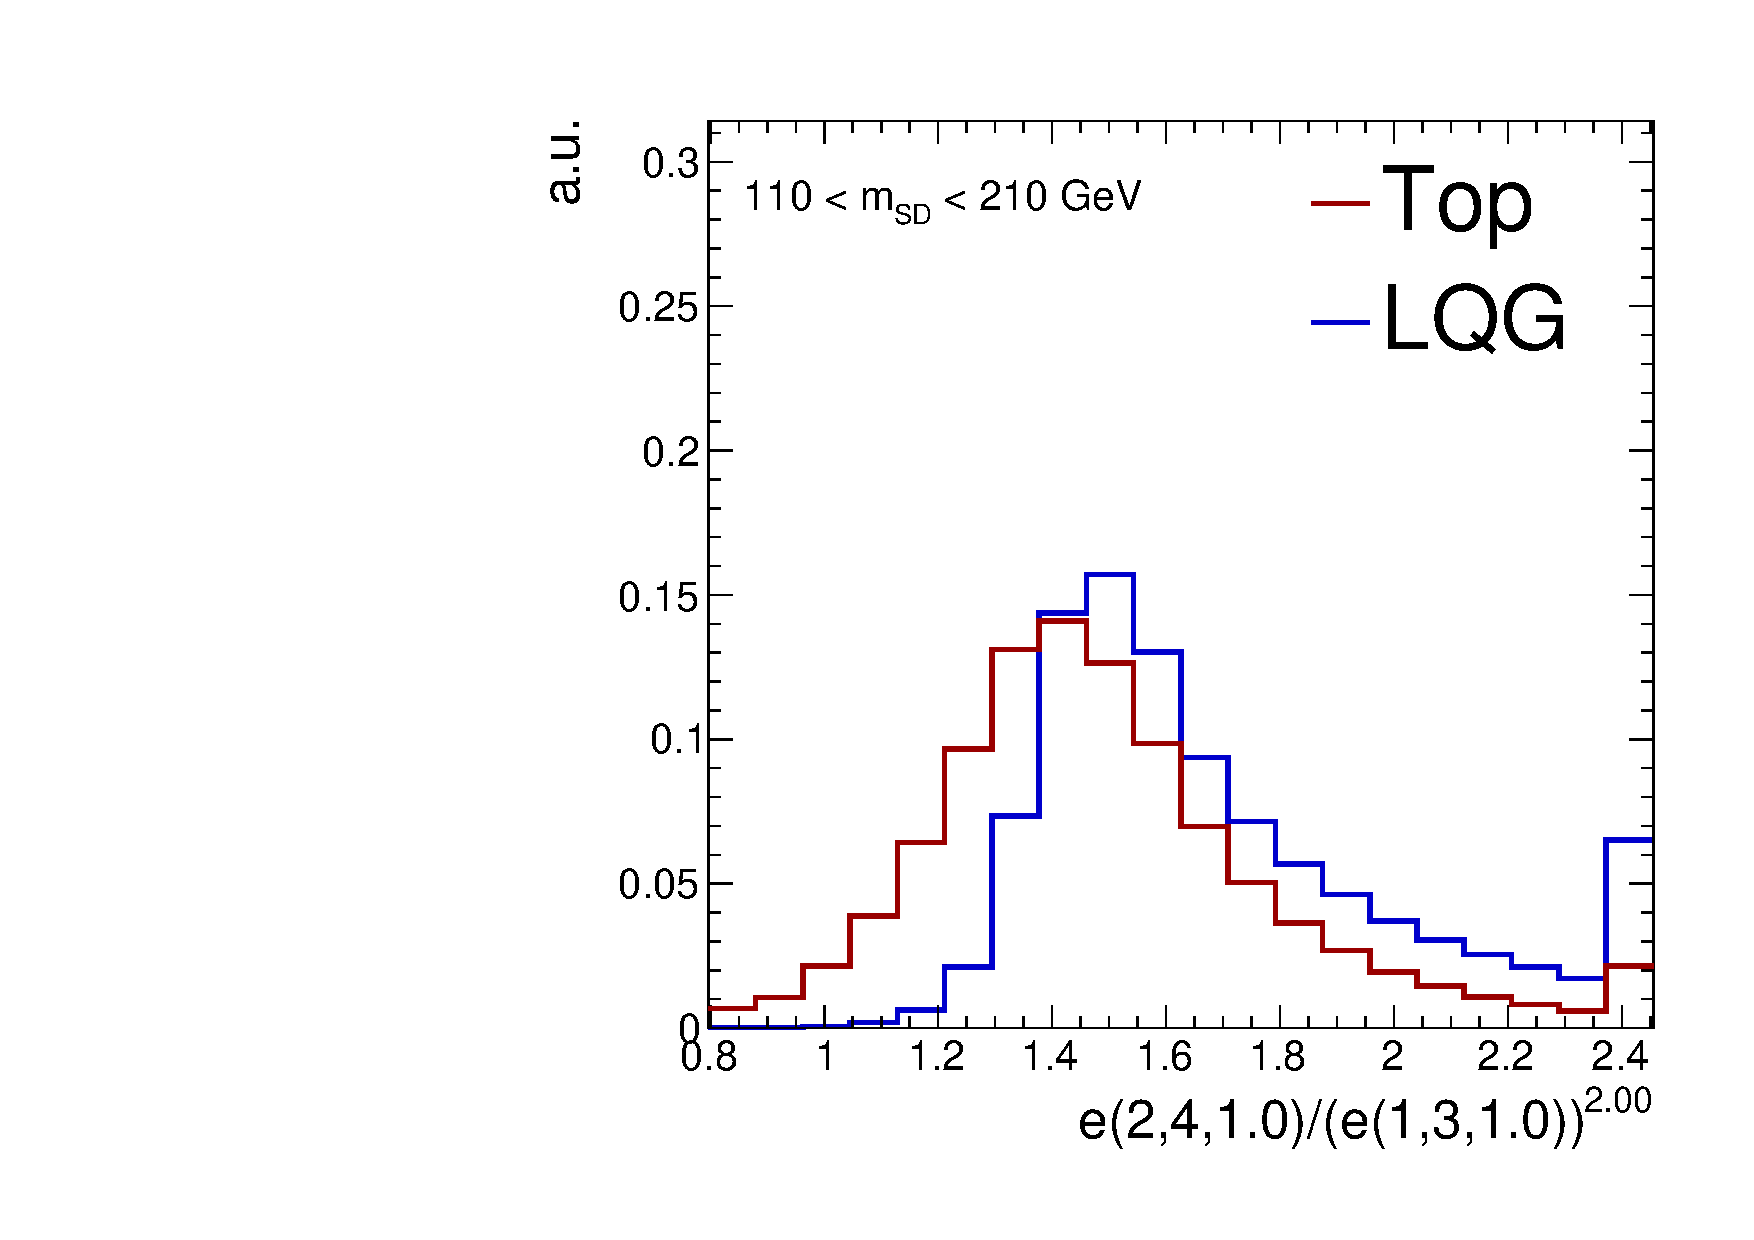
\includegraphics[width=0.67\textwidth]{../figures/toptagging/shapes/mass_ratio_24101310.pdf}
        \\ {\small $e(4)/e(3)$ }
      \end{column}
      }
      \uncover<5->{
      \begin{column}{0.33\textwidth}
        \centering 
        \includegraphics[width=0.67\textwidth]{../figures/toptagging/shapes/mass_ratio_12102205.pdf}
        \\ {\small $e(2)/e(2)$ }
      \end{column}
      }
      \end{columns}
\end{frame}

\begin{frame}[t] \frametitle{Building a combined tagger}
  \vspace{-5mm}
  \begin{columns}[T]
  \begin{column}{0.33\textwidth}
  \centering 
    Modeling issues 
    \vspace{-2mm}
    \[{\displaystyle \frac{e(a,N,\alpha)}{e(b,M,\beta)^x},~~ M \leq N, ~ x = \frac{a\alpha}{b\beta} }\] 
    \vspace{-4mm}
    \begin{itemize}
      \item {\small Some ECF ratios poorly described by PS model}
    \end{itemize}
        \only<1>{\includegraphics[width=0.8\textwidth]{../figures/toptagging/datamc/singlemuonw_ratio_22051240.pdf}}
        \only<2>{\includegraphics[width=0.8\textwidth]{../figures/toptagging/datamc/scanmnab.pdf}}
  \end{column}
  \begin{column}{0.33\textwidth}
  \centering 
    Dimensional reduction \\  
  \begin{itemize}
    \item {\small Large ECF ratio space}
    \item {\small Expensive to compute }
  \end{itemize}
      \includegraphics[width=0.8\textwidth]{../figures/toptagging/bdt/fakerate_vs_eff50.pdf}
      \vspace{-5mm}
  \begin{itemize}
    \item {\small Embed dimensional reduction into boosted decision tree training}
  \end{itemize}
  \end{column}
  \begin{column}{0.33\textwidth}
    \centering 
    Combined tagger \\ 
    \begin{itemize}
      \item {\small Final discriminator combines ECFs, $\tau_{32}$, $f_\mathrm{rec}$ }
    \end{itemize}
      \includegraphics[width=0.8\textwidth]{../figures/toptagging/bdt/roc.pdf}
      \vspace{-3mm}
    \begin{itemize}
      \item {\small 30\% better background rejection than $\tau_{32}$ }
    \end{itemize}
  \end{column}
  \end{columns}
\end{frame}

\begin{frame}[t]  \frametitle{Selecting mono-top events}
  \vspace{-5mm}
  \begin{columns}[T]
  \begin{column}{0.5\textwidth}
  \centering
    \includegraphics[width=0.8\textwidth]{../figures/talk/boosted_event.pdf}
  \end{column}
  \begin{column}{0.5\textwidth}
    \begin{itemize}
      \item $\ptmiss>250\,\gev$ (trigger)
      \item No $e,\mu,\tau_h$, and AK4 $b$ jets
      \item One CA15 jet, $\pt>250\,\gev$
      \begin{itemize}
        \item Selected by BDT \pause
        \item Mass consistent with $m_t$
        \item Signature of $B$ meson decay inside jet
        \begin{itemize}
          \item Lab frame $c\tau \sim \mathcal{O} (\mathrm{mm})$
        \end{itemize}
      \end{itemize}
    \end{itemize}
    \centering
    \vspace{-5mm}
    \hspace{-40mm}
      \includegraphics[width=0.45\textwidth]{../figures/toptagging/sf/tight_pass.pdf}
      \includegraphics[width=0.55\textwidth]{../figures/cms/csvv2.png}
  \end{column}
  \end{columns}
\end{frame}

\begin{frame}[t]  \frametitle{SM backgrounds}
  \centering
  \vspace{5mm}
  \begin{columns}
  \begin{column}{0.33\textwidth}
    \centering
    $Z\rightarrow\nu\nu $ ($30\%$) \\
    \includegraphics[width=\textwidth]{../figures/talk/zsr.pdf} \pause
  \end{column}
  \begin{column}{0.33\textwidth}
    \centering
    $W\rightarrow (\ell)\nu$ ($15\%$) \\
    \includegraphics[width=\textwidth]{../figures/talk/wsr.pdf} \pause
  \end{column}
  \begin{column}{0.33\textwidth}
    \centering
    $t$ quark pair ($50\%$) \\
    \includegraphics[width=\textwidth]{../figures/talk/ttsr.pdf} \pause
  \end{column}
  \end{columns}
  {\large
    Note that $\ptmiss$ is the transverse momentum of the \mlink{vector boson}
  }
\end{frame}

\begin{frame}[t]  \frametitle{Prediction of $Z$ $\ptmiss$ spectrum}
  \vspace{-5mm}
  \begin{itemize}
      \sitem{MC predictions have $\sim30\%$ uncertainties $\Rightarrow$ use data to constrain}
      \sitem{$\ptmiss$ is driven by jet measurement}
      \sitem{\mlink{Hadronic recoil} ($U$) $\equiv$ momentum imbalance if we pretend $\ell^\pm,\gamma$ are invisible. }
  \end{itemize}
  \begin{columns}
  \begin{column}{0.33\textwidth}
    \centering
    \includegraphics[width=\textwidth]{../figures/talk/zsr.pdf}\\ \vspace{-7mm}
    \textcolor{mygrey}{$Z\rightarrow\nu\nu$} (20.5\%) \\
  \end{column}
  \begin{column}{0.34\textwidth}
    \centering
    {\Large \textcolor{mygrey}{$\ptmiss$} $\longleftrightarrow$ \textcolor{maroon}{$ \ptmiss$(no $\ell$)}} \\
    \vspace{5mm}
    In both cases: \\
    {\Large $U \approx \pt^Z$}
  \end{column}
  \begin{column}{0.33\textwidth}
    \centering
    \includegraphics[width=\textwidth]{../figures/talk/zcr.pdf} \\ \vspace{-7mm}
    \textcolor{maroon}{$Z\rightarrow\ell\ell$} (6.8\%) \\
  \end{column}
  \end{columns}
\end{frame}

\begin{frame} \frametitle{The real observable: $T = Z(\rightarrow\nu\nu)/Z(\rightarrow \ell\ell)$}
  \vspace{-5mm}
  \begin{columns}
    \begin{column}{0.3\textwidth}
      \includegraphics[width=\textwidth]{../figures/monotop/postfit/stackedPostfit_signal_monotop.pdf}
    \end{column}
    \begin{column}{0.05\textwidth} $\Big/$ \end{column}
    \begin{column}{0.3\textwidth}
      \includegraphics[width=\textwidth]{../figures/monotop/postfit/stackedPostfit_dielectron_monotop.pdf}
    \end{column}
    \begin{column}{0.05\textwidth} $=$  \end{column}
    \begin{column}{0.3\textwidth}
      \includegraphics[width=\textwidth]{../figures/monotop/xfer/rfactor_dielectron.pdf}
    \end{column}
  \end{columns}
  \begin{columns}[T]
    \begin{column}{0.7\textwidth}
      \begin{itemize}
        \item Exp. and MC stat. uncertainties are small ($\leq 7\%$)
        \item Jet-related experimental uncertainties cancel 
        \item Data stat. uncertainties are large at high $U$
        \pause 
        \item Compare to LO-to-NLO effect (+40\% to -30\%)
      \end{itemize}
    \end{column}
    \begin{column}{0.3\textwidth}
      \vspace{-6.5mm}
      \includegraphics[width=0.8\textwidth]{../figures/monotop/kfactors/zcorr_ptv.pdf}
    \end{column}
  \end{columns}
\end{frame}
 
\begin{frame} \frametitle{Additional constraints: $Z/\gamma$, $Z/W$}
  \vspace{-5mm}
  \begin{columns}
    \begin{column}{0.3\textwidth}
      \only<1>{\includegraphics[width=\textwidth]{../figures/talk/zsr.pdf}}
      \only<2>{\includegraphics[width=\textwidth]{../figures/monotop/postfit/stackedPostfit_signal_monotop.pdf}}
    \end{column}
    \begin{column}{0.05\textwidth} \only<2>{$\Big/$} \end{column}
    \begin{column}{0.3\textwidth}
      \only<1>{\includegraphics[width=\textwidth]{../figures/talk/wcr.pdf}}
      \only<2>{\includegraphics[width=\textwidth]{../figures/monotop/postfit/stackedPostfit_photon_monotop.pdf}}
    \end{column}
    \begin{column}{0.05\textwidth} \only<2>{$=$}  \end{column}
    \begin{column}{0.3\textwidth}
      \only<1>{\includegraphics[width=\textwidth]{../figures/talk/acr.pdf}}
      \only<2>{\includegraphics[width=\textwidth]{../figures/monotop/xfer/rfactor_photon.pdf}}
    \end{column}
  \end{columns}
  \begin{columns}[T]
    \begin{column}{0.7\textwidth}
      \begin{itemize}
        \item Higher-order corrections needed for $Z/\gamma$ and $Z/W$ predictions 
        \item Total (partial) cancellation of jet (theory) uncertainties
        \only<2>{\item Small data stat. uncertainties}
      \end{itemize}
    \end{column}
    \begin{column}{0.3\textwidth}
      \vspace{-6.5mm}
      \only<2>{\includegraphics[width=0.8\textwidth]{../figures/monotop/xfer/rfactor_wz.pdf}}
    \end{column}
  \end{columns}
\end{frame}

\begin{frame} \frametitle{Extrapolation uncertainties}
  \vspace{-5mm}
  \begin{columns}
    \begin{column}{0.5\textwidth}
      \centering
      \only<1>{
      $Z(\nu\nu)/Z(\mu\mu)$ \\
      \includegraphics[width=0.8\textwidth]{../figures/monotop/uncertainties/variations_dimuon.pdf} \\
      }
      \only<2>{
      $Z(\mu\mu)/Z(ee)$ \\
      \includegraphics[width=0.7\textwidth]{../figures/monotop/ratios/ratio_loose_zmm_zee_shapes_fit_b.pdf} \\
      }
      Small experimental uncertainties
    \end{column}
    \begin{column}{0.5\textwidth}
      \centering
      \only<1>{
      $Z(\nu\nu)/\gamma$ \\
      \includegraphics[width=0.8\textwidth]{../figures/monotop/uncertainties/variations_photon.pdf} \\
      }
      \only<2>{
      $Z(\mu\mu)/\gamma$ \\
      \includegraphics[width=0.7\textwidth]{../figures/monotop/ratios/ratio_loose_pho_zmm_shapes_fit_b.pdf} \\
      }
      Large theoretical uncertainties
    \end{column}
  \end{columns}
\end{frame}

\begin{frame}[t]  \frametitle{Background estimation summary}
  \begin{minipage}{\textwidth}
  \centering
  \begin{tikzpicture}[<->,>=stealth',shorten >=1pt,auto,node distance=3cm,
                    semithick,text width=1.5cm,align=center]
    % \tikzstyle{every state}=[fill=red,draw=none,text=white]

    \node[state,color=red] (ZvvSR)                    {\textcolor{black}{$Z\rightarrow\nu\nu$\\SR}};
    \node[state,color=blue] (ZllCR) [above left of=ZvvSR] {\textcolor{black}{$Z\rightarrow\ell\ell$\\ $\ell\ell$ CR}};
    \node(ZllDiag) [right of=ZllCR] {\hspace{-12mm}\includegraphics[width=1.5\textwidth]{../figures/talk/zcr.pdf}};

    \path[dashed]
          (ZvvSR) edge          node {} (ZllCR)
    ;
  \end{tikzpicture}
  \end{minipage}
\end{frame}

\begin{frame}[t]   \frametitle{Background estimation summary}
  \begin{minipage}{\textwidth}
  \centering
  \begin{tikzpicture}[<->,>=stealth',shorten >=1pt,auto,node distance=3cm,
                    semithick,text width=1.5cm,align=center]
    % \tikzstyle{every state}=[fill=red,draw=none,text=white]

    \node[state,color=red] (ZvvSR)                    {\textcolor{black}{$Z\rightarrow\nu\nu$\\SR}};
    \node[state,color=blue] (ZllCR) [above left of=ZvvSR] {\textcolor{black}{$Z\rightarrow\ell\ell$\\ $\ell\ell$ CR}};
    \node[state,color=black!60!blue] (ACR) [below left of=ZvvSR] {\textcolor{black}{$\gamma$\\$\gamma$ CR}};
    \node[state,color=red]         (WlvSR) [right of=ZvvSR]   {\textcolor{black}{$W\rightarrow\ell\nu$\\SR}};
    \node(ZllDiag) [right of=ZllCR] {\hspace{-12mm}\includegraphics[width=1.5\textwidth]{../figures/talk/zcr.pdf}};
    \node(ADiag) [right of=ACR] {\hspace{-12mm}\includegraphics[width=1.5\textwidth]{../figures/talk/acr.pdf}};

    \path[dashed]
          (ZvvSR) edge          node {} (ZllCR)
    ;
    \path
          (ZvvSR) edge          node {} (ACR)
          (ZvvSR) edge          node {} (WlvSR)
    ;
  \end{tikzpicture}
  \end{minipage}
\end{frame}

\begin{frame}[t]   \frametitle{Background estimation summary}
  \begin{minipage}{\textwidth}
  \centering
  \begin{tikzpicture}[<->,>=stealth',shorten >=1pt,auto,node distance=3cm,
                    semithick,text width=1.5cm,align=center]
    % \tikzstyle{every state}=[fill=red,draw=none,text=white]

    \node[state,color=red] (ZvvSR)                    {\textcolor{black}{$Z\rightarrow\nu\nu$\\SR}};
    \node[state,color=blue] (ZllCR) [above left of=ZvvSR] {\textcolor{black}{$Z\rightarrow\ell\ell$\\ $\ell\ell$ CR}};
    \node[state,color=black!60!blue] (ACR) [below left of=ZvvSR] {\textcolor{black}{$\gamma$\\$\gamma$ CR}};
    \node[state,color=red]         (WlvSR) [right of=ZvvSR]   {\textcolor{black}{$W\rightarrow\ell\nu$\\SR}};
    \node[state,color=orange] (WlvCR) [above right of=WlvSR]  {\textcolor{black}{$W\rightarrow\ell\nu$\\$\ell$ CR}};
    \node[state,color=red] (ttSR) [below right of=WlvCR] {\textcolor{black}{$t\bar{t}$\\SR}};
    \node[state,color=orange] (ttWCR) [above right of=ttSR]  {\textcolor{black}{$t\bar{t}$\\$\ell$ CR}};
    \node[state,color=black!60!green] (tttCR) [below right of=ttSR]  {\textcolor{black}{$t\bar{t}$\\$b\ell$ CR}};
    \node(ZllDiag) [right of=ZllCR] {\hspace{-12mm}\includegraphics[width=1.5\textwidth]{../figures/talk/zcr.pdf}};
    \node(WlvDiag) [left of=WlvCR] {\includegraphics[width=1.5\textwidth]{../figures/talk/wcr.pdf}\hspace{-40mm}};
    \node(ADiag) [right of=ACR] {\hspace{-12mm}\includegraphics[width=1.5\textwidth]{../figures/talk/acr.pdf}};
    \node(ttDiag) [right of=ttSR] {\includegraphics[width=1.5\textwidth]{../figures/talk/ttcr.pdf}};

    \path[dashed]
          (ZvvSR) edge          node {} (ZllCR)
          (WlvSR) edge          node {} (WlvCR)
          (ttSR)  edge          node {} (tttCR)
          (ttSR)  edge          node {} (ttWCR)
    ;
    \path
          (ZvvSR) edge          node {} (ACR)
          (ZvvSR) edge          node {} (WlvSR)
    ;
  \end{tikzpicture}
  \end{minipage}
  \put(-270,-45){Largest uncertainties:}
  \put(-270,-60){- $\ell$, $b$ ID; trigger }
  \put(-270,-75){- $\gamma/Z$ and $W/Z$ prediction}
\end{frame}

\begin{frame}[t] \frametitle{Likelihood maximization}
  
  \centering 
  Likelihood assuming one major background $(Z\rightarrow\nu\nu)$ and one CR :

  \begin{align*}
    \mathcal{L}(\bm{d} ~|~ \mu, \bm\mu^Z, \bm\theta) =~& \prod_{i} \mathrm{Pois}\left(d_i^\mathrm{SR} ~|~ \mu S_i(\bm\theta) + \mu^Z_i + B_i^\mathrm{SR}(\bm\theta)\right) \\
                                                      &\times \prod_{i}\mathrm{Pois}\left(d_i^\mathrm{CR} ~\Big|~ \frac{\mu^Z_i}{T_i(\bm\theta)} + B_i^\mathrm{CR}(\bm\theta)\right) \\ 
                                                      &\times \prod_j p(\theta_j)
  \end{align*}
\end{frame}


\begin{frame}[t] \frametitle{MLE recoil distributions (SM hypothesis)}
  \vspace{-7mm}
  \begin{columns}[T]
    \begin{column}{0.25\textwidth}
      \centering
      \vspace{-3.5mm}
      \includegraphics[width=\textwidth]{../figures/monotop/postfit/stackedPostfit_signal_monotop.pdf}\\
      \vspace{-5.5mm}
      \includegraphics[width=\textwidth]{../figures/monotop/postfit/stackedPostfit_signal_monotop_loose.pdf}
    \end{column}
    \begin{column}{0.125\textwidth}
      \includegraphics[width=\textwidth]{../figures/monotop/postfit/stackedPostfit_dimuon_monotop.pdf}\\ 
      \includegraphics[width=\textwidth]{../figures/monotop/postfit/stackedPostfit_dimuon_monotop_loose.pdf}\\ 
      \includegraphics[width=\textwidth]{../figures/monotop/postfit/stackedPostfit_dielectron_monotop.pdf}
    \end{column}
    \begin{column}{0.125\textwidth}
      \includegraphics[width=\textwidth]{../figures/monotop/postfit/stackedPostfit_dielectron_monotop_loose.pdf}\\
      \includegraphics[width=\textwidth]{../figures/monotop/postfit/stackedPostfit_singlemuonw_monotop.pdf}\\ 
      \includegraphics[width=\textwidth]{../figures/monotop/postfit/stackedPostfit_singlemuonw_monotop_loose.pdf}
    \end{column}
    \begin{column}{0.125\textwidth}
      \includegraphics[width=\textwidth]{../figures/monotop/postfit/stackedPostfit_singleelectronw_monotop.pdf}\\ 
      \includegraphics[width=\textwidth]{../figures/monotop/postfit/stackedPostfit_singleelectronw_monotop_loose.pdf}\\
      \includegraphics[width=\textwidth]{../figures/monotop/postfit/stackedPostfit_singlemuontop_monotop.pdf}
    \end{column}
    \begin{column}{0.125\textwidth}
      \includegraphics[width=\textwidth]{../figures/monotop/postfit/stackedPostfit_singlemuontop_monotop_loose.pdf}\\ 
      \includegraphics[width=\textwidth]{../figures/monotop/postfit/stackedPostfit_singleelectrontop_monotop.pdf}\\ 
      \includegraphics[width=\textwidth]{../figures/monotop/postfit/stackedPostfit_singleelectrontop_monotop_loose.pdf}
    \end{column}
    \begin{column}{0.125\textwidth}
      \includegraphics[width=\textwidth]{../figures/monotop/postfit/stackedPostfit_photon_monotop.pdf}\\ 
      \includegraphics[width=\textwidth]{../figures/monotop/postfit/stackedPostfit_photon_monotop_loose.pdf}
    \end{column}
  \end{columns}
\end{frame}

\begin{frame}[t]   \frametitle{Limits on mono-top benchmark models}
  \vspace{-5mm}
  \centering
    Benchmark models probe range of mono-top kinematics.
    \vspace{3mm}
  \begin{columns}[T]
  \begin{column}{0.5\textwidth}
    \centering
      Resonant scalar
    \begin{itemize}
      \item $\pt$ of top quark increases with $m_\phi$
      \item Better selection efficiency at high $m_\phi$
    \end{itemize}
    \centering
    \only<1>{\includegraphics[width=0.8\textwidth]{../figures/monotop/diagrams/resonant.pdf}}
    \only<2>{\includegraphics[width=0.6\textwidth]{../figures/monotop/diagrams/res_pfmet.pdf}}
    \only<3>{\includegraphics[width=0.7\textwidth]{../figures/monotop/results/res_obs_limit.pdf}}
  \end{column}
  \begin{column}{0.5\textwidth}
    \centering
      FCNC
    \begin{itemize}
      \item Falling $\ptmiss$ spectra $\Rightarrow$ worse signal eff.
      \item Constraints on $m_V$ and couplings $g_\chi, g_q$
    \end{itemize}
    \centering
    \only<1>{\includegraphics[width=0.8\textwidth]{../figures/monotop/diagrams/fcncb.pdf}}
    \only<2>{\includegraphics[width=0.6\textwidth]{../figures/monotop/diagrams/fcnc_pfmet.pdf}}
    \only<3>{\includegraphics[width=0.7\textwidth]{../figures/monotop/results/fcnc2d_obs_vector.pdf}}
  \end{column}
  \end{columns}
\end{frame}

\begin{frame}[t] \frametitle{FCNC parameter space}
  \centering 
  6 free parameters: $m_\chi$, $m_V$, $g_q^V$, $g_q^A$, $g_\chi^V$, $g_\chi^A$
  \vspace{5mm}
  \begin{columns}
    \begin{column}{0.33\textwidth}
      \centering Axial-vector current \\ 
      \includegraphics[width=\textwidth]{../figures/monotop/results/fcnc2d_obs_axial.pdf}
    \end{column}
    \begin{column}{0.33\textwidth}
      \centering $m_V$ vs $g_q^V$  \\ 
      \includegraphics[width=\textwidth]{../figures/monotop/results/fcnc2d_obs_gdmv_mV.pdf}
    \end{column}
    \begin{column}{0.33\textwidth}
      \centering $m_V$ vs $g_q^V$ vs $g_\chi^V$  \\ 
      \includegraphics[width=\textwidth]{../figures/monotop/results/fcnc3d_obs_vector.pdf}
    \end{column}
  \end{columns}
\end{frame}

\begin{frame}[t] \frametitle{Comparison to previous results}
  \centering 
  \vspace{7mm}
  \begin{tabular}{l|c|c} 
    & CMS Run 1 & This result \\ 
    \hline \hline 
    Dataset size $[\mathrm{fb}^{-1}]$ & 20 & 36 \\ 
    Collision energy [TeV] & 8 & 13 \\ 
    $\sigma(pp\rightarrow\phi\rightarrow t\psi)$, $m_\phi = 1.5$ TeV [pb] & 0.04  & 0.19  \\ 
    Reconstruction & 3 resolved jets & 1 merged jet \\  
    \hline
    Excluded $m_\phi$ [TeV] & $<0.35$  & 0.8-3.4  \\ 
    Excluded resonant $\sigma\times \mathcal{B}$ [pb] & 0.6 & 0.002 \\  
    \hline
    Excluded $m_V$ [TeV] & $<0.65$ & 0.2-1.8 \\ 
    Excluded FCNC $\sigma\times \mathcal{B}$ [pb] & 0.2 & 0.018 \\  
  \end{tabular}
\end{frame}

\secpage{Vector boson fusion $H\rightarrow$ invisible}

\begin{frame} \frametitle{Invisible Higgs}
    \vspace{-3mm}
      \begin{itemize}
        \item Core assumptions: 
        \begin{itemize}
          \item DM mass generation is through Higgs mechanism 
          \item $2m_\chi < m_H$ 
        \end{itemize}
        \item Production mode $\Rightarrow$  mono-\X~channels
        \begin{itemize}
          \item $gg\rightarrow H$ + jet(s) $\Rightarrow$ mono-jet
          \item $VH$ $\Rightarrow$ mono-$V(qq')$ and mono-$Z(\ell\ell)$
          \item Vector boson fusion $\Rightarrow$ VBF+$H\rightarrow$inv
        \end{itemize}
      \end{itemize}
      \centering
      \includegraphics[width=0.32\textwidth]{../figures/vbf/diagrams/ggf_hinv.pdf}
      \includegraphics[width=0.32\textwidth]{../figures/vbf/diagrams/zh_hinv.pdf}
      \includegraphics[width=0.32\textwidth]{../figures/vbf/diagrams/vbf_hinv.pdf}
\end{frame}

\begin{frame}   \frametitle{Production of bosons with two jets}
  \vspace{-5mm}
  \begin{columns}[T]
    \begin{column}{0.33\textwidth}
      \centering
      $H\rightarrow\chi\bar\chi$ \\
      \includegraphics[width=\textwidth]{../figures/vbf/diagrams/vbf_hinv.pdf} \\
      \includegraphics[width=\textwidth]{../figures/vbf/misc/event_display.png}
    \end{column}
    \begin{column}{0.33\textwidth}
      \centering 
      $Z$ \\
      \includegraphics[width=\textwidth]{../figures/vbf/diagrams/vbf_z.pdf} \\
      \includegraphics[width=\textwidth]{../figures/vbf/diagrams/qcd_z.pdf} 
    \end{column}
    \begin{column}{0.33\textwidth}
      \centering 
      $W$ \\
      \includegraphics[width=\textwidth]{../figures/vbf/diagrams/vbf_w.pdf} \\
      \includegraphics[width=\textwidth]{../figures/vbf/diagrams/qcd_w.pdf} 
    \end{column}
  \end{columns}
\end{frame}

\begin{frame}   \frametitle{Dijet kinematics in QCD/EW/VBF processes}
  \centering
  \includegraphics[width=0.32\textwidth]{../figures/vbf/shapes/loosesignal_jot12Mass_logy.pdf}
  \includegraphics[width=0.32\textwidth]{../figures/vbf/shapes/loosesignal_jot12DEta.pdf}
  \includegraphics[width=0.32\textwidth]{../figures/vbf/shapes/loosesignal_jot12DPhi.pdf} \\
  $\Delta\eta$ and $m_{jj}$ strongly correlated \\ 
  Use $m_{jj}$ distribution to extract signal. Require $\Delta\eta>1$ and $\Delta\phi<1.5$. 
\end{frame}

\begin{frame} \frametitle{Forward jets and L1 trigger}
  \vspace{-3mm}
  \centering 
  Resolution of $\ptmiss$ strongly depends on location of jets \\ 
  \vspace{1mm}
  \begin{columns}[T]
    \begin{column}{0.33\textwidth}
      \centering 
        L1 $\ptmiss$ calculation 
      \begin{itemize} 
        \sitem{High rate from noise and multijet events}
        \sitem{Only $|\eta|<3$ particles}
      \end{itemize}
      \includegraphics[width=0.9\textwidth]{../figures/vbf/triggers/trigeff_nmu1pfUWmag.pdf}
    \end{column}
    \begin{column}{0.33\textwidth}
      \centering 
      L1 pre-firing 
      \begin{itemize}
        \sitem{Collisions are 25 ns apart}
        \item {\small Mis-timed signals block interesting events}
      \end{itemize}
      \includegraphics[width=0.9\textwidth]{../figures/vbf/triggers/JetHT_spike_finor_pteta_ratio.pdf}
    \end{column}
    \pause 
    \begin{column}{0.33\textwidth}
      \centering 
      Net effect
      \begin{itemize}
          \sitem{20\% of signal is lost when data is collected}
          \sitem{Fixed in 2018 data}
      \end{itemize}
      \includegraphics[width=0.8\textwidth]{../figures/vbf/triggers/mjjsignal_jot12Mass.pdf}
    \end{column}
  \end{columns}
\end{frame}

\begin{frame} \frametitle{$V$+jet estimation}
  \vspace{-5mm}
  \begin{columns}
    \begin{column}{0.33\textwidth}
      \begin{itemize}
        \item Precision estimation of QCD and EW $V$+jets
        \item Similar strategy as mono-top, but no $\gamma$ CR
      \end{itemize}
      \vspace{2mm}
      \centering
      \begin{tabular}{l|c}
        Uncertainty & Size \\
        \hline \hline
        $W/Z$ QCD & 15\% \\
        $W/Z$ EW & 15\% \\
        \hline
        Trigger & 2\% \\
        Lepton ID & 2-3\% \\
      \end{tabular}
    \end{column}
    \begin{column}{0.33\textwidth}
      \centering
      \includegraphics[width=\textwidth]{../figures/vbf/fits/vbf_PULLS_prefit_postfit_singlemuon.pdf}
    \end{column}
    \begin{column}{0.33\textwidth}
      \centering
      \includegraphics[width=\textwidth]{../figures/vbf/fits/vbf_PULLS_prefit_postfit_signal.pdf}
    \end{column}
  \end{columns}
\end{frame}

\begin{frame} \frametitle{Constraints on $\mathcal{B}(H\rightarrow\mathrm{inv})$}
  \vspace{-5mm}
  \begin{columns}[T]
    \begin{column}{0.4\textwidth}
      \centering
      VBF-only \\ 
        {\includegraphics[width=\textwidth]{../figures/vbf/fits/mhscan_ggf.pdf}}
    \end{column}
    \begin{column}{0.6\textwidth}
      \centering
      All production modes (SM Higgs) \\ 
        \includegraphics[width=\textwidth]{../figures/vbf/fits/comb.pdf}
    \end{column}
  \end{columns}
\end{frame}
 
\begin{frame} \frametitle{Comparison of LHC and direct detection constraints}
  \begin{columns}[T]
    \begin{column}{0.33\textwidth}
      \centering
      SM $H\rightarrow$ inv \\
      \includegraphics[width=\textwidth]{../figures/vbf/fits/dd.pdf}
    \end{column}
    \begin{column}{0.33\textwidth}
      \centering
      Mono-Higgs\\
      \includegraphics[width=\textwidth]{../figures/talk/monohiggs.png}
    \end{column}
    \begin{column}{0.33\textwidth}
      \centering
      Mono-jet \\
      \includegraphics[width=\textwidth]{../figures/talk/monojet.png}
    \end{column}
  \end{columns}
  \begin{itemize}
    \item LHC constraints strongest at low DM mass
    \item Constraints depend strongly on choice of model
  \end{itemize}
\end{frame}

\begin{frame}[t] \frametitle{Impact of analysis strategy and L1 losses}
  \centering 
  \vspace{7mm}
  \begin{tabular}{l|c|c} 
    & Previous CMS result & This result \\ 
    \hline \hline 
    Collision energy [TeV] & 7,8,13 & 13  \\ 
    Dataset size $[\mathrm{fb}^{-1}]$ & 5,20,2 & 36b\\ 
    $\sigma(qq'\rightarrow qq'H)$ [pb] & 1.2,1.6,3.7 & 3.7  \\ 
    \hline
    Exp. limit $\mathcal{B}(H\rightarrow\mathrm{inv})$ & 0.30 & 0.25  \\ 
    \hline 
    Non-differential & - & 0.30 \\ 
    No L1 effect & - & 0.21 \\
  \end{tabular}
  \vspace{3mm}
  \begin{itemize}
    \item Same sensitivity from old analysis technique on new dataset 
      \begin{itemize}
        \item Driven by losses in L1 
      \end{itemize}
    \item Improvements driven by precise measurement of EW+QCD $V$+jet spectra
  \end{itemize}
\end{frame}

\begin{frame} \frametitle{Improving DM searches at LHC: prediction of $V$+jets}
  \vspace{-5mm}
    \begin{columns}[T]
    \begin{column}{0.33\textwidth}
      \centering
      VBF \\
      \begin{tabular}{l|c|c}
        Uncertainty & Size & Effect \\
        \hline \hline
        $W/Z$ EW & 15\% & 50\%\\
        $W/Z$ QCD & 15\% & 25\% \\
        \hline
        Trigger & 2\% & 20\% \\
        Lepton ID & 2-3\% & 15\% \\
      \end{tabular} \\

      \vspace{5mm}
      Mono-top \\
      \begin{tabular}{l|c|c}
        Uncertainty & Size & Effect \\
        \hline \hline
        $V/Z$ QCD & 15\% & 30\%\\
        \hline
        $b$ ID & 2-10\% & 30\% \\
        Lepton ID & 2-3\% & 15\% \\
      \end{tabular}
    \end{column}
    \pause 
    \begin{column}{0.33\textwidth}
      \centering
      Inclusive $Z/V$ prediction \\
      \includegraphics[width=\textwidth]{../figures/talk/mj_theory.png}\\\mycite{10}
    \end{column}
    \begin{column}{0.33\textwidth}
      \centering
      Adding VBF $\gamma$ CR \\
      \includegraphics[width=\textwidth]{../figures/vbf/projection/projection_compare_3.pdf}
    \end{column}
  \end{columns}
\end{frame}

\begin{frame} \frametitle{Conclusions}
  \vspace{-11mm}
  \begin{columns}
    \begin{column}{0.6\textwidth}
      \begin{center}
        Mono-top
      \end{center}
      \vspace{-5mm}
      \begin{itemize}
          \sitem {Boosted top reconstruction extends reach}
          \sitem {Jet substructure is critical}
          \sitem {Strong constraints on flavor-changing DM models}
          \sitem {Substructure methods can be applied broadly}
      \end{itemize}
      \vspace{1mm}
      \begin{center}
        VBF $H\rightarrow$ invisible
      \end{center}
      \vspace{-5mm}
      \begin{itemize}
          \sitem {Very different set of jet challenges: triggering, backgrounds, energy calibration}
          \sitem {Precise measurement of QCD and EW $V$ spectra}
      \end{itemize}
    \end{column}
    \begin{column}{0.4\textwidth}
      \pause 
      \centering 
      \includegraphics[width=\textwidth]{../figures/vbf/projection/projection_compare.pdf}
    \end{column}
  \end{columns}

\end{frame}

\backupbegin

\secpage{BACKUP}

\references

\begin{frame}
    \includegraphics[width=0.49\textwidth]{../figures/theory/dm_rot.png}
    \includegraphics[width=0.49\textwidth]{../figures/theory/planck.png}
\end{frame}

\begin{frame}
    \includegraphics[width=0.54\textwidth]{../figures/theory/fermilat.png}
    \includegraphics[width=0.4\textwidth]{../figures/theory/monojet.png}
\end{frame}

\begin{frame}\frametitle{LHC luminosity}
  \begin{columns}
    \begin{column}{0.6\textwidth}
      \[L = \frac{N_b^2 n_b f_\mathrm{rev} \gamma F}{4\pi\epsilon \beta^*}\]
      \begin{itemize}
          \item $N_b$ $=$ particles per bunch
          \item $n_b$ $=$ bunches per beam 
          \item $f_\mathrm{rev}$ $=$ frequency of revolution 
          \item $\gamma$ $=$ $E/m$ of beam 
          \item $\epsilon$ $=$ emittance of beam 
          \item $\beta^*$ $=$ beta function at collision point 
          \item $F$ $=$ factor accounting for beam intersection geometry
      \end{itemize}
    \end{column}
    \begin{column}{0.4\textwidth}
        \includegraphics[width=\textwidth]{../figures/cms/lumi.pdf}
    \end{column}
  \end{columns}
\end{frame}

\begin{frame} \frametitle{Tracking}
  \begin{columns}
    \begin{column}{0.6\textwidth}
      \begin{itemize}
        \item Hit resolution: 10-30 $\mu$m (pixels) and 10-500 $\mu$m (strips)
        \item Vertex resolution: 10-12 $\mu$m
        \item Track efficiency: $>98\%$ above 1 GeV
      \end{itemize}
    \end{column}
    \begin{column}{0.4\textwidth}
        \includegraphics[width=\textwidth]{../figures/cms/tracker_material.png}
    \end{column}
  \end{columns}
\end{frame}

\begin{frame} \frametitle{Calorimeters}
  \vspace{-5mm}
  \begin{columns}
    \begin{column}{0.6\textwidth}
      \begin{center} ECAL \end{center}
        \vspace{-3mm}
      \begin{itemize}
        \sitem{Barrel ($|\eta|<1.44$) and ($|\eta|<3$) endcap structures}
        \sitem {Lead tungstate crystals, $2.2\times2.2\times23$ cm$^3$}
        \sitem{$r_M = 2.19$ cm, $X_0=0.89$ cm}
      \end{itemize}
      \begin{center} HCAL \end{center}
        \vspace{-3mm}
      \begin{itemize}
        \sitem {HB ($|\eta|<1.4$), HE ($[1.3,3]$), HF ($[3,5]$), HO ($1.3$)}
        \sitem {Brass absorber ($\lambda_I=1.5$ cm) and plastic scintillator  ]}
        \sitem {Thickness is 5.8-10.6 $\lambda_I$}
        \sitem {Tower segmentation is $0.087\times0.087$ in $\eta\times\phi$}
      \end{itemize}
      \[
            \frac{\sigma_E}{E} = \frac{1.98}{\sqrt{E/\mathrm{GeV}}} \oplus 0.09
        \]
    \end{column}
    \begin{column}{0.4\textwidth}
      \centering 
        \includegraphics[width=0.5\textwidth]{../figures/cms/sc.png} \\
        \includegraphics[width=0.8\textwidth]{../figures/cms/hcal.png}
    \end{column}
  \end{columns}
\end{frame}

\begin{frame} \frametitle{Muon chambers}
  \begin{columns}
    \begin{column}{0.6\textwidth}
      \begin{itemize}
        \item Drift tubes (barrel) and cathode strip chambers (endcaps)
        \item Hit resolution $78-152$ $\mu$m
        \item Efficiency is over $95\%$ 
      \end{itemize}        
    \end{column}
    \begin{column}{0.4\textwidth}
      \includegraphics[width=\textwidth]{../figures/cms/muonpt.png}
    \end{column}
  \end{columns}
\end{frame}

\begin{frame} \frametitle{PUPPI}
  \vspace{-3mm}
  \begin{columns}
    \begin{column}{0.5\textwidth}
      \[
        \alpha_i = \log \sum_{j \neq i} \frac{\ptj}{\Delta R_{ij}} H(\Delta R_{ij} - R_{\min})H(R_0 - \Delta R_{ij})
      \]
      \begin{itemize}
        \sitem{ Compute $\alpha_i$ for PV charged, PU charged, and neutrals}
        \sitem{ Extrapolate in $\eta$ and charge}
        \sitem{ Compare neutral $\alpha_i$ to PV and PU distributions}
        \sitem{ Rescale neutrals by probability:}
      \end{itemize}
      \[w_i = P(\chi^2<x_i|N_\mathrm{dof}=1)\]
      \[x_i = H(\alpha_i - \bar\alpha) \frac{(\alpha_i - \bar\alpha)^2}{\sigma^2}\]
    \end{column}
    \begin{column}{0.5\textwidth}
      \includegraphics[width=\textwidth]{../figures/cms/puppi.png}
    \end{column}
  \end{columns}
\end{frame}
 
\begin{frame} \frametitle{Soft drop}
  \begin{columns}
    \begin{column}{0.4\textwidth}
      \begin{itemize}
        \item Step through clustering tree, starting root node
        \item If the softer of the two branches $j=1,2$ satisfies:
          \[
            \frac{\min(p_\mathrm{T,1},p_\mathrm{T,2})}{p_\mathrm{T,1}+p_\mathrm{T,2}} < 
            \left(\frac{\Delta R_{12}}{R}\right)^\beta
          \]
          then drop it 
        \item Re-compute quantities as a function of the groomed jet
      \end{itemize}
    \end{column}
    \begin{column}{0.6\textwidth}
          \includegraphics[width=0.32\textwidth]{../figures/toptagging/gen/norm_clf_M_QCD.pdf}
          \includegraphics[width=0.32\textwidth]{../figures/toptagging/gen/norm_clf_M_ZpTT_lo.pdf}\\
          \includegraphics[width=0.32\textwidth]{../figures/toptagging/gen/norm_clf_MSD_QCD.pdf}
          \includegraphics[width=0.32\textwidth]{../figures/toptagging/gen/norm_clf_MSD_ZpTT_lo.pdf}
          \includegraphics[width=0.32\textwidth]{../figures/toptagging/gen/msdtau_QCD.pdf}
    \end{column}
  \end{columns}
\end{frame}

\begin{frame}[t]  \frametitle{Classification (and regression) trees}
  \vspace{-5mm}
  \begin{columns}[T]
    \begin{column}{0.66\textwidth}
      \begin{itemize}
        \item Sample the ECF ratio space with finite (but large) grid
        \item Greedily train a decision tree $T_0(\bm{\psi}) \in \{0,1\}$
        \item At each node $n$, choose a $\psi_j$ and a boundary $d_n$
        \item Minimize some cost function, e.g.:
        \[ \ell(X,y;j,d_n) =  -\hat\pi_B\ln\hat\pi_B -\hat\pi_S\ln\hat\pi_S \]
        \[\hat\pi_c = \hat P(y=c | \psi_j < d_n)\]
        \item Proceed until stopping condition
        \begin{itemize}
          \item Perfect classification
          \item Maximum depth/nodes
          \item Small change in $\ell$
        \end{itemize}
      \end{itemize}
    \end{column}
    \begin{column}{0.33\textwidth}
      \only<1>{\includegraphics[width=\textwidth]{../figures/toptagging//bdt/tree0.pdf} }
      \only<2>{\includegraphics[width=\textwidth]{../figures/toptagging//bdt/tree1.pdf} }
      \only<3>{\includegraphics[width=\textwidth]{../figures/toptagging//bdt/tree2.pdf} }
    \end{column}
  \end{columns}
\end{frame}

\begin{frame}[t] \frametitle{Boosted trees}
  \vspace{-5mm}
  \begin{itemize}
    \item Decision trees prone to overfitting
    \begin{itemize}
      \item Need to be very large for complex decision boundaries
    \end{itemize}
    \item Boosting is a standard method to combine an ensemble of shallow trees
    \item Need to define a global loss function $L$, e.g.
    \[L(y_i; f_i) = \ln\left(1 + \exp(-y_if_i)\right)\]
  \end{itemize}
\end{frame}

\begin{frame}[t] \frametitle{Boosted trees}
  \vspace{-5mm}
    \[L(y_i; f_i) = \ln\left(1 + \exp(-y_if_i)\right)\]
  \begin{enumerate}
    \item Initialize classifier $f_0 = T_0$
    \item Until some stopping condition (index $m=1,\dots$):
    \begin{enumerate}
      \item[2.1.] Compute the ``residual''
        \[r_{mi} = -\nabla_f L(y_i; f) |_{f=f_{m-1}(\bm\psi_i)}\]
        \[L = (y-f_m(\bm\psi))^2 \Rightarrow r_m = y - f_m(\bm\psi) \]
      \item[2.2.] Fit a regression tree $T_m$ to predict $r_{mi}$ as a function of $x_i$:
        \[\ell(X,r_m;j,d,\hat{r}) = \sum_{i | \psi_{ji} < d} (r_{mi} - \hat r)^2\]
      \item[2.3.] Update $f_m = f_{m-1} + \nu T_m$
    \end{enumerate}
  \end{enumerate}
\end{frame}

\begin{frame}[t] \frametitle{Dimensional reduction}
  \begin{itemize}
    \item ECF ratio space is much bigger than the problem we're solving
    \begin{itemize}
      \item Large subsets are useless/correlated
      \item Strong non-linear relationships among useful ratios
    \end{itemize}
    \item Inference speed is important
    \begin{itemize}
      \item Reduce number of $\psi_i$ to compute
      \item Make trees smaller
    \end{itemize}
    \item Standard dimensional reduction techniques aren't ideal
    \begin{itemize}
      \item PCA
      \begin{itemize}
        \item Kernel PCA
      \end{itemize}
      \item Autoencoders, etc.
    \end{itemize}
  \end{itemize}
\end{frame}

\begin{frame} \frametitle{Dimensional reduction using BDTs}
  \vspace{-5mm}
  \begin{itemize}
    \item Can we embed dimensional reduction into the classification?
  \end{itemize}
  \begin{enumerate}
    \item Train a BDT with trees $T_1,\dots,T_n$
    \item For each $\psi_i$, define a score:
    \[ s_i = \sum_{m=1}^n \nu^{m-1} \sum_{\text{nodes using $\psi_i$ in $T_m$}} N_\text{samples}(\mathrm{node}) \times \left(\ell(\mathrm{node}) - \ell(\mathrm{parent})\right)^2  \]
    \item Remove (one or more) $\psi_i$ with smallest $s_i$ and repeat
  \end{enumerate}
  \begin{itemize}
    \item Iterative training is expensive, but can significantly improve inference speed
    \item Grid computing resources makes training semi-parallelizable
  \end{itemize}
\end{frame}

\begin{frame} \frametitle{$\tau_{32}$ and $f_\mathrm{rec}$}
  \vspace{-5mm}
  \begin{columns}
    \begin{column}{0.5\textwidth}
      \begin{itemize}
        \item $\tau_{32} = \tau_3 / \tau_2$, where:
          \[
            \tau_N = \frac{\sum_{i\in\mathrm{jet}} p_{\mathrm{T},i} \min\{\Delta R_{ia} | a\in A\}}{\sum_{i\in\mathrm{jet}} p_{\mathrm{T},i} R}
          \]
        \item Compute the filtered subjets of the CA15 jet, and choose the three ($1,2,3$) most consistent with top decay products. Then define:
          \[
            f_\mathrm{rec} = \min_{0\leq i < j \leq 2} \left|
            \frac{\nicefrac{m_{ij}}{m_{123}}}{\nicefrac{m_W}{m_t}} - 1\right|
          \]
      \end{itemize}
    \end{column}
    \begin{column}{0.25\textwidth}
            \includegraphics[width=\textwidth]{../figures/toptagging/shapes/mass_fjTau32SD.pdf} \\
    \end{column}
    \begin{column}{0.25\textwidth}
            \includegraphics[width=\textwidth]{../figures/toptagging/shapes/mass_fjHTTFRec.pdf}
    \end{column}
  \end{columns}
\end{frame}

\begin{frame} \frametitle{Efficiency in data}
  \vspace{-5mm}
\begin{align*}
    \mathrm{SF}_\mathrm{top}(0.1) = 1.08 & \pm 0.04 (\mathrm{total}) \nonumber \\ 
                                         & \pm 0.03 (\mathrm{statistical}) \pm 0.02 (\mathrm{JES+JER}) \pm 0.02 (\mathrm{merging}) \pm 0.002 (b) \nonumber \\ 
    \mathrm{SF}_\mathrm{top}(0.45) = 1.07 & \pm 0.06 (\mathrm{total}) \nonumber \\ 
                                         & \pm 0.03 (\mathrm{statistical}) \pm 0.02 (\mathrm{JES+JER}) \pm 0.014 (\mathrm{merging}) \pm 0.000 (b) 
\end{align*}
  \begin{columns}
    \begin{column}{0.25\textwidth}
            \includegraphics[width=\textwidth]{../figures/toptagging/sf/loose_fail.pdf}
    \end{column}
    \begin{column}{0.25\textwidth}
            \includegraphics[width=\textwidth]{../figures/toptagging/sf/loose_pass.pdf}
    \end{column}
  \end{columns}
\end{frame}

\begin{frame} \frametitle{Monotop selection}
  \vspace{-7mm}
  \resizebox{\textwidth}{!}{
    \begin{tabular}{p{0.4\textwidth}p{0.6\textwidth}}
        Criterion & Notes \\
        \hline
        \hline
        $\ptmiss>250$ GeV & Signal events should have large missing momentum. Exact threshold is chosen to maximize online trigger efficiency. \\
        1 CA15 jet with $\pt>250$ GeV & Top quark candidate. Recoils against $\ptmiss$, so threshold is set at $250$ GeV. \\
        CA15 jet $110 < m_\mathrm{SD} < 210$ GeV & Consistency with top quark mass. \\
        At least one $b$-tagged sub-jet & Identifying $b$ hadron produced from top decay/hadronization. \\
        No $b$-tagged narrow jets & Rejecting semi-leptonic $t\bar{t}$ decays. \\
        \hline
        No identified $e,\mu,\tau_\mathrm{h}$ & Suppress $W$+jet and $t\bar{t}$ processes. \\
        No identified $\gamma$ & Suppress $\gamma$+jet processes. \\
        \hline
        $\min_\mathrm{jets}\Delta\phi(\mathrm{jet},\ptmiss) > 0.5$ & Remove events with large $\ptmiss$ caused by mismeasured jets. \\
        \hline
        CA15 jet BDT & Identifying top decay structure. If the jet passes the tight WP, it is placed in the \emph{tight} SR. Otherwise, if it only passes the loose WP, it is placed in the \emph{loose} SR.\\
    \end{tabular}
  }
\end{frame}

\begin{frame} \frametitle{Monotop Lagrangians}
  \[
\mathcal{L}_\text{int}=  V_\mu  \overline\chi \gamma^\mu (  g^V_{\chi} + g^A_{\chi} \gamma_5 ) \chi
                           + \overline{q}_u \gamma^\mu
                           ( g^V_u + g^A_u \gamma_5 ) q_u V_\mu
                           + \overline{q}_{d} \gamma^\mu
                           (  g^V_{d} + g^A_{d} \gamma_5 ) q_d V_\mu
                           + \text{h.c.},
   \]

   \[
    \mathcal{L}_\text{int} = \phi\overline{{d}}_i^C[(a_{q})^{ij}+(b_{q})^{ij}\gamma^5]{d}_j+\phi\overline{{t}}[a_{\psi}+b_{\psi}\gamma^5]\psi+\text{h.c.}
   \]
\end{frame}

\begin{frame} \frametitle{Monotop likelihood}
  \vspace{-8mm}
\begin{align*}
    \mathcal{L}\left(\bm{d}~|~ \mu,\muz,\mut,\bm{\theta}\right) = \hspace{-30mm} & \nonumber \\
    \prod_{i\in\mathrm{bins}} & \left[
    \pois\left(d^{\mathrm{SR}}_{i} ~\Big|~ \mu S^{\mathrm{SR}}_{i}(\bm\theta)  + \muzi + \frac{\muzi}{\Ti{\mathrm{SR}}{Z/W}(\bm\theta)} + \muti + B^{\mathrm{SR}}_{i}(\bm\theta)\right) \vphantom{\frac{\muzi}{\Ti{\mu\mu}{Z}(\bm\theta)}}\right. \nonumber \\
    & \phantom{\Big[} \times \prod_{X=\mu\mu,ee} \pois\left(d^{X}_i~\Big|~ \frac{\muzi}{\Ti{X}{Z}(\bm\theta)} + B^{X}_i(\bm\theta) \right) \nonumber \\
    & \phantom{\Big[} \times \prod_{X=b\mu,be}\pois\left(d^{X}_i~\Big|~ \frac{\muti}{\Ti{X}{\ttbar}(\bm\theta)} + B^{X}_i(\bm\theta) \right) \nonumber \\
    & \phantom{\Big[} \times \prod_{X=\mu,e} \pois\left(d^{X}_i~\Big|~ \frac{\muzi}{\Ti{X}{W}(\bm\theta)\Ti{\mathrm{SR}}{Z/W}(\bm\theta)} + \frac{\muti}{\Ti{X}{\ttbar}(\bm\theta)} + B^{X}_i(\bm\theta) \right) \nonumber \\
    & \phantom{\Big[} \times \pois\left(\left.d^\gamma_i~\Big|~ \frac{\muzi}{\Ti\gamma\gamma(\bm\theta)} \right) \right]  \times  \prod_{j=0}^{n_\theta} p_j(\theta_j)
\end{align*}
\end{frame}

\begin{frame} \frametitle{VBF vs gluon fusion}
  \vspace{-5mm}
    \begin{center}
        \includegraphics[width=0.25\textwidth]{../figures/vbf/shapes_signal/loosesignal_jot12DEta.pdf}
        \includegraphics[width=0.25\textwidth]{../figures/vbf/shapes_signal/loosesignal_fabsjotEta_0_.pdf}
        \includegraphics[width=0.25\textwidth]{../figures/vbf/shapes_signal/loosesignal_fabsjotEta_1_.pdf} \\
        \includegraphics[width=0.25\textwidth]{../figures/vbf/shapes_signal/loosesignal_jot12DPhi.pdf}
        \includegraphics[width=0.25\textwidth]{../figures/vbf/shapes_signal/loosesignal_jotE_0_.pdf}
        \includegraphics[width=0.25\textwidth]{../figures/vbf/shapes_signal/loosesignal_jotE_1_.pdf} 
    \end{center}
\end{frame}

\begin{frame} \frametitle{VBF likelihood}
  \vspace{-5mm}
  \begin{align*}
      \mathcal{L}\left(\bm{d}\,|\, \mu,\muz,\bm{\theta}\right) = \hspace{-30mm} & \nonumber \\
      \prod_{i\in\mathrm{bins}} & \left[
      \pois\left\{d^{\mathrm{SR}}_{i} ~\Big|~ \mu S^{\mathrm{SR}}_{i}(\bm\theta)  + \left(1+\frac{1}{\Ti{\mathrm{QE}}{Z}(\bm\theta)}\right)\left(1+\frac{1}{\Ti{\mathrm{SR}}{Z/W}(\bm\theta)}\right)\muzi + B^{\mathrm{SR}}_{i}(\bm\theta)\right\} \vphantom{\frac{\muzi}{\Ti{\mu\mu}{Z}(\bm\theta)}}\right. \nonumber \\
      & \phantom{\Big[} \times \prod_{X=\mu,e} \pois\left\{d^{X}_i~\Big|~ \left(1+\frac{1}{\Ti{\mathrm{QE}}{Z}(\bm\theta)}\right)\frac{\muzi}{\Ti{X}{W}(\bm\theta)\Ti{\mathrm{SR}}{Z/W}(\bm\theta)} + B^{X}_i(\bm\theta) \right\} \nonumber \\
      & \phantom{\Big[} \times \left.\prod_{X=\mu\mu,ee} \pois\left\{d^{X}_i~\Big|~ \left(1+\frac{1}{\Ti{\mathrm{QE}}{Z}(\bm\theta)}\right)\frac{\muzi}{\Ti{X}{Z}(\bm\theta)} + B^{X}_i(\bm\theta) \right\} \right]  \times  \prod_{j=0}^{n_\theta} p_j(\theta_j)
  \end{align*}
\end{frame}

\begin{frame} \frametitle{VBF $\bm{T}$ validation}
            \includegraphics[width=0.32\textwidth]{../figures/vbf/fits/dimuon_dielectron_cat_vbf_ratio.pdf}
            \includegraphics[width=0.32\textwidth]{../figures/vbf/fits/singlemuon_singleelectron_cat_vbf_ratio.pdf}
            \includegraphics[width=0.32\textwidth]{../figures/vbf/fits/combined_combinedW_cat_vbf_ratio.pdf}
\end{frame}

\begin{frame} \frametitle{L1 pre-firing mechanism}
  \vspace{-5mm}
  \centering
        \includegraphics[width=0.8\textwidth,page=2]{../figures/vbf/triggers/l1diag.pdf}
\end{frame}

\begin{frame} \frametitle{Un-pre-fireable events}
  \vspace{-5mm}
  \centering
        \includegraphics[width=0.8\textwidth,page=3]{../figures/vbf/triggers/l1diag.pdf}
\end{frame}

% \begin{frame} \frametitle{}
%   \begin{columns}
%     \begin{column}{0.6\textwidth}
%     \end{column}
%     \begin{column}{0.4\textwidth}
%     \end{column}
%   \end{columns}
% \end{frame}
% 
% \begin{frame} \frametitle{}
%   \begin{columns}
%     \begin{column}{0.6\textwidth}
%     \end{column}
%     \begin{column}{0.4\textwidth}
%     \end{column}
%   \end{columns}
% \end{frame}
% 
% \begin{frame} \frametitle{}
%   \begin{columns}
%     \begin{column}{0.6\textwidth}
%     \end{column}
%     \begin{column}{0.4\textwidth}
%     \end{column}
%   \end{columns}
% \end{frame}

\backupend


\end{document}
